\documentclass[twoside]{book}

% Packages required by doxygen
\usepackage{fixltx2e}
\usepackage{calc}
\usepackage{doxygen}
\usepackage[export]{adjustbox} % also loads graphicx
\usepackage{graphicx}
\usepackage[utf8]{inputenc}
\usepackage{makeidx}
\usepackage{multicol}
\usepackage{multirow}
\PassOptionsToPackage{warn}{textcomp}
\usepackage{textcomp}
\usepackage[nointegrals]{wasysym}
\usepackage[table]{xcolor}

% Font selection
\usepackage[T1]{fontenc}
\usepackage[scaled=.90]{helvet}
\usepackage{courier}
\usepackage{amssymb}
\usepackage{sectsty}
\renewcommand{\familydefault}{\sfdefault}
\allsectionsfont{%
  \fontseries{bc}\selectfont%
  \color{darkgray}%
}
\renewcommand{\DoxyLabelFont}{%
  \fontseries{bc}\selectfont%
  \color{darkgray}%
}
\newcommand{\+}{\discretionary{\mbox{\scriptsize$\hookleftarrow$}}{}{}}

% Page & text layout
\usepackage{geometry}
\geometry{%
  a4paper,%
  top=2.5cm,%
  bottom=2.5cm,%
  left=2.5cm,%
  right=2.5cm%
}
\tolerance=750
\hfuzz=15pt
\hbadness=750
\setlength{\emergencystretch}{15pt}
\setlength{\parindent}{0cm}
\setlength{\parskip}{3ex plus 2ex minus 2ex}
\makeatletter
\renewcommand{\paragraph}{%
  \@startsection{paragraph}{4}{0ex}{-1.0ex}{1.0ex}{%
    \normalfont\normalsize\bfseries\SS@parafont%
  }%
}
\renewcommand{\subparagraph}{%
  \@startsection{subparagraph}{5}{0ex}{-1.0ex}{1.0ex}{%
    \normalfont\normalsize\bfseries\SS@subparafont%
  }%
}
\makeatother

% Headers & footers
\usepackage{fancyhdr}
\pagestyle{fancyplain}
\fancyhead[LE]{\fancyplain{}{\bfseries\thepage}}
\fancyhead[CE]{\fancyplain{}{}}
\fancyhead[RE]{\fancyplain{}{\bfseries\leftmark}}
\fancyhead[LO]{\fancyplain{}{\bfseries\rightmark}}
\fancyhead[CO]{\fancyplain{}{}}
\fancyhead[RO]{\fancyplain{}{\bfseries\thepage}}
\fancyfoot[LE]{\fancyplain{}{}}
\fancyfoot[CE]{\fancyplain{}{}}
\fancyfoot[RE]{\fancyplain{}{\bfseries\scriptsize Generated by Doxygen }}
\fancyfoot[LO]{\fancyplain{}{\bfseries\scriptsize Generated by Doxygen }}
\fancyfoot[CO]{\fancyplain{}{}}
\fancyfoot[RO]{\fancyplain{}{}}
\renewcommand{\footrulewidth}{0.4pt}
\renewcommand{\chaptermark}[1]{%
  \markboth{#1}{}%
}
\renewcommand{\sectionmark}[1]{%
  \markright{\thesection\ #1}%
}

% Indices & bibliography
\usepackage{natbib}
\usepackage[titles]{tocloft}
\setcounter{tocdepth}{3}
\setcounter{secnumdepth}{5}
\makeindex

% Hyperlinks (required, but should be loaded last)
\usepackage{ifpdf}
\ifpdf
  \usepackage[pdftex,pagebackref=true]{hyperref}
\else
  \usepackage[ps2pdf,pagebackref=true]{hyperref}
\fi
\hypersetup{%
  colorlinks=true,%
  linkcolor=blue,%
  citecolor=blue,%
  unicode%
}

% Custom commands
\newcommand{\clearemptydoublepage}{%
  \newpage{\pagestyle{empty}\cleardoublepage}%
}

\usepackage{caption}
\captionsetup{labelsep=space,justification=centering,font={bf},singlelinecheck=off,skip=4pt,position=top}

%===== C O N T E N T S =====

\begin{document}

% Titlepage & ToC
\hypersetup{pageanchor=false,
             bookmarksnumbered=true,
             pdfencoding=unicode
            }
\pagenumbering{roman}
\begin{titlepage}
\vspace*{7cm}
\begin{center}%
{\Large My Project }\\
\vspace*{1cm}
{\large Generated by Doxygen 1.8.11}\\
\end{center}
\end{titlepage}
\clearemptydoublepage
\tableofcontents
\clearemptydoublepage
\pagenumbering{arabic}
\hypersetup{pageanchor=true}

%--- Begin generated contents ---
\chapter{Hierarchical Index}
\section{Class Hierarchy}
This inheritance list is sorted roughly, but not completely, alphabetically\+:\begin{DoxyCompactList}
\item \contentsline{section}{Bodmas\+Question\+Variant}{\pageref{classBodmasQuestionVariant}}{}
\item \contentsline{section}{Bodmas\+Question\+Variant\+Test}{\pageref{classBodmasQuestionVariantTest}}{}
\item \contentsline{section}{Char\+Grid}{\pageref{classCharGrid}}{}
\item \contentsline{section}{Crossword}{\pageref{classCrossword}}{}
\item \contentsline{section}{Dictionary}{\pageref{classDictionary}}{}
\item \contentsline{section}{Equation\+Question\+Variant}{\pageref{classEquationQuestionVariant}}{}
\begin{DoxyCompactList}
\item \contentsline{section}{Equation\+Question\+Variant\+Coeff}{\pageref{classEquationQuestionVariantCoeff}}{}
\end{DoxyCompactList}
\item \contentsline{section}{Expression\+Node}{\pageref{classExpressionNode}}{}
\item \contentsline{section}{Expression\+Tree}{\pageref{classExpressionTree}}{}
\item \contentsline{section}{Factor\+Finder}{\pageref{classFactorFinder}}{}
\item \contentsline{section}{File\+Reader}{\pageref{classFileReader}}{}
\item \contentsline{section}{Formatter}{\pageref{classFormatter}}{}
\begin{DoxyCompactList}
\item \contentsline{section}{Latex\+Formatter}{\pageref{classLatexFormatter}}{}
\end{DoxyCompactList}
\item \contentsline{section}{Formula}{\pageref{classFormula}}{}
\item \contentsline{section}{Menu}{\pageref{classMenu}}{}
\item \contentsline{section}{Node}{\pageref{classNode}}{}
\item \contentsline{section}{Question}{\pageref{classQuestion}}{}
\begin{DoxyCompactList}
\item \contentsline{section}{Bodmas\+Question}{\pageref{classBodmasQuestion}}{}
\item \contentsline{section}{Equation\+Question}{\pageref{classEquationQuestion}}{}
\end{DoxyCompactList}
\item \contentsline{section}{Question\+Formatter}{\pageref{classQuestionFormatter}}{}
\begin{DoxyCompactList}
\item \contentsline{section}{Bodmas\+Question\+Formatter}{\pageref{classBodmasQuestionFormatter}}{}
\begin{DoxyCompactList}
\item \contentsline{section}{Latex\+Bodmas\+Question\+Formatter}{\pageref{classLatexBodmasQuestionFormatter}}{}
\end{DoxyCompactList}
\item \contentsline{section}{Crossword\+Formatter}{\pageref{classCrosswordFormatter}}{}
\begin{DoxyCompactList}
\item \contentsline{section}{Latex\+Crossword\+Formatter}{\pageref{classLatexCrosswordFormatter}}{}
\end{DoxyCompactList}
\item \contentsline{section}{Equation\+Question\+Formatter}{\pageref{classEquationQuestionFormatter}}{}
\begin{DoxyCompactList}
\item \contentsline{section}{Latex\+Equation\+Question\+Formatter}{\pageref{classLatexEquationQuestionFormatter}}{}
\end{DoxyCompactList}
\item \contentsline{section}{Expression\+Tree\+Formatter}{\pageref{classExpressionTreeFormatter}}{}
\begin{DoxyCompactList}
\item \contentsline{section}{Latex\+Expression\+Tree\+Formatter}{\pageref{classLatexExpressionTreeFormatter}}{}
\end{DoxyCompactList}
\item \contentsline{section}{Table\+Formatter}{\pageref{classTableFormatter}}{}
\begin{DoxyCompactList}
\item \contentsline{section}{Latex\+Table\+Formatter}{\pageref{classLatexTableFormatter}}{}
\end{DoxyCompactList}
\item \contentsline{section}{Tree\+Formatter}{\pageref{classTreeFormatter}}{}
\begin{DoxyCompactList}
\item \contentsline{section}{Latex\+Tree\+Formatter}{\pageref{classLatexTreeFormatter}}{}
\end{DoxyCompactList}
\end{DoxyCompactList}
\item \contentsline{section}{Random}{\pageref{classRandom}}{}
\item \contentsline{section}{Swapper}{\pageref{classSwapper}}{}
\begin{DoxyCompactList}
\item \contentsline{section}{Swapper\+Divide}{\pageref{classSwapperDivide}}{}
\item \contentsline{section}{Swapper\+Minus}{\pageref{classSwapperMinus}}{}
\item \contentsline{section}{Swapper\+Plus}{\pageref{classSwapperPlus}}{}
\item \contentsline{section}{Swapper\+Times}{\pageref{classSwapperTimes}}{}
\end{DoxyCompactList}
\item \contentsline{section}{Swapping\+Builder}{\pageref{classSwappingBuilder}}{}
\item \contentsline{section}{Table}{\pageref{classTable}}{}
\begin{DoxyCompactList}
\item \contentsline{section}{Alphabet\+Table}{\pageref{classAlphabetTable}}{}
\end{DoxyCompactList}
\item \contentsline{section}{Tree}{\pageref{classTree}}{}
\item \contentsline{section}{Vec2}{\pageref{structVec2}}{}
\item \contentsline{section}{Word\+Position}{\pageref{structWordPosition}}{}
\item \contentsline{section}{Worksheet}{\pageref{classWorksheet}}{}
\begin{DoxyCompactList}
\item \contentsline{section}{Crossword\+Worksheet}{\pageref{classCrosswordWorksheet}}{}
\end{DoxyCompactList}
\end{DoxyCompactList}

\chapter{Class Index}
\section{Class List}
Here are the classes, structs, unions and interfaces with brief descriptions\+:\begin{DoxyCompactList}
\item\contentsline{section}{\hyperlink{classAlphabetTable}{Alphabet\+Table} }{\pageref{classAlphabetTable}}{}
\item\contentsline{section}{\hyperlink{classBodmasQuestion}{Bodmas\+Question} }{\pageref{classBodmasQuestion}}{}
\item\contentsline{section}{\hyperlink{classBodmasQuestionFormatter}{Bodmas\+Question\+Formatter} }{\pageref{classBodmasQuestionFormatter}}{}
\item\contentsline{section}{\hyperlink{classBodmasQuestionVariant}{Bodmas\+Question\+Variant} }{\pageref{classBodmasQuestionVariant}}{}
\item\contentsline{section}{\hyperlink{classBodmasQuestionVariantTest}{Bodmas\+Question\+Variant\+Test} }{\pageref{classBodmasQuestionVariantTest}}{}
\item\contentsline{section}{\hyperlink{classCharGrid}{Char\+Grid} }{\pageref{classCharGrid}}{}
\item\contentsline{section}{\hyperlink{classCrossword}{Crossword} }{\pageref{classCrossword}}{}
\item\contentsline{section}{\hyperlink{classCrosswordFormatter}{Crossword\+Formatter} }{\pageref{classCrosswordFormatter}}{}
\item\contentsline{section}{\hyperlink{classCrosswordWorksheet}{Crossword\+Worksheet} }{\pageref{classCrosswordWorksheet}}{}
\item\contentsline{section}{\hyperlink{classDictionary}{Dictionary} }{\pageref{classDictionary}}{}
\item\contentsline{section}{\hyperlink{classEquationQuestion}{Equation\+Question} }{\pageref{classEquationQuestion}}{}
\item\contentsline{section}{\hyperlink{classEquationQuestionFormatter}{Equation\+Question\+Formatter} }{\pageref{classEquationQuestionFormatter}}{}
\item\contentsline{section}{\hyperlink{classEquationQuestionVariant}{Equation\+Question\+Variant} }{\pageref{classEquationQuestionVariant}}{}
\item\contentsline{section}{\hyperlink{classEquationQuestionVariantCoeff}{Equation\+Question\+Variant\+Coeff} }{\pageref{classEquationQuestionVariantCoeff}}{}
\item\contentsline{section}{\hyperlink{classExpressionNode}{Expression\+Node} }{\pageref{classExpressionNode}}{}
\item\contentsline{section}{\hyperlink{classExpressionTree}{Expression\+Tree} }{\pageref{classExpressionTree}}{}
\item\contentsline{section}{\hyperlink{classExpressionTreeFormatter}{Expression\+Tree\+Formatter} }{\pageref{classExpressionTreeFormatter}}{}
\item\contentsline{section}{\hyperlink{classFactorFinder}{Factor\+Finder} }{\pageref{classFactorFinder}}{}
\item\contentsline{section}{\hyperlink{classFileReader}{File\+Reader} }{\pageref{classFileReader}}{}
\item\contentsline{section}{\hyperlink{classFormatter}{Formatter} }{\pageref{classFormatter}}{}
\item\contentsline{section}{\hyperlink{classFormula}{Formula} }{\pageref{classFormula}}{}
\item\contentsline{section}{\hyperlink{classLatexBodmasQuestionFormatter}{Latex\+Bodmas\+Question\+Formatter} }{\pageref{classLatexBodmasQuestionFormatter}}{}
\item\contentsline{section}{\hyperlink{classLatexCrosswordFormatter}{Latex\+Crossword\+Formatter} }{\pageref{classLatexCrosswordFormatter}}{}
\item\contentsline{section}{\hyperlink{classLatexEquationQuestionFormatter}{Latex\+Equation\+Question\+Formatter} }{\pageref{classLatexEquationQuestionFormatter}}{}
\item\contentsline{section}{\hyperlink{classLatexExpressionTreeFormatter}{Latex\+Expression\+Tree\+Formatter} }{\pageref{classLatexExpressionTreeFormatter}}{}
\item\contentsline{section}{\hyperlink{classLatexFormatter}{Latex\+Formatter} }{\pageref{classLatexFormatter}}{}
\item\contentsline{section}{\hyperlink{classLatexTableFormatter}{Latex\+Table\+Formatter} }{\pageref{classLatexTableFormatter}}{}
\item\contentsline{section}{\hyperlink{classLatexTreeFormatter}{Latex\+Tree\+Formatter} }{\pageref{classLatexTreeFormatter}}{}
\item\contentsline{section}{\hyperlink{classMenu}{Menu} }{\pageref{classMenu}}{}
\item\contentsline{section}{\hyperlink{classNode}{Node} }{\pageref{classNode}}{}
\item\contentsline{section}{\hyperlink{classQuestion}{Question} }{\pageref{classQuestion}}{}
\item\contentsline{section}{\hyperlink{classQuestionFormatter}{Question\+Formatter} }{\pageref{classQuestionFormatter}}{}
\item\contentsline{section}{\hyperlink{classRandom}{Random} }{\pageref{classRandom}}{}
\item\contentsline{section}{\hyperlink{classSwapper}{Swapper} }{\pageref{classSwapper}}{}
\item\contentsline{section}{\hyperlink{classSwapperDivide}{Swapper\+Divide} }{\pageref{classSwapperDivide}}{}
\item\contentsline{section}{\hyperlink{classSwapperMinus}{Swapper\+Minus} }{\pageref{classSwapperMinus}}{}
\item\contentsline{section}{\hyperlink{classSwapperPlus}{Swapper\+Plus} }{\pageref{classSwapperPlus}}{}
\item\contentsline{section}{\hyperlink{classSwapperTimes}{Swapper\+Times} }{\pageref{classSwapperTimes}}{}
\item\contentsline{section}{\hyperlink{classSwappingBuilder}{Swapping\+Builder} }{\pageref{classSwappingBuilder}}{}
\item\contentsline{section}{\hyperlink{classTable}{Table} }{\pageref{classTable}}{}
\item\contentsline{section}{\hyperlink{classTableFormatter}{Table\+Formatter} }{\pageref{classTableFormatter}}{}
\item\contentsline{section}{\hyperlink{classTree}{Tree} }{\pageref{classTree}}{}
\item\contentsline{section}{\hyperlink{classTreeFormatter}{Tree\+Formatter} }{\pageref{classTreeFormatter}}{}
\item\contentsline{section}{\hyperlink{structVec2}{Vec2} }{\pageref{structVec2}}{}
\item\contentsline{section}{\hyperlink{structWordPosition}{Word\+Position} }{\pageref{structWordPosition}}{}
\item\contentsline{section}{\hyperlink{classWorksheet}{Worksheet} }{\pageref{classWorksheet}}{}
\end{DoxyCompactList}

\chapter{Class Documentation}
\hypertarget{classAlphabetTable}{}\section{Alphabet\+Table Class Reference}
\label{classAlphabetTable}\index{Alphabet\+Table@{Alphabet\+Table}}


Inheritance diagram for Alphabet\+Table\+:
\nopagebreak
\begin{figure}[H]
\begin{center}
\leavevmode
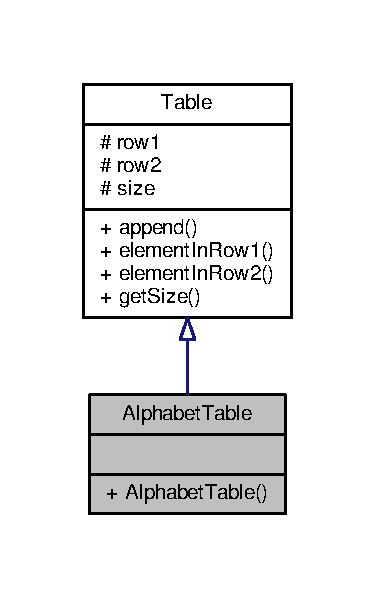
\includegraphics[width=180pt]{classAlphabetTable__inherit__graph}
\end{center}
\end{figure}


Collaboration diagram for Alphabet\+Table\+:
\nopagebreak
\begin{figure}[H]
\begin{center}
\leavevmode
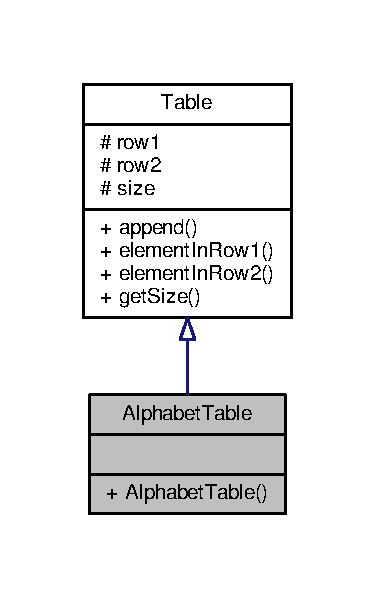
\includegraphics[width=180pt]{classAlphabetTable__coll__graph}
\end{center}
\end{figure}
\subsection*{Additional Inherited Members}


The documentation for this class was generated from the following files\+:\begin{DoxyCompactItemize}
\item 
/home/douglas/generator2/alphabettable.\+h\item 
/home/douglas/generator2/alphabettable.\+cpp\end{DoxyCompactItemize}

\hypertarget{classBodmasQuestion}{}\section{Bodmas\+Question Class Reference}
\label{classBodmasQuestion}\index{Bodmas\+Question@{Bodmas\+Question}}


Inheritance diagram for Bodmas\+Question\+:
\nopagebreak
\begin{figure}[H]
\begin{center}
\leavevmode
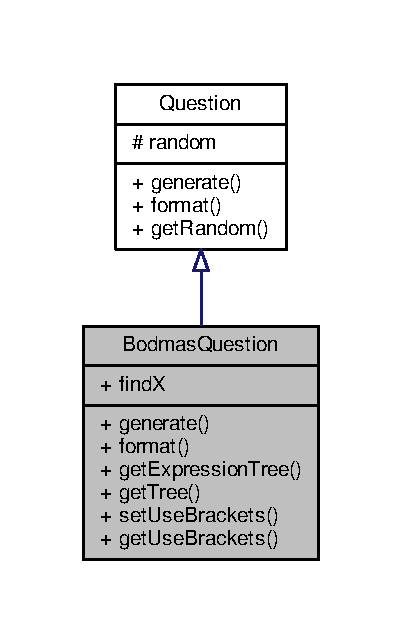
\includegraphics[width=193pt]{classBodmasQuestion__inherit__graph}
\end{center}
\end{figure}


Collaboration diagram for Bodmas\+Question\+:
\nopagebreak
\begin{figure}[H]
\begin{center}
\leavevmode
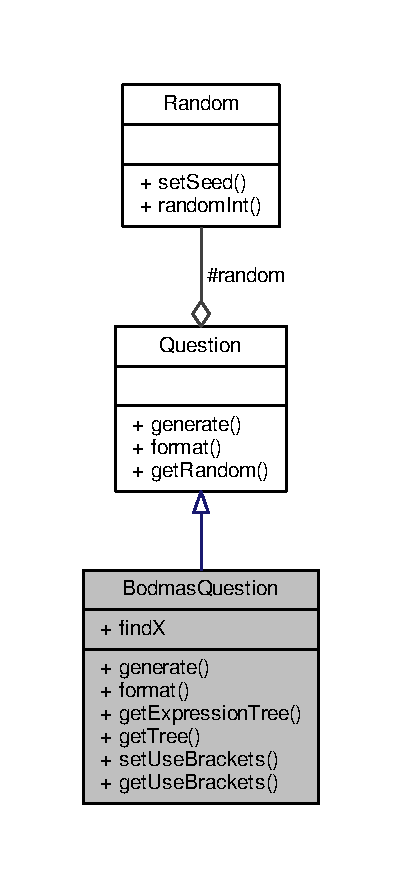
\includegraphics[width=193pt]{classBodmasQuestion__coll__graph}
\end{center}
\end{figure}
\subsection*{Public Member Functions}
\begin{DoxyCompactItemize}
\item 
virtual void {\bfseries generate} (std\+::vector$<$ std\+::string $>$ \&args)\hypertarget{classBodmasQuestion_a038609cfb6e17dea3ac335bf0fe6d860}{}\label{classBodmasQuestion_a038609cfb6e17dea3ac335bf0fe6d860}

\item 
virtual void {\bfseries format} (\hyperlink{classFormatter}{Formatter} $\ast$formatter)\hypertarget{classBodmasQuestion_a1e32206630a1df311ee5892005be441a}{}\label{classBodmasQuestion_a1e32206630a1df311ee5892005be441a}

\item 
\hyperlink{classExpressionTree}{Expression\+Tree} \& {\bfseries get\+Expression\+Tree} ()\hypertarget{classBodmasQuestion_a01cc51ae727f34521e39e8b723d3ea07}{}\label{classBodmasQuestion_a01cc51ae727f34521e39e8b723d3ea07}

\item 
\hyperlink{classTree}{Tree} $\ast$ {\bfseries get\+Tree} ()\hypertarget{classBodmasQuestion_ac274319dd340fa904b4a39f138265e8d}{}\label{classBodmasQuestion_ac274319dd340fa904b4a39f138265e8d}

\item 
void {\bfseries set\+Use\+Brackets} (bool b)\hypertarget{classBodmasQuestion_a13d0f843233d5423eb99727222e61a78}{}\label{classBodmasQuestion_a13d0f843233d5423eb99727222e61a78}

\item 
bool {\bfseries get\+Use\+Brackets} ()\hypertarget{classBodmasQuestion_affe33694bfa12a150e214f3e8eb3c1e7}{}\label{classBodmasQuestion_affe33694bfa12a150e214f3e8eb3c1e7}

\end{DoxyCompactItemize}
\subsection*{Public Attributes}
\begin{DoxyCompactItemize}
\item 
bool {\bfseries findX}\hypertarget{classBodmasQuestion_acc429143732f93192814cafa27987c2d}{}\label{classBodmasQuestion_acc429143732f93192814cafa27987c2d}

\end{DoxyCompactItemize}
\subsection*{Additional Inherited Members}


The documentation for this class was generated from the following files\+:\begin{DoxyCompactItemize}
\item 
/home/douglas/generator2/bodmasquestion.\+h\item 
/home/douglas/generator2/bodmasquestion.\+cpp\end{DoxyCompactItemize}

\hypertarget{classBodmasQuestionFormatter}{}\section{Bodmas\+Question\+Formatter Class Reference}
\label{classBodmasQuestionFormatter}\index{Bodmas\+Question\+Formatter@{Bodmas\+Question\+Formatter}}


Inheritance diagram for Bodmas\+Question\+Formatter\+:
\nopagebreak
\begin{figure}[H]
\begin{center}
\leavevmode
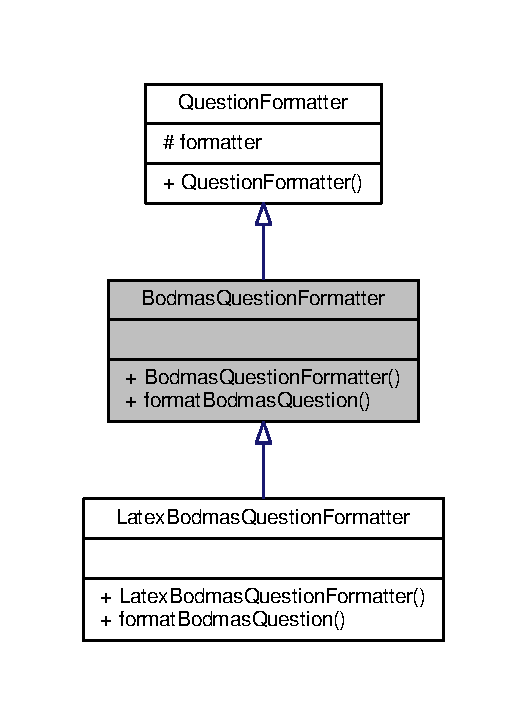
\includegraphics[width=253pt]{classBodmasQuestionFormatter__inherit__graph}
\end{center}
\end{figure}


Collaboration diagram for Bodmas\+Question\+Formatter\+:
\nopagebreak
\begin{figure}[H]
\begin{center}
\leavevmode
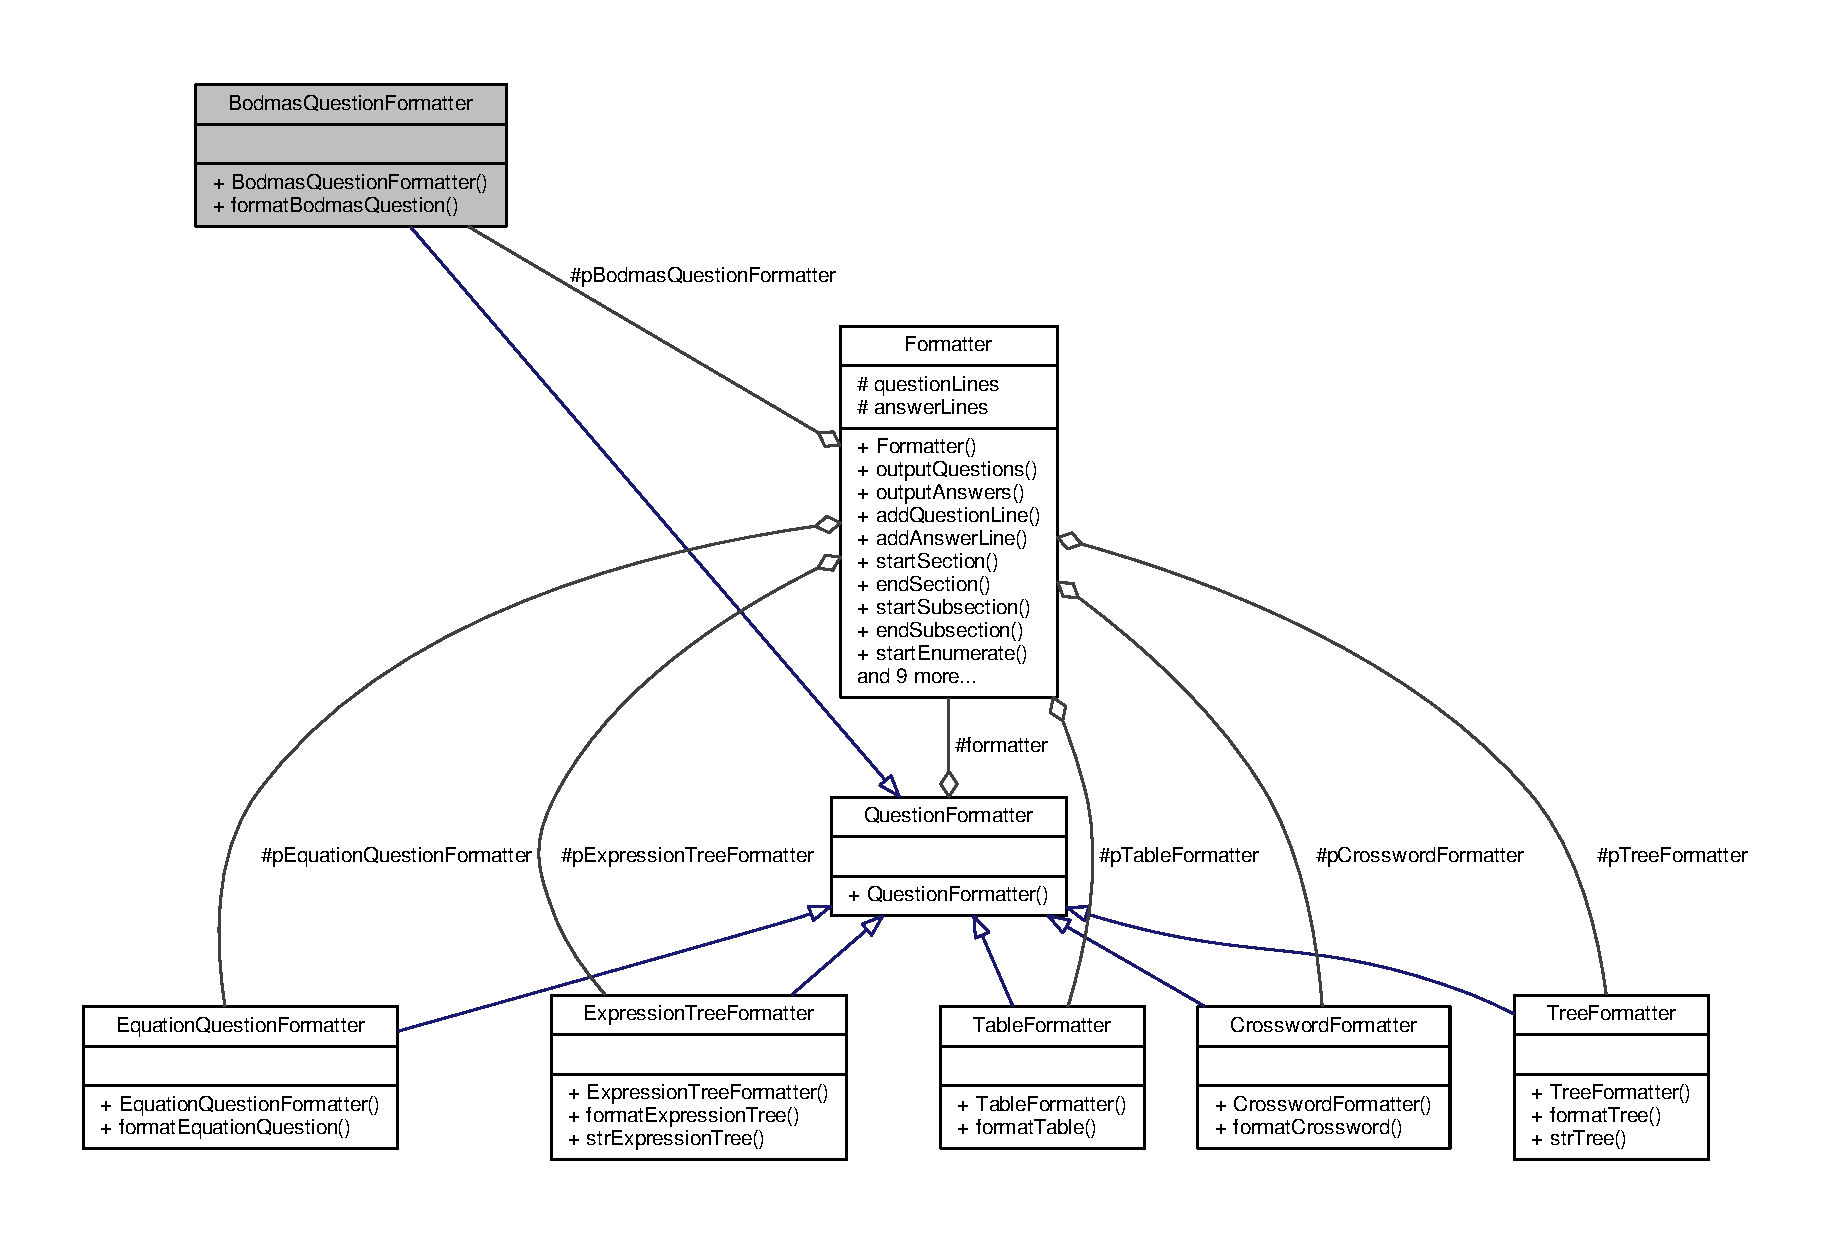
\includegraphics[width=350pt]{classBodmasQuestionFormatter__coll__graph}
\end{center}
\end{figure}
\subsection*{Public Member Functions}
\begin{DoxyCompactItemize}
\item 
{\bfseries Bodmas\+Question\+Formatter} (\hyperlink{classFormatter}{Formatter} $\ast$formatter)\hypertarget{classBodmasQuestionFormatter_a0c553ffeb33cdeb5a365840c5e8958e2}{}\label{classBodmasQuestionFormatter_a0c553ffeb33cdeb5a365840c5e8958e2}

\item 
virtual void {\bfseries format\+Bodmas\+Question} (\hyperlink{classBodmasQuestion}{Bodmas\+Question} $\ast$question)=0\hypertarget{classBodmasQuestionFormatter_afe7a1894127f1a2ff015caadfbfa3179}{}\label{classBodmasQuestionFormatter_afe7a1894127f1a2ff015caadfbfa3179}

\end{DoxyCompactItemize}
\subsection*{Additional Inherited Members}


The documentation for this class was generated from the following files\+:\begin{DoxyCompactItemize}
\item 
/home/douglas/generator2/bodmasquestionformatter.\+h\item 
/home/douglas/generator2/bodmasquestionformatter.\+cpp\end{DoxyCompactItemize}

\hypertarget{classBodmasQuestionVariant}{}\section{Bodmas\+Question\+Variant Class Reference}
\label{classBodmasQuestionVariant}\index{Bodmas\+Question\+Variant@{Bodmas\+Question\+Variant}}


Collaboration diagram for Bodmas\+Question\+Variant\+:
\nopagebreak
\begin{figure}[H]
\begin{center}
\leavevmode
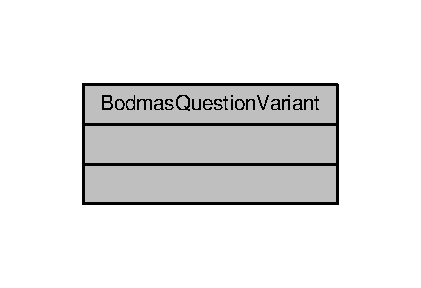
\includegraphics[width=202pt]{classBodmasQuestionVariant__coll__graph}
\end{center}
\end{figure}


The documentation for this class was generated from the following file\+:\begin{DoxyCompactItemize}
\item 
/home/douglas/generator2/bodmasquestionvariant.\+h\end{DoxyCompactItemize}

\hypertarget{classBodmasQuestionVariantTest}{}\section{Bodmas\+Question\+Variant\+Test Class Reference}
\label{classBodmasQuestionVariantTest}\index{Bodmas\+Question\+Variant\+Test@{Bodmas\+Question\+Variant\+Test}}


Collaboration diagram for Bodmas\+Question\+Variant\+Test\+:
\nopagebreak
\begin{figure}[H]
\begin{center}
\leavevmode
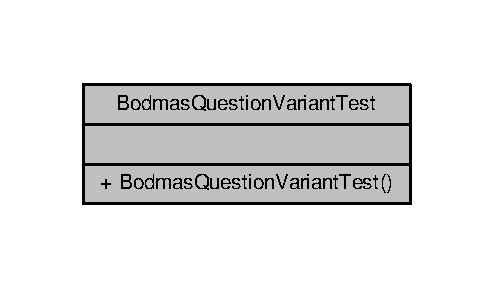
\includegraphics[width=237pt]{classBodmasQuestionVariantTest__coll__graph}
\end{center}
\end{figure}
\subsection*{Public Member Functions}
\begin{DoxyCompactItemize}
\item 
{\bfseries Bodmas\+Question\+Variant\+Test} (\hyperlink{classBodmasQuestion}{Bodmas\+Question} $\ast$question, std\+::vector$<$ std\+::string $>$ \&args)\hypertarget{classBodmasQuestionVariantTest_a17cf4ed12ca4012b4d11a54226191448}{}\label{classBodmasQuestionVariantTest_a17cf4ed12ca4012b4d11a54226191448}

\end{DoxyCompactItemize}


The documentation for this class was generated from the following files\+:\begin{DoxyCompactItemize}
\item 
/home/douglas/generator2/bodmasquestionvarianttest.\+h\item 
/home/douglas/generator2/bodmasquestionvarianttest.\+cpp\end{DoxyCompactItemize}

\hypertarget{classCharGrid}{}\section{Char\+Grid Class Reference}
\label{classCharGrid}\index{Char\+Grid@{Char\+Grid}}


Collaboration diagram for Char\+Grid\+:
\nopagebreak
\begin{figure}[H]
\begin{center}
\leavevmode
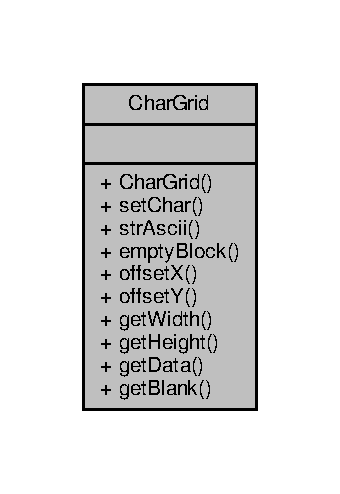
\includegraphics[width=163pt]{classCharGrid__coll__graph}
\end{center}
\end{figure}
\subsection*{Public Member Functions}
\begin{DoxyCompactItemize}
\item 
void {\bfseries set\+Char} (int x, int y, char c)\hypertarget{classCharGrid_a6617ec4da32eabd1f02fbadc4429eb59}{}\label{classCharGrid_a6617ec4da32eabd1f02fbadc4429eb59}

\item 
std\+::string {\bfseries str\+Ascii} ()\hypertarget{classCharGrid_abefadac3dbf2e1945e77bd41e715c8cc}{}\label{classCharGrid_abefadac3dbf2e1945e77bd41e715c8cc}

\item 
bool {\bfseries empty\+Block} (int x, int y)\hypertarget{classCharGrid_ac5a849bf687de48bc78b213992bea0f1}{}\label{classCharGrid_ac5a849bf687de48bc78b213992bea0f1}

\item 
int {\bfseries offsetX} (int x)\hypertarget{classCharGrid_a9dd1b0ebc5e58f3155b58fc143e6508b}{}\label{classCharGrid_a9dd1b0ebc5e58f3155b58fc143e6508b}

\item 
int {\bfseries offsetY} (int y)\hypertarget{classCharGrid_a187c68e52715cbbe753b20e5b458947c}{}\label{classCharGrid_a187c68e52715cbbe753b20e5b458947c}

\item 
int {\bfseries get\+Width} ()\hypertarget{classCharGrid_a50f4c607bb14624e0465a8f1fd7a6462}{}\label{classCharGrid_a50f4c607bb14624e0465a8f1fd7a6462}

\item 
int {\bfseries get\+Height} ()\hypertarget{classCharGrid_aeeb667243d37b38b8618eac646c07f69}{}\label{classCharGrid_aeeb667243d37b38b8618eac646c07f69}

\item 
std\+::deque$<$ std\+::string $>$ \& {\bfseries get\+Data} ()\hypertarget{classCharGrid_ad50d9c36ee0861dd994bf686f1afb537}{}\label{classCharGrid_ad50d9c36ee0861dd994bf686f1afb537}

\item 
char {\bfseries get\+Blank} ()\hypertarget{classCharGrid_a75a46545b1b48de3376b85929d5eb0c4}{}\label{classCharGrid_a75a46545b1b48de3376b85929d5eb0c4}

\end{DoxyCompactItemize}


The documentation for this class was generated from the following files\+:\begin{DoxyCompactItemize}
\item 
/home/douglas/generator2/chargrid.\+h\item 
/home/douglas/generator2/chargrid.\+cpp\end{DoxyCompactItemize}

\hypertarget{classCrossword}{}\section{Crossword Class Reference}
\label{classCrossword}\index{Crossword@{Crossword}}


Collaboration diagram for Crossword\+:
\nopagebreak
\begin{figure}[H]
\begin{center}
\leavevmode
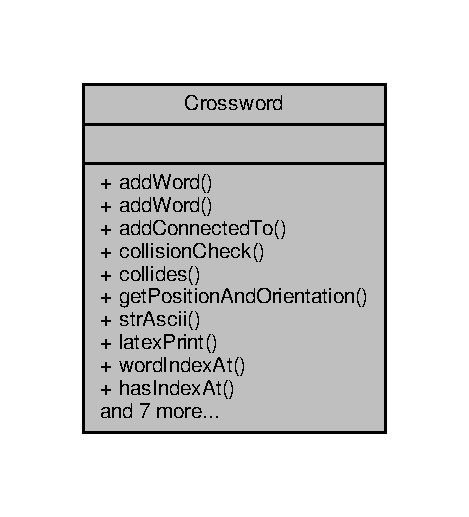
\includegraphics[width=225pt]{classCrossword__coll__graph}
\end{center}
\end{figure}
\subsection*{Public Member Functions}
\begin{DoxyCompactItemize}
\item 
bool {\bfseries add\+Word} (std\+::string word)\hypertarget{classCrossword_a8cd860c8c44d1b97e7667defb8a867ec}{}\label{classCrossword_a8cd860c8c44d1b97e7667defb8a867ec}

\item 
void {\bfseries add\+Word} (std\+::string word, int x, int y, bool across)\hypertarget{classCrossword_a264f80b2b16dc6ed81f8fcdb6668412a}{}\label{classCrossword_a264f80b2b16dc6ed81f8fcdb6668412a}

\item 
bool {\bfseries add\+Connected\+To} (std\+::string word, int wordI, std\+::string source\+Word, int source\+WordI)\hypertarget{classCrossword_aeb76f7a07b1dce37bcdb4f4c34d68096}{}\label{classCrossword_aeb76f7a07b1dce37bcdb4f4c34d68096}

\item 
bool {\bfseries collision\+Check} (std\+::string word, int x, int y, std\+::string source\+Word)\hypertarget{classCrossword_adffaf355b0ce0df1950aaf854df752db}{}\label{classCrossword_adffaf355b0ce0df1950aaf854df752db}

\item 
bool {\bfseries collides} (int abx, int aex, int aby, int aey, int bbx, int bex, int bby, int bey)\hypertarget{classCrossword_a3a7f13cd35e005add4e010c09ae47087}{}\label{classCrossword_a3a7f13cd35e005add4e010c09ae47087}

\item 
std\+::string {\bfseries get\+Position\+And\+Orientation} (const std\+::string \&word)\hypertarget{classCrossword_a9254e77677c936f3eb07baca7268f0f7}{}\label{classCrossword_a9254e77677c936f3eb07baca7268f0f7}

\item 
std\+::string {\bfseries str\+Ascii} ()\hypertarget{classCrossword_a9345fdb4c29eac51e4e2c3881d57f380}{}\label{classCrossword_a9345fdb4c29eac51e4e2c3881d57f380}

\item 
void {\bfseries latex\+Print} ()\hypertarget{classCrossword_a3f3b79bf83ea9bff5781214255a7576b}{}\label{classCrossword_a3f3b79bf83ea9bff5781214255a7576b}

\item 
int {\bfseries word\+Index\+At} (int x, int y)\hypertarget{classCrossword_a9072708ab5ecdae34bf8d6c7c5d3e65e}{}\label{classCrossword_a9072708ab5ecdae34bf8d6c7c5d3e65e}

\item 
bool {\bfseries has\+Index\+At} (int x, int y)\hypertarget{classCrossword_a08dacf55351f4cb07a7bd98bb17e40bc}{}\label{classCrossword_a08dacf55351f4cb07a7bd98bb17e40bc}

\item 
int {\bfseries index\+At} (int x, int y)\hypertarget{classCrossword_abb2f7fd9ec23c7543da4a031193dca9d}{}\label{classCrossword_abb2f7fd9ec23c7543da4a031193dca9d}

\item 
\hyperlink{classCharGrid}{Char\+Grid} \& {\bfseries get\+Grid} ()\hypertarget{classCrossword_a0e2eb976712cc19d99123ea00ca5a36b}{}\label{classCrossword_a0e2eb976712cc19d99123ea00ca5a36b}

\item 
void {\bfseries make\+Names} ()\hypertarget{classCrossword_adc255a20cadea9ddba13f8fc992da2a5}{}\label{classCrossword_adc255a20cadea9ddba13f8fc992da2a5}

\item 
std\+::string {\bfseries get\+Name\+Of} (std\+::string word)\hypertarget{classCrossword_afe1e74a939f5f0883a511f328e64b41d}{}\label{classCrossword_afe1e74a939f5f0883a511f328e64b41d}

\item 
std\+::vector$<$ std\+::string $>$ \& {\bfseries get\+Words\+In\+Order} ()\hypertarget{classCrossword_afff0c113751d2ffaf62358c91f400df9}{}\label{classCrossword_afff0c113751d2ffaf62358c91f400df9}

\item 
bool {\bfseries get\+Display\+Answers} ()\hypertarget{classCrossword_a90aac72a9259270a0d30d0acf760977c}{}\label{classCrossword_a90aac72a9259270a0d30d0acf760977c}

\item 
void {\bfseries set\+Display\+Answers} (bool b)\hypertarget{classCrossword_a4a5616c7b81bcc6902b79cc3634e047a}{}\label{classCrossword_a4a5616c7b81bcc6902b79cc3634e047a}

\end{DoxyCompactItemize}
\subsection*{Friends}
\begin{DoxyCompactItemize}
\item 
class {\bfseries Latex\+Crossword\+Printer}\hypertarget{classCrossword_ae525bd3dd94c2b1845a8d8fc7aae8ef7}{}\label{classCrossword_ae525bd3dd94c2b1845a8d8fc7aae8ef7}

\end{DoxyCompactItemize}


The documentation for this class was generated from the following files\+:\begin{DoxyCompactItemize}
\item 
/home/douglas/generator2/crossword.\+h\item 
/home/douglas/generator2/crossword.\+cpp\end{DoxyCompactItemize}

\hypertarget{classCrosswordFormatter}{}\section{Crossword\+Formatter Class Reference}
\label{classCrosswordFormatter}\index{Crossword\+Formatter@{Crossword\+Formatter}}


Inheritance diagram for Crossword\+Formatter\+:
\nopagebreak
\begin{figure}[H]
\begin{center}
\leavevmode
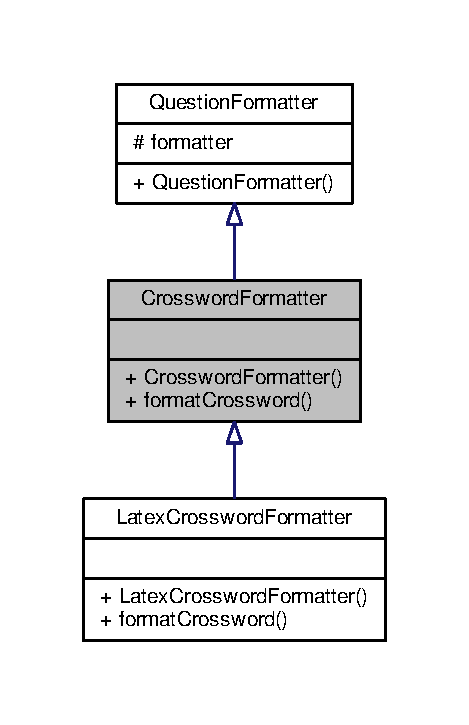
\includegraphics[width=225pt]{classCrosswordFormatter__inherit__graph}
\end{center}
\end{figure}


Collaboration diagram for Crossword\+Formatter\+:
\nopagebreak
\begin{figure}[H]
\begin{center}
\leavevmode
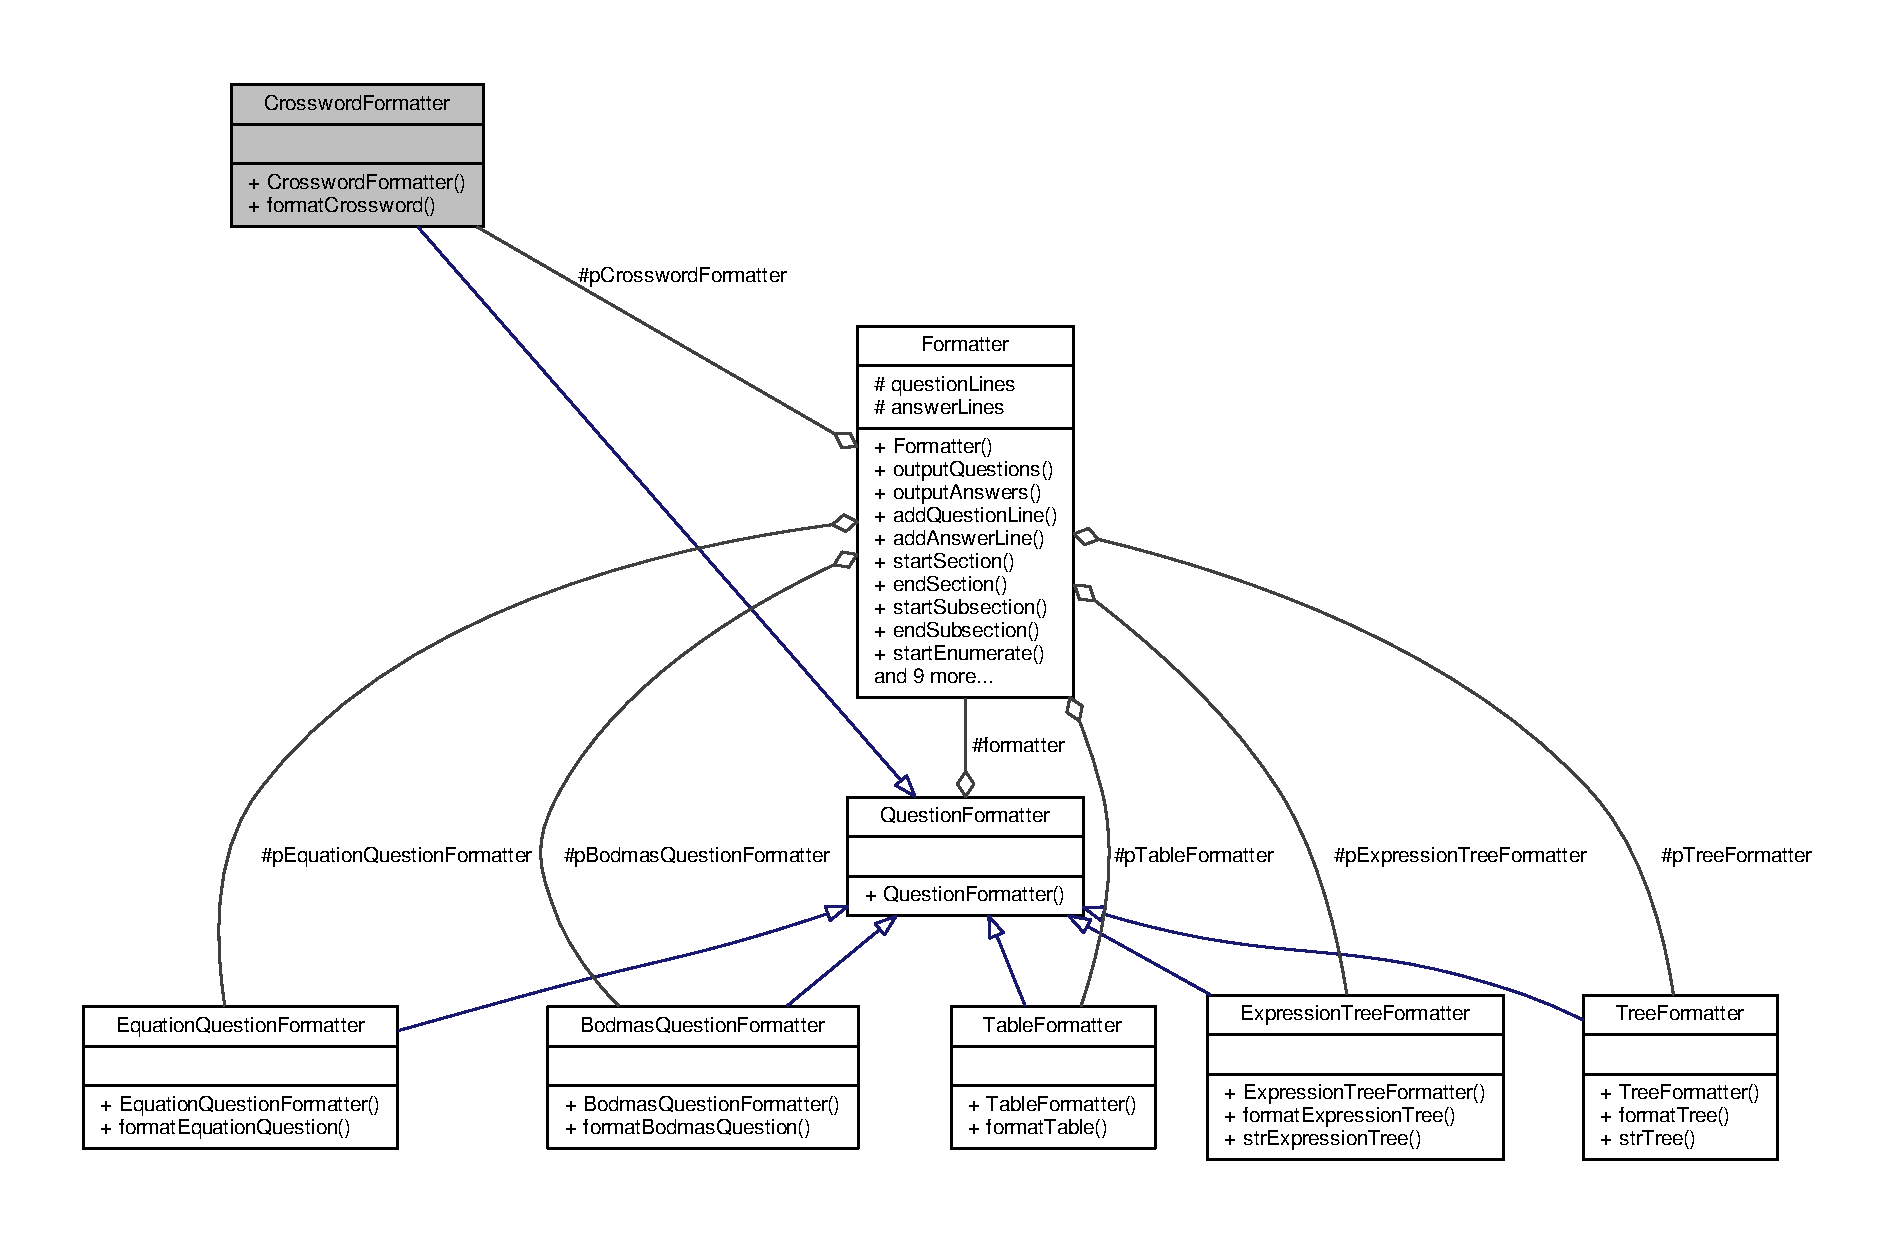
\includegraphics[width=350pt]{classCrosswordFormatter__coll__graph}
\end{center}
\end{figure}
\subsection*{Public Member Functions}
\begin{DoxyCompactItemize}
\item 
{\bfseries Crossword\+Formatter} (\hyperlink{classFormatter}{Formatter} $\ast$formatter)\hypertarget{classCrosswordFormatter_a2e35f71179c3e6cbd7aedd9d680bd8e4}{}\label{classCrosswordFormatter_a2e35f71179c3e6cbd7aedd9d680bd8e4}

\item 
virtual void {\bfseries format\+Crossword} (\hyperlink{classCrossword}{Crossword} $\ast$crossword)=0\hypertarget{classCrosswordFormatter_ad580e878ff44afc01cac77ff45e43d54}{}\label{classCrosswordFormatter_ad580e878ff44afc01cac77ff45e43d54}

\end{DoxyCompactItemize}
\subsection*{Additional Inherited Members}


The documentation for this class was generated from the following files\+:\begin{DoxyCompactItemize}
\item 
/home/douglas/generator2/crosswordformatter.\+h\item 
/home/douglas/generator2/crosswordformatter.\+cpp\end{DoxyCompactItemize}

\hypertarget{classCrosswordWorksheet}{}\section{Crossword\+Worksheet Class Reference}
\label{classCrosswordWorksheet}\index{Crossword\+Worksheet@{Crossword\+Worksheet}}


Inheritance diagram for Crossword\+Worksheet\+:
\nopagebreak
\begin{figure}[H]
\begin{center}
\leavevmode
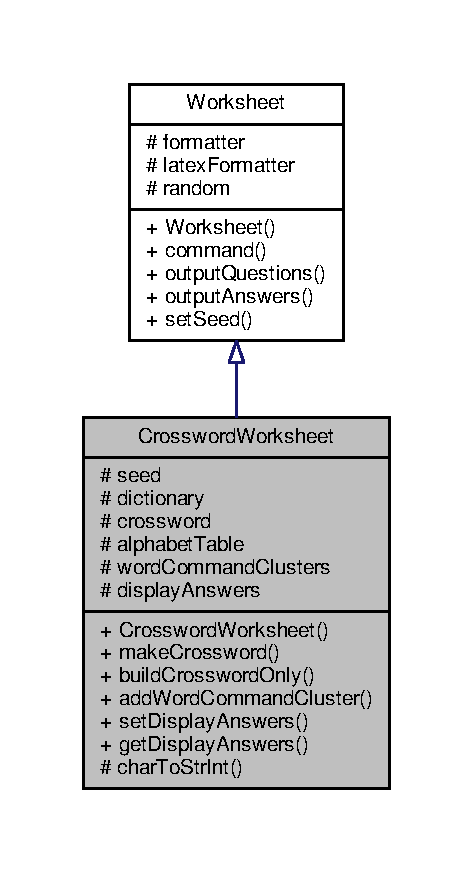
\includegraphics[width=227pt]{classCrosswordWorksheet__inherit__graph}
\end{center}
\end{figure}


Collaboration diagram for Crossword\+Worksheet\+:
\nopagebreak
\begin{figure}[H]
\begin{center}
\leavevmode
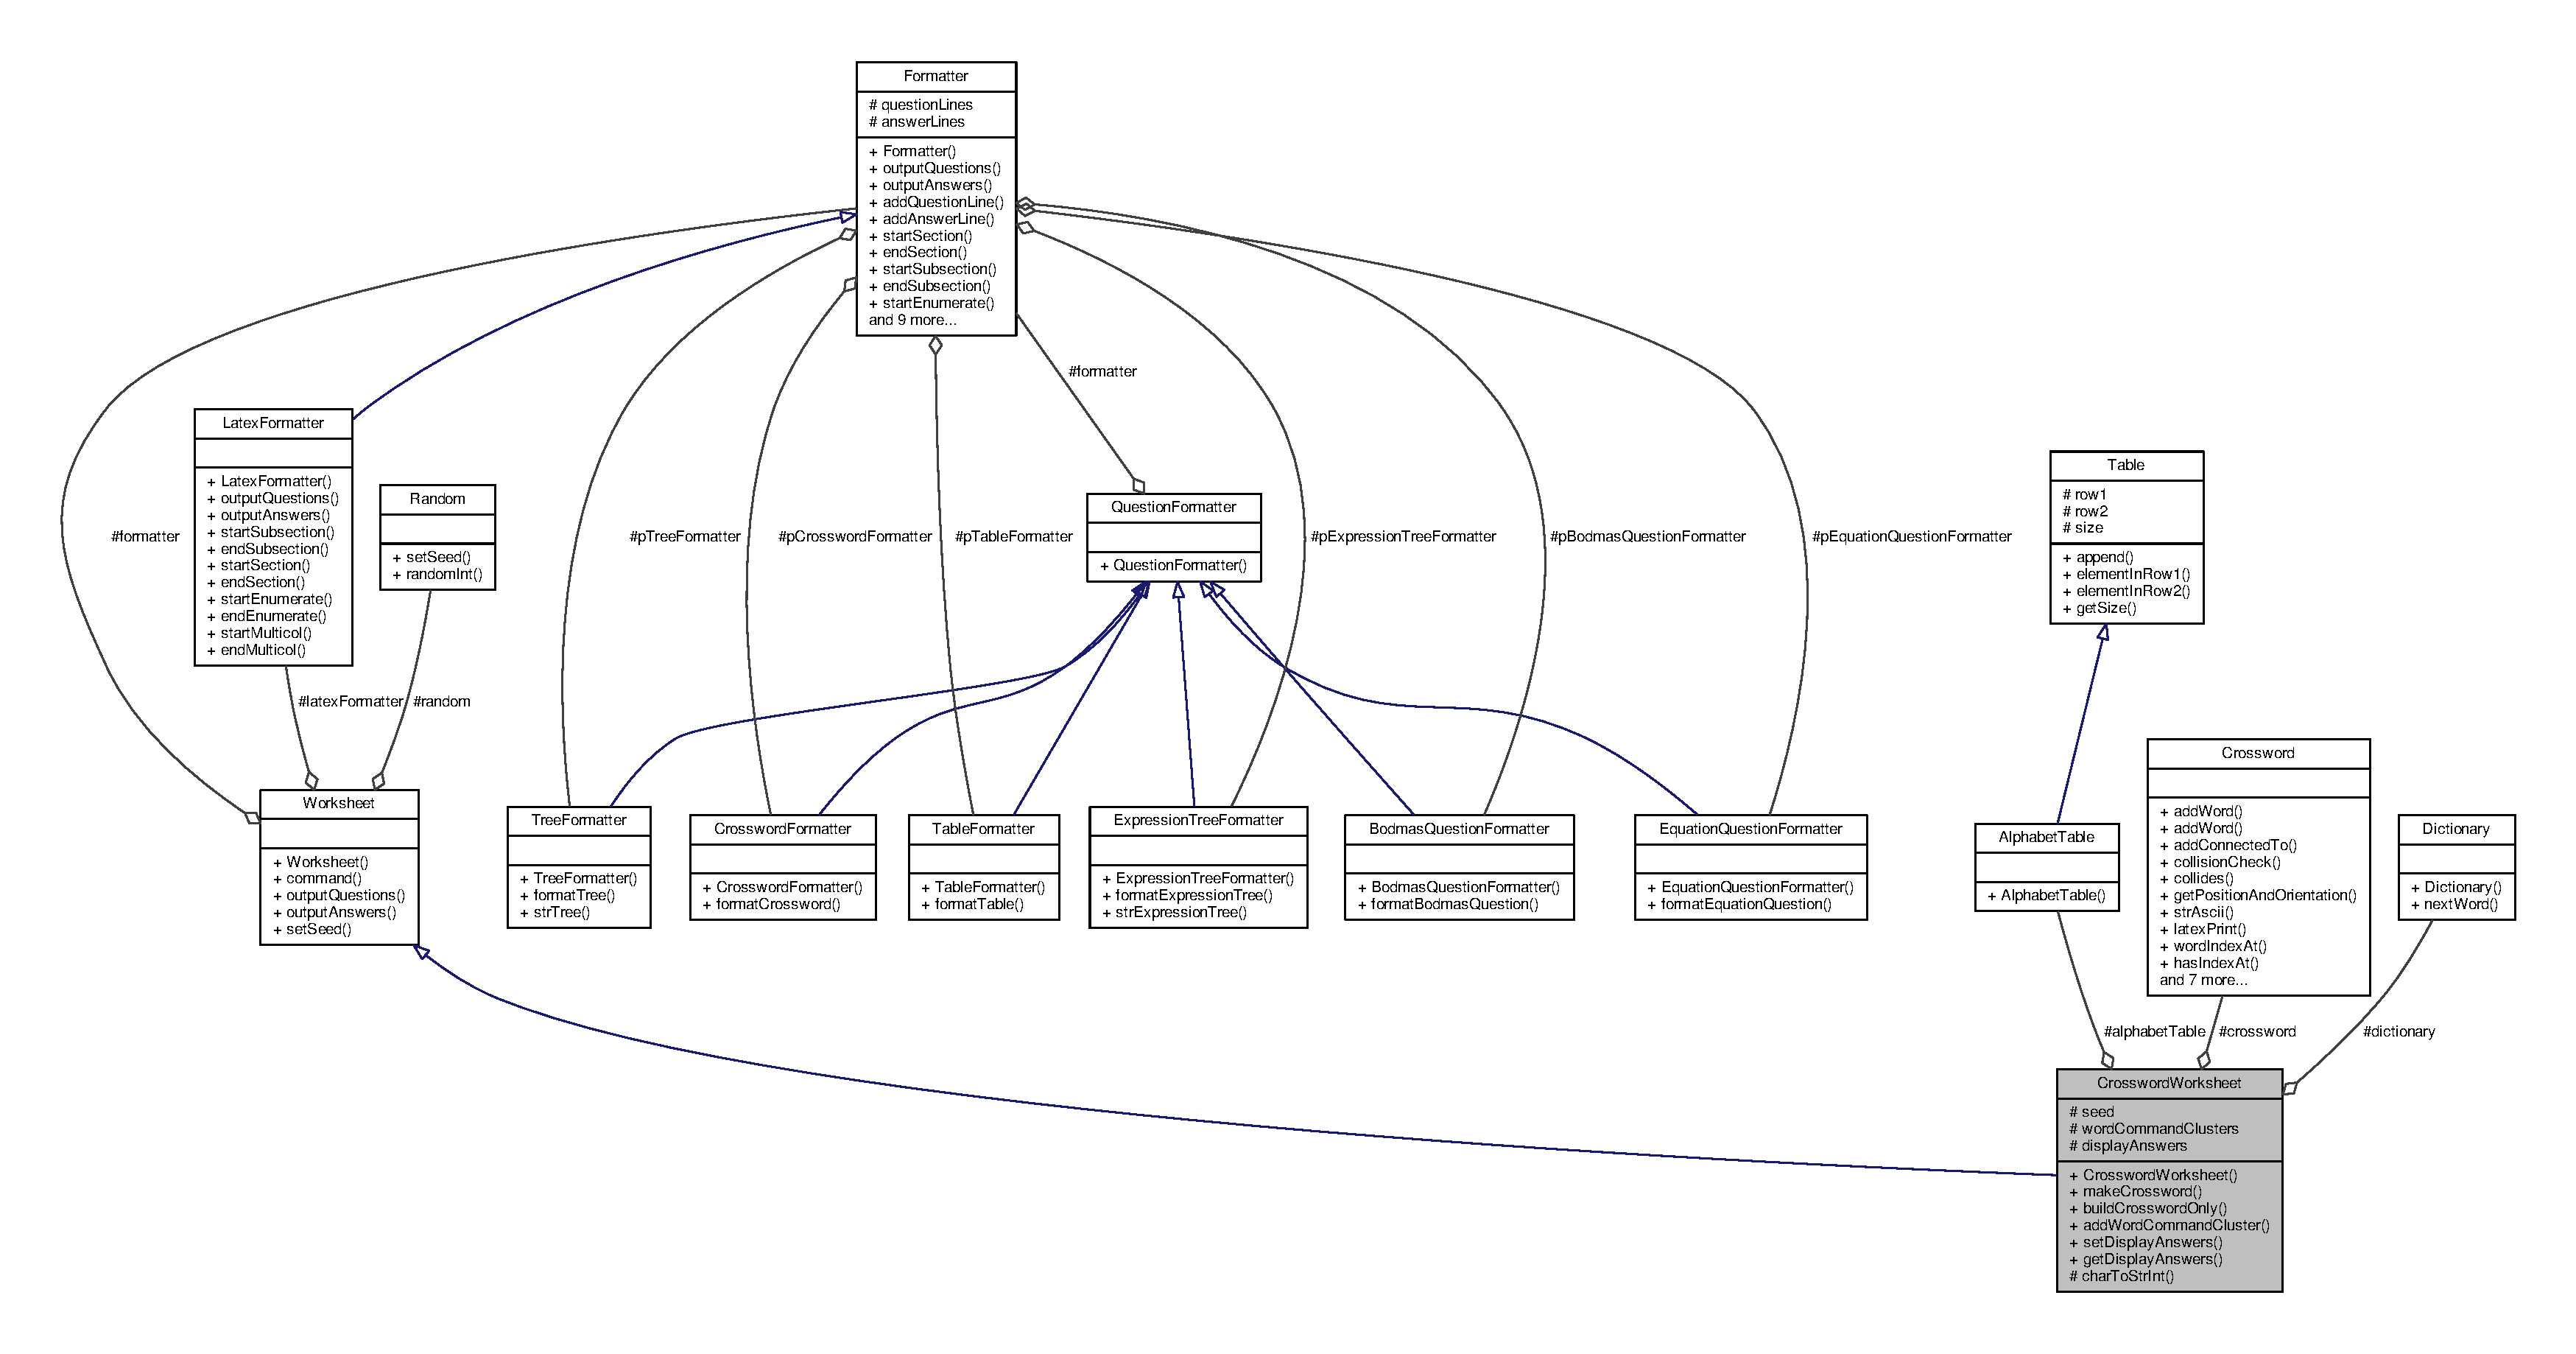
\includegraphics[width=350pt]{classCrosswordWorksheet__coll__graph}
\end{center}
\end{figure}
\subsection*{Public Member Functions}
\begin{DoxyCompactItemize}
\item 
void {\bfseries make\+Crossword} ()\hypertarget{classCrosswordWorksheet_ae71879c8a073e2582b1382f4d658cd60}{}\label{classCrosswordWorksheet_ae71879c8a073e2582b1382f4d658cd60}

\item 
void {\bfseries build\+Crossword\+Only} ()\hypertarget{classCrosswordWorksheet_a9be04af32644784bf72f3d055ceed5ac}{}\label{classCrosswordWorksheet_a9be04af32644784bf72f3d055ceed5ac}

\item 
void {\bfseries add\+Word\+Command\+Cluster} (std\+::string \&command)\hypertarget{classCrosswordWorksheet_affc342f3129caf2552beb6424f88ef9c}{}\label{classCrosswordWorksheet_affc342f3129caf2552beb6424f88ef9c}

\item 
void {\bfseries set\+Display\+Answers} (bool b)\hypertarget{classCrosswordWorksheet_a82e203edd8ddf4a3c5d820ae720ab614}{}\label{classCrosswordWorksheet_a82e203edd8ddf4a3c5d820ae720ab614}

\item 
bool {\bfseries get\+Display\+Answers} ()\hypertarget{classCrosswordWorksheet_ab6cf981c6dd95beeae33a37ea3871c51}{}\label{classCrosswordWorksheet_ab6cf981c6dd95beeae33a37ea3871c51}

\end{DoxyCompactItemize}
\subsection*{Protected Member Functions}
\begin{DoxyCompactItemize}
\item 
std\+::string {\bfseries char\+To\+Str\+Int} (char c)\hypertarget{classCrosswordWorksheet_aeb7b7acc71821fb7e2fd2edc259dbf95}{}\label{classCrosswordWorksheet_aeb7b7acc71821fb7e2fd2edc259dbf95}

\end{DoxyCompactItemize}
\subsection*{Protected Attributes}
\begin{DoxyCompactItemize}
\item 
int {\bfseries seed}\hypertarget{classCrosswordWorksheet_ac209b0c433b65f48bda15b9b214b068b}{}\label{classCrosswordWorksheet_ac209b0c433b65f48bda15b9b214b068b}

\item 
\hyperlink{classDictionary}{Dictionary} {\bfseries dictionary}\hypertarget{classCrosswordWorksheet_a27a603575ccdad7641e889fc2d86a0ae}{}\label{classCrosswordWorksheet_a27a603575ccdad7641e889fc2d86a0ae}

\item 
\hyperlink{classCrossword}{Crossword} {\bfseries crossword}\hypertarget{classCrosswordWorksheet_aca55a414575d6ebbdcbfb1f4b92761c1}{}\label{classCrosswordWorksheet_aca55a414575d6ebbdcbfb1f4b92761c1}

\item 
\hyperlink{classAlphabetTable}{Alphabet\+Table} {\bfseries alphabet\+Table}\hypertarget{classCrosswordWorksheet_afc3406772bf2414fb0d1639f324ed250}{}\label{classCrosswordWorksheet_afc3406772bf2414fb0d1639f324ed250}

\item 
std\+::vector$<$ std\+::string $>$ {\bfseries word\+Command\+Clusters}\hypertarget{classCrosswordWorksheet_a998510a83bc44f411880708806b3db57}{}\label{classCrosswordWorksheet_a998510a83bc44f411880708806b3db57}

\item 
bool {\bfseries display\+Answers}\hypertarget{classCrosswordWorksheet_afc79a534c0add705a7e12d5698cc90ce}{}\label{classCrosswordWorksheet_afc79a534c0add705a7e12d5698cc90ce}

\end{DoxyCompactItemize}


The documentation for this class was generated from the following files\+:\begin{DoxyCompactItemize}
\item 
/home/douglas/generator2/crosswordworksheet.\+h\item 
/home/douglas/generator2/crosswordworksheet.\+cpp\end{DoxyCompactItemize}

\hypertarget{classDictionary}{}\section{Dictionary Class Reference}
\label{classDictionary}\index{Dictionary@{Dictionary}}


Collaboration diagram for Dictionary\+:
\nopagebreak
\begin{figure}[H]
\begin{center}
\leavevmode
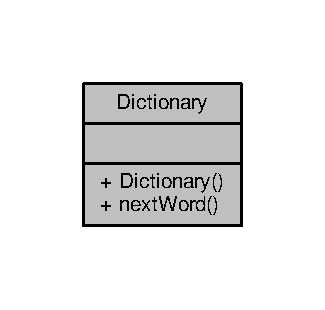
\includegraphics[width=156pt]{classDictionary__coll__graph}
\end{center}
\end{figure}
\subsection*{Public Member Functions}
\begin{DoxyCompactItemize}
\item 
std\+::string \& {\bfseries next\+Word} (\hyperlink{classRandom}{Random} $\ast$random)\hypertarget{classDictionary_aa8accefaff6f64e221ead60982f6dd07}{}\label{classDictionary_aa8accefaff6f64e221ead60982f6dd07}

\end{DoxyCompactItemize}


The documentation for this class was generated from the following files\+:\begin{DoxyCompactItemize}
\item 
/home/douglas/generator2/dictionary.\+h\item 
/home/douglas/generator2/dictionary.\+cpp\end{DoxyCompactItemize}

\hypertarget{classEquationQuestion}{}\section{Equation\+Question Class Reference}
\label{classEquationQuestion}\index{Equation\+Question@{Equation\+Question}}


Inheritance diagram for Equation\+Question\+:
\nopagebreak
\begin{figure}[H]
\begin{center}
\leavevmode
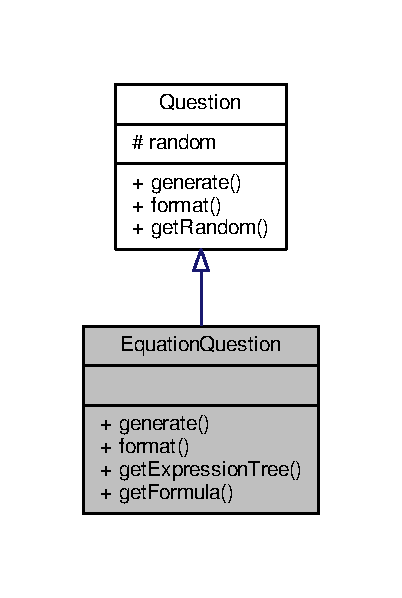
\includegraphics[width=193pt]{classEquationQuestion__inherit__graph}
\end{center}
\end{figure}


Collaboration diagram for Equation\+Question\+:
\nopagebreak
\begin{figure}[H]
\begin{center}
\leavevmode
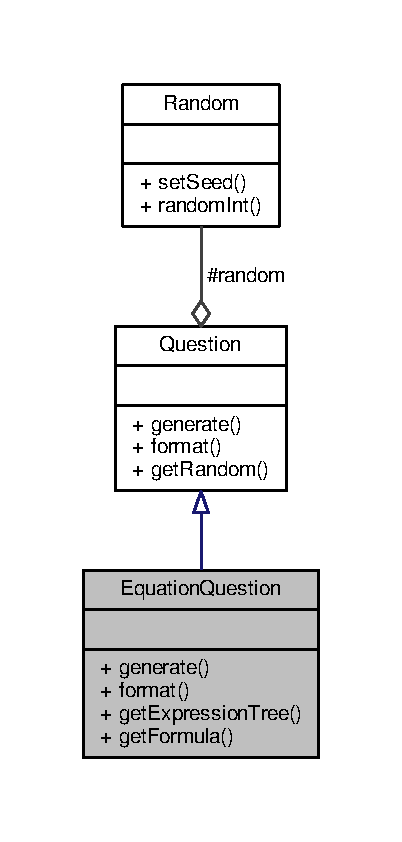
\includegraphics[width=193pt]{classEquationQuestion__coll__graph}
\end{center}
\end{figure}
\subsection*{Public Member Functions}
\begin{DoxyCompactItemize}
\item 
virtual void {\bfseries generate} (std\+::vector$<$ std\+::string $>$ \&args)\hypertarget{classEquationQuestion_a5779f4c91db396c3db9cdf7e2b26ccfa}{}\label{classEquationQuestion_a5779f4c91db396c3db9cdf7e2b26ccfa}

\item 
virtual void {\bfseries format} (\hyperlink{classFormatter}{Formatter} $\ast$formatter)\hypertarget{classEquationQuestion_a1a6c52b71d040d7ae01166a13719e6c8}{}\label{classEquationQuestion_a1a6c52b71d040d7ae01166a13719e6c8}

\item 
\hyperlink{classExpressionTree}{Expression\+Tree} \& {\bfseries get\+Expression\+Tree} ()\hypertarget{classEquationQuestion_a2cf99e4b721119b32fca972312baebd8}{}\label{classEquationQuestion_a2cf99e4b721119b32fca972312baebd8}

\item 
\hyperlink{classFormula}{Formula} \& {\bfseries get\+Formula} ()\hypertarget{classEquationQuestion_a23040188b5055d7ed1acdde4334f0fce}{}\label{classEquationQuestion_a23040188b5055d7ed1acdde4334f0fce}

\end{DoxyCompactItemize}
\subsection*{Additional Inherited Members}


The documentation for this class was generated from the following files\+:\begin{DoxyCompactItemize}
\item 
/home/douglas/generator2/equationquestion.\+h\item 
/home/douglas/generator2/equationquestion.\+cpp\end{DoxyCompactItemize}

\hypertarget{classEquationQuestionFormatter}{}\section{Equation\+Question\+Formatter Class Reference}
\label{classEquationQuestionFormatter}\index{Equation\+Question\+Formatter@{Equation\+Question\+Formatter}}


Inheritance diagram for Equation\+Question\+Formatter\+:
\nopagebreak
\begin{figure}[H]
\begin{center}
\leavevmode
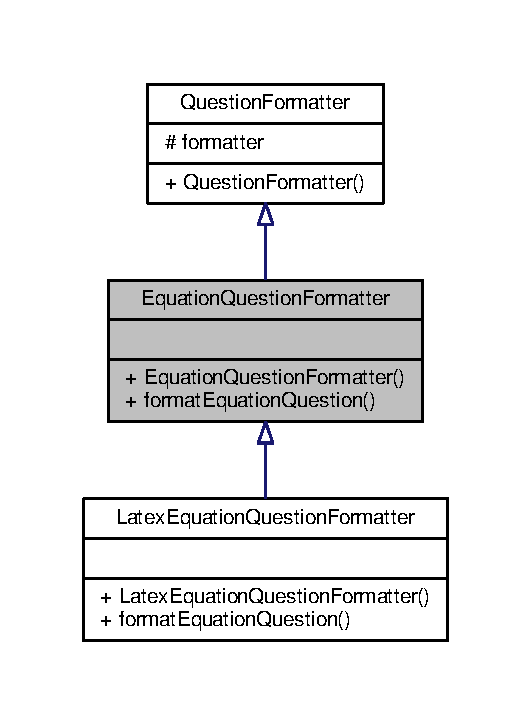
\includegraphics[width=255pt]{classEquationQuestionFormatter__inherit__graph}
\end{center}
\end{figure}


Collaboration diagram for Equation\+Question\+Formatter\+:
\nopagebreak
\begin{figure}[H]
\begin{center}
\leavevmode
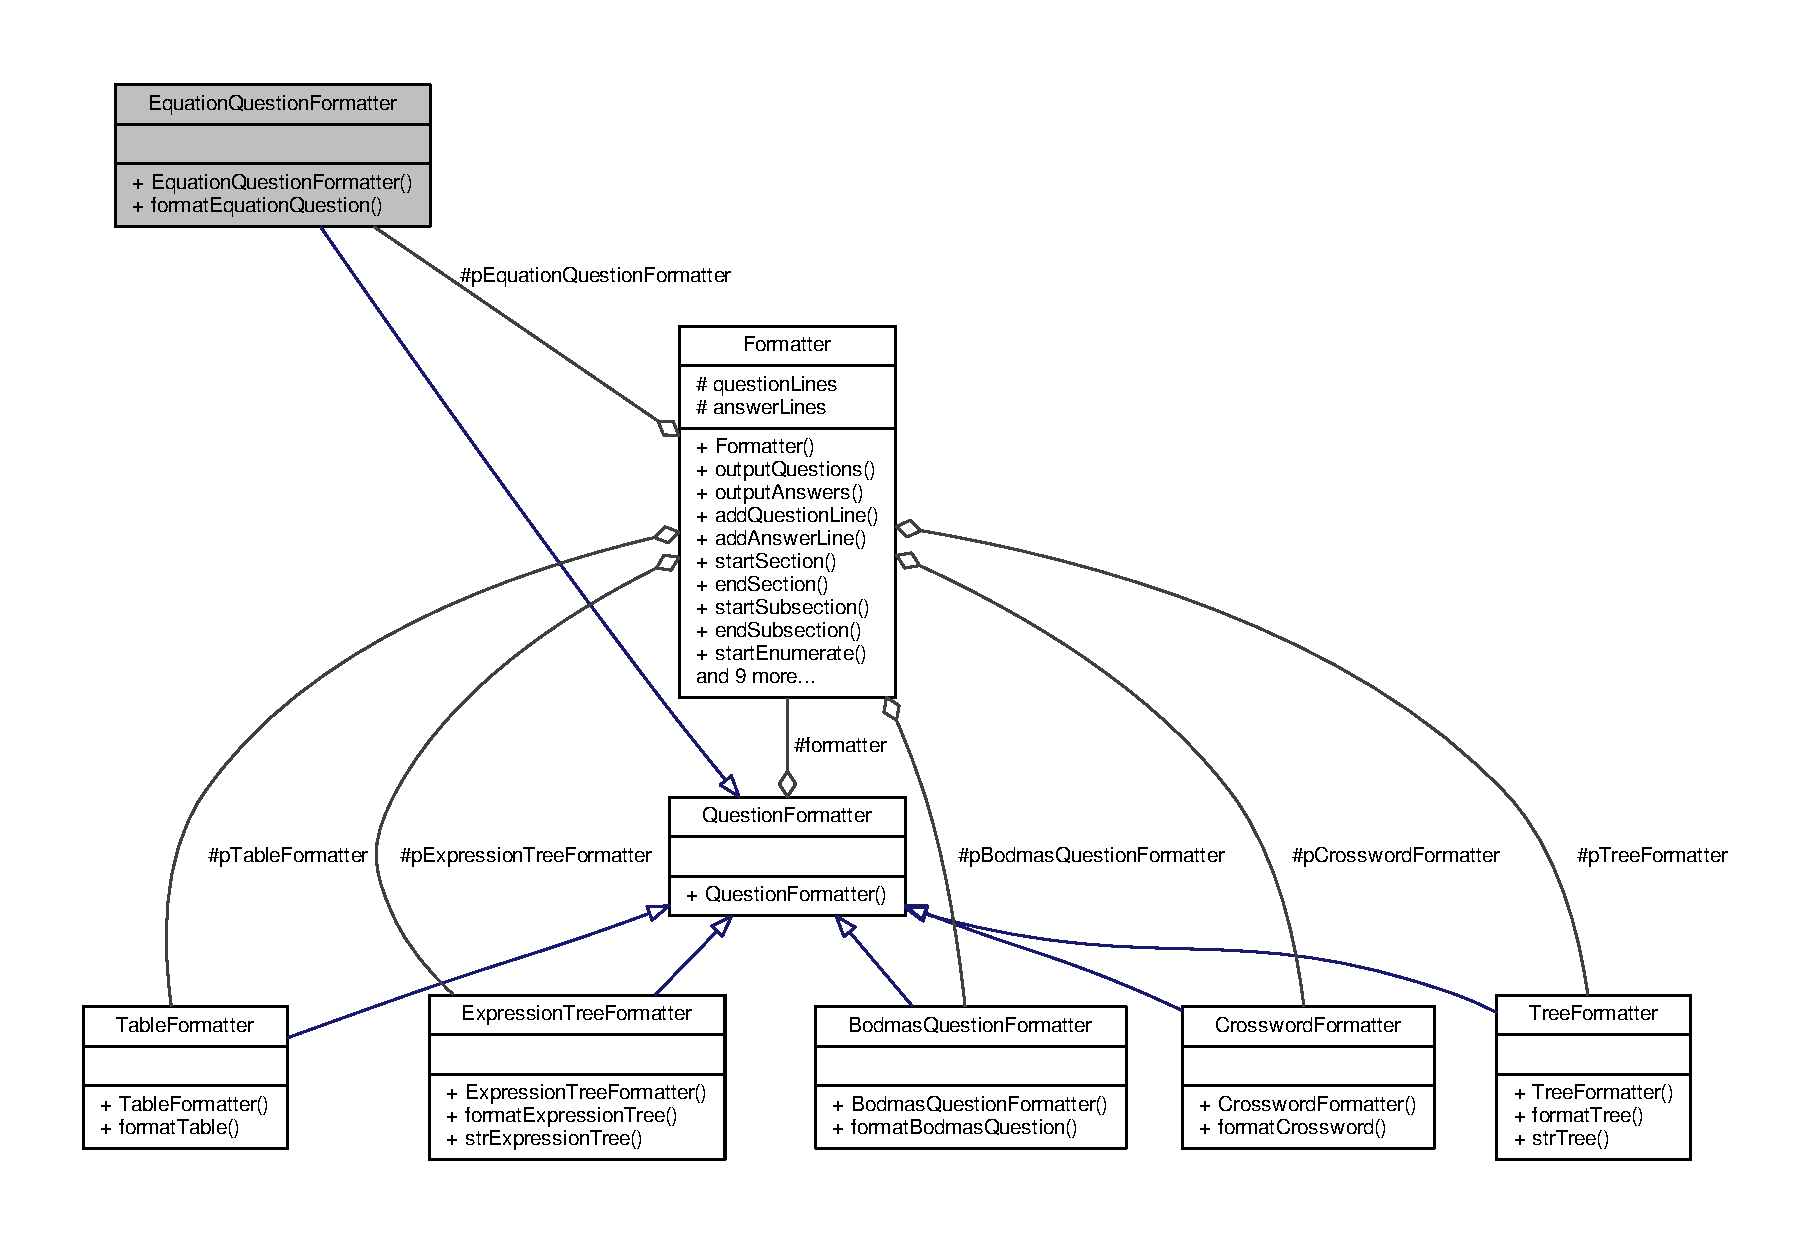
\includegraphics[width=350pt]{classEquationQuestionFormatter__coll__graph}
\end{center}
\end{figure}
\subsection*{Public Member Functions}
\begin{DoxyCompactItemize}
\item 
{\bfseries Equation\+Question\+Formatter} (\hyperlink{classFormatter}{Formatter} $\ast$formatter)\hypertarget{classEquationQuestionFormatter_a4dba4c709554a25c0cdb5831969ce1e7}{}\label{classEquationQuestionFormatter_a4dba4c709554a25c0cdb5831969ce1e7}

\item 
virtual void {\bfseries format\+Equation\+Question} (\hyperlink{classEquationQuestion}{Equation\+Question} $\ast$question)=0\hypertarget{classEquationQuestionFormatter_aca8548fb0d28dc9e41756976e392604e}{}\label{classEquationQuestionFormatter_aca8548fb0d28dc9e41756976e392604e}

\end{DoxyCompactItemize}
\subsection*{Additional Inherited Members}


The documentation for this class was generated from the following files\+:\begin{DoxyCompactItemize}
\item 
/home/douglas/generator2/equationquestionformatter.\+h\item 
/home/douglas/generator2/equationquestionformatter.\+cpp\end{DoxyCompactItemize}

\hypertarget{classEquationQuestionVariant}{}\section{Equation\+Question\+Variant Class Reference}
\label{classEquationQuestionVariant}\index{Equation\+Question\+Variant@{Equation\+Question\+Variant}}


Inheritance diagram for Equation\+Question\+Variant\+:
\nopagebreak
\begin{figure}[H]
\begin{center}
\leavevmode
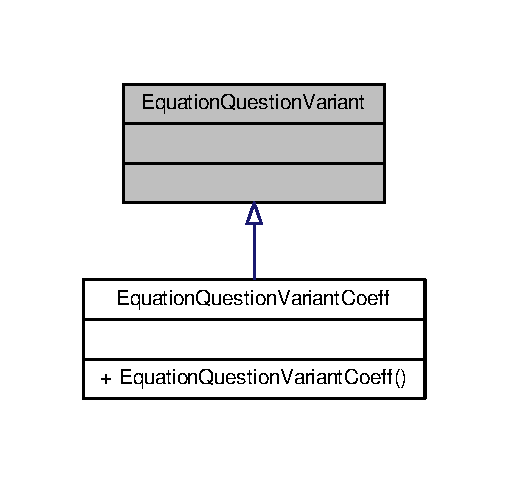
\includegraphics[width=244pt]{classEquationQuestionVariant__inherit__graph}
\end{center}
\end{figure}


Collaboration diagram for Equation\+Question\+Variant\+:
\nopagebreak
\begin{figure}[H]
\begin{center}
\leavevmode
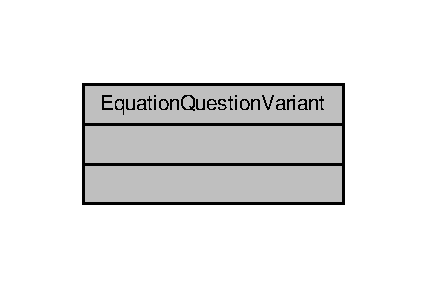
\includegraphics[width=205pt]{classEquationQuestionVariant__coll__graph}
\end{center}
\end{figure}


The documentation for this class was generated from the following file\+:\begin{DoxyCompactItemize}
\item 
/home/douglas/generator2/equationquestionvariant.\+h\end{DoxyCompactItemize}

\hypertarget{classEquationQuestionVariantCoeff}{}\section{Equation\+Question\+Variant\+Coeff Class Reference}
\label{classEquationQuestionVariantCoeff}\index{Equation\+Question\+Variant\+Coeff@{Equation\+Question\+Variant\+Coeff}}


Inheritance diagram for Equation\+Question\+Variant\+Coeff\+:
\nopagebreak
\begin{figure}[H]
\begin{center}
\leavevmode
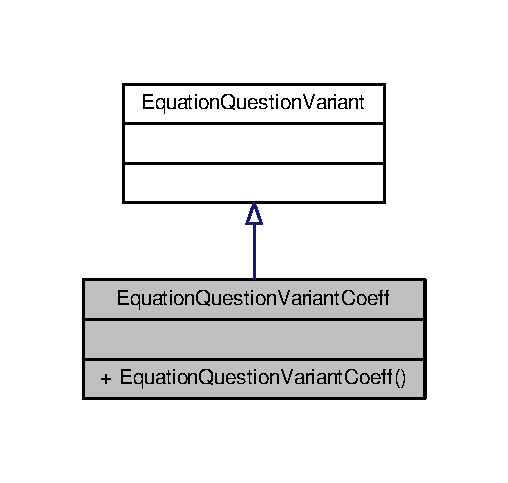
\includegraphics[width=244pt]{classEquationQuestionVariantCoeff__inherit__graph}
\end{center}
\end{figure}


Collaboration diagram for Equation\+Question\+Variant\+Coeff\+:
\nopagebreak
\begin{figure}[H]
\begin{center}
\leavevmode
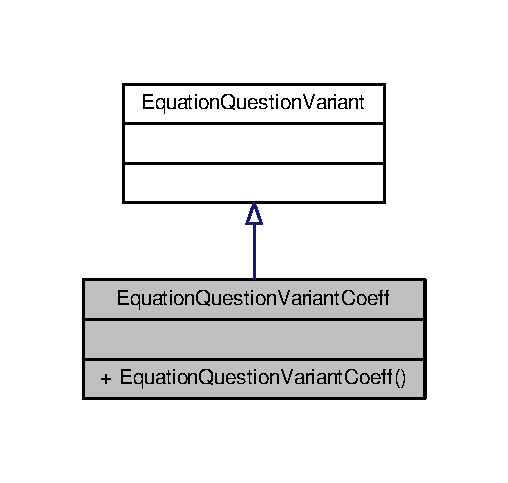
\includegraphics[width=244pt]{classEquationQuestionVariantCoeff__coll__graph}
\end{center}
\end{figure}
\subsection*{Public Member Functions}
\begin{DoxyCompactItemize}
\item 
{\bfseries Equation\+Question\+Variant\+Coeff} (std\+::vector$<$ std\+::string $>$ \&args, \hyperlink{classEquationQuestion}{Equation\+Question} $\ast$question)\hypertarget{classEquationQuestionVariantCoeff_ad1e019414db35d6f1be8a2c125a91294}{}\label{classEquationQuestionVariantCoeff_ad1e019414db35d6f1be8a2c125a91294}

\end{DoxyCompactItemize}


The documentation for this class was generated from the following files\+:\begin{DoxyCompactItemize}
\item 
/home/douglas/generator2/equationquestionvariantcoeff.\+h\item 
/home/douglas/generator2/equationquestionvariantcoeff.\+cpp\end{DoxyCompactItemize}

\hypertarget{classExpressionNode}{}\section{Expression\+Node Class Reference}
\label{classExpressionNode}\index{Expression\+Node@{Expression\+Node}}


Collaboration diagram for Expression\+Node\+:
\nopagebreak
\begin{figure}[H]
\begin{center}
\leavevmode
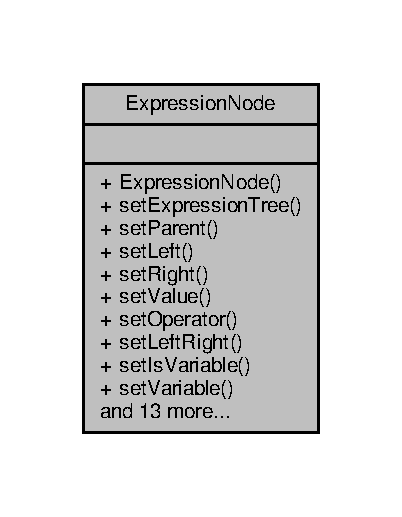
\includegraphics[width=193pt]{classExpressionNode__coll__graph}
\end{center}
\end{figure}
\subsection*{Public Types}
\begin{DoxyCompactItemize}
\item 
enum {\bfseries Operator} \{ \\*
{\bfseries N\+O\+NE} = 0, 
{\bfseries P\+L\+US}, 
{\bfseries M\+I\+N\+US}, 
{\bfseries T\+I\+M\+ES}, 
\\*
{\bfseries D\+I\+V\+I\+DE}, 
{\bfseries F\+R\+AC}, 
{\bfseries E\+XP}, 
{\bfseries R\+O\+OT}
 \}\hypertarget{classExpressionNode_a7735465f9aac516880869e4a630d2569}{}\label{classExpressionNode_a7735465f9aac516880869e4a630d2569}

\end{DoxyCompactItemize}
\subsection*{Public Member Functions}
\begin{DoxyCompactItemize}
\item 
void {\bfseries set\+Expression\+Tree} (\hyperlink{classExpressionTree}{Expression\+Tree} $\ast$expression\+Tree)\hypertarget{classExpressionNode_a97010b6f697941a0522f1f13a55e1537}{}\label{classExpressionNode_a97010b6f697941a0522f1f13a55e1537}

\item 
void {\bfseries set\+Parent} (\hyperlink{classExpressionNode}{Expression\+Node} $\ast$parent)\hypertarget{classExpressionNode_aeed821d5466822cf6c84a16edd88428b}{}\label{classExpressionNode_aeed821d5466822cf6c84a16edd88428b}

\item 
void {\bfseries set\+Left} (\hyperlink{classExpressionNode}{Expression\+Node} $\ast$left)\hypertarget{classExpressionNode_a4a1082d2ef3d4eb90c88d45ff7b3c92e}{}\label{classExpressionNode_a4a1082d2ef3d4eb90c88d45ff7b3c92e}

\item 
void {\bfseries set\+Right} (\hyperlink{classExpressionNode}{Expression\+Node} $\ast$right)\hypertarget{classExpressionNode_ad123db23336006f9d37458dfcd240158}{}\label{classExpressionNode_ad123db23336006f9d37458dfcd240158}

\item 
void {\bfseries set\+Value} (int value)\hypertarget{classExpressionNode_a84c28fcc2296c5d6cfa8a71595cee32d}{}\label{classExpressionNode_a84c28fcc2296c5d6cfa8a71595cee32d}

\item 
void {\bfseries set\+Operator} (int op)\hypertarget{classExpressionNode_ac4c9f6574b462191267c2a43f64503ec}{}\label{classExpressionNode_ac4c9f6574b462191267c2a43f64503ec}

\item 
void {\bfseries set\+Left\+Right} (\hyperlink{classExpressionNode}{Expression\+Node} $\ast$left, \hyperlink{classExpressionNode}{Expression\+Node} $\ast$right)\hypertarget{classExpressionNode_a27a7dbaa192ed918f2485c9f67389f7a}{}\label{classExpressionNode_a27a7dbaa192ed918f2485c9f67389f7a}

\item 
void {\bfseries set\+Is\+Variable} (bool b)\hypertarget{classExpressionNode_af142d717316c6b0d5cdba9cef7240cca}{}\label{classExpressionNode_af142d717316c6b0d5cdba9cef7240cca}

\item 
void {\bfseries set\+Variable} (char variable)\hypertarget{classExpressionNode_a1b7d69d73e5c84484fa8d4221530620e}{}\label{classExpressionNode_a1b7d69d73e5c84484fa8d4221530620e}

\item 
\hyperlink{classExpressionTree}{Expression\+Tree} $\ast$ {\bfseries get\+Expression\+Tree} ()\hypertarget{classExpressionNode_a65d4aef39850ffaeadad4a5385c8e986}{}\label{classExpressionNode_a65d4aef39850ffaeadad4a5385c8e986}

\item 
\hyperlink{classExpressionNode}{Expression\+Node} $\ast$ {\bfseries get\+Parent} ()\hypertarget{classExpressionNode_af273e8a6b5f8336931d32984d71e62ee}{}\label{classExpressionNode_af273e8a6b5f8336931d32984d71e62ee}

\item 
\hyperlink{classExpressionNode}{Expression\+Node} $\ast$ {\bfseries get\+Left} ()\hypertarget{classExpressionNode_a9818bdb068e0849c4691a5db7c4bbcbf}{}\label{classExpressionNode_a9818bdb068e0849c4691a5db7c4bbcbf}

\item 
\hyperlink{classExpressionNode}{Expression\+Node} $\ast$ {\bfseries get\+Right} ()\hypertarget{classExpressionNode_ac3e6362584c8057ebbbc14326f54b50c}{}\label{classExpressionNode_ac3e6362584c8057ebbbc14326f54b50c}

\item 
int {\bfseries get\+Value} ()\hypertarget{classExpressionNode_a8b4cd85947782998da3a67649afd1b97}{}\label{classExpressionNode_a8b4cd85947782998da3a67649afd1b97}

\item 
int {\bfseries get\+Operator} ()\hypertarget{classExpressionNode_a4b289464ef13fb5a06fe250aef5081a4}{}\label{classExpressionNode_a4b289464ef13fb5a06fe250aef5081a4}

\item 
bool {\bfseries get\+Is\+Variable} ()\hypertarget{classExpressionNode_a078b875f649fe63ffdd8642fbb549843}{}\label{classExpressionNode_a078b875f649fe63ffdd8642fbb549843}

\item 
char {\bfseries get\+Variable} ()\hypertarget{classExpressionNode_a5e3e02cb0e049885fa4a71ba976f96da}{}\label{classExpressionNode_a5e3e02cb0e049885fa4a71ba976f96da}

\item 
\hyperlink{classExpressionNode}{Expression\+Node} $\ast$ {\bfseries make\+Left} ()\hypertarget{classExpressionNode_a0ff44a15297f0fa4ca6ae37e17cb4ef3}{}\label{classExpressionNode_a0ff44a15297f0fa4ca6ae37e17cb4ef3}

\item 
\hyperlink{classExpressionNode}{Expression\+Node} $\ast$ {\bfseries make\+Right} ()\hypertarget{classExpressionNode_a3459476af2378d8fd527163eec8cf817}{}\label{classExpressionNode_a3459476af2378d8fd527163eec8cf817}

\item 
void {\bfseries make\+Left\+Right} (\hyperlink{classExpressionNode}{Expression\+Node} $\ast$\&left, \hyperlink{classExpressionNode}{Expression\+Node} $\ast$\&right)\hypertarget{classExpressionNode_adf695e49175ef44d4e72bf5ca4bb732b}{}\label{classExpressionNode_adf695e49175ef44d4e72bf5ca4bb732b}

\item 
void {\bfseries calculate} ()\hypertarget{classExpressionNode_a3d26b43626f1126b30a2b441cdeeb91a}{}\label{classExpressionNode_a3d26b43626f1126b30a2b441cdeeb91a}

\item 
bool {\bfseries needs\+Brackets} ()\hypertarget{classExpressionNode_ae6011ffc9d0ba7cb9b396d0b3102acb0}{}\label{classExpressionNode_ae6011ffc9d0ba7cb9b396d0b3102acb0}

\end{DoxyCompactItemize}


The documentation for this class was generated from the following files\+:\begin{DoxyCompactItemize}
\item 
/home/douglas/generator2/expressionnode.\+h\item 
/home/douglas/generator2/expressionnode.\+cpp\end{DoxyCompactItemize}

\hypertarget{classExpressionTree}{}\section{Expression\+Tree Class Reference}
\label{classExpressionTree}\index{Expression\+Tree@{Expression\+Tree}}


Collaboration diagram for Expression\+Tree\+:
\nopagebreak
\begin{figure}[H]
\begin{center}
\leavevmode
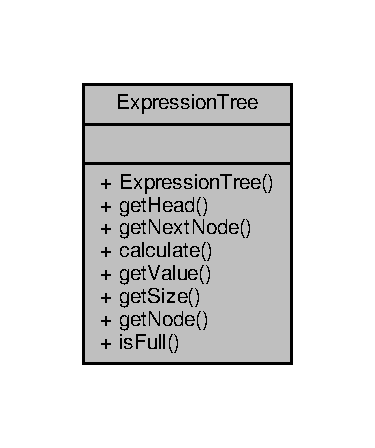
\includegraphics[width=180pt]{classExpressionTree__coll__graph}
\end{center}
\end{figure}
\subsection*{Public Member Functions}
\begin{DoxyCompactItemize}
\item 
\hyperlink{classExpressionNode}{Expression\+Node} $\ast$ {\bfseries get\+Head} ()\hypertarget{classExpressionTree_ad33a9486b731445db5b0a310ae1dccbc}{}\label{classExpressionTree_ad33a9486b731445db5b0a310ae1dccbc}

\item 
\hyperlink{classExpressionNode}{Expression\+Node} $\ast$ {\bfseries get\+Next\+Node} ()\hypertarget{classExpressionTree_a4c0be98d48d6a40bd0040e9ba6182da0}{}\label{classExpressionTree_a4c0be98d48d6a40bd0040e9ba6182da0}

\item 
void {\bfseries calculate} ()\hypertarget{classExpressionTree_a013e231688894895d6115947f51fc9ec}{}\label{classExpressionTree_a013e231688894895d6115947f51fc9ec}

\item 
int {\bfseries get\+Value} ()\hypertarget{classExpressionTree_aba1a8fe6a222342f2cc63fef28b6f3fc}{}\label{classExpressionTree_aba1a8fe6a222342f2cc63fef28b6f3fc}

\item 
int {\bfseries get\+Size} ()\hypertarget{classExpressionTree_a4c056d4c509602b0ec0bb230a4bcae57}{}\label{classExpressionTree_a4c056d4c509602b0ec0bb230a4bcae57}

\item 
\hyperlink{classExpressionNode}{Expression\+Node} $\ast$ {\bfseries get\+Node} (int index)\hypertarget{classExpressionTree_a249c0b529ab05f8b554b2b6d9002ce9b}{}\label{classExpressionTree_a249c0b529ab05f8b554b2b6d9002ce9b}

\item 
bool {\bfseries is\+Full} ()\hypertarget{classExpressionTree_af7bb11b664bd228c68ba81d557bc1f11}{}\label{classExpressionTree_af7bb11b664bd228c68ba81d557bc1f11}

\end{DoxyCompactItemize}


The documentation for this class was generated from the following files\+:\begin{DoxyCompactItemize}
\item 
/home/douglas/generator2/expressiontree.\+h\item 
/home/douglas/generator2/expressiontree.\+cpp\end{DoxyCompactItemize}

\hypertarget{classExpressionTreeFormatter}{}\section{Expression\+Tree\+Formatter Class Reference}
\label{classExpressionTreeFormatter}\index{Expression\+Tree\+Formatter@{Expression\+Tree\+Formatter}}


Inheritance diagram for Expression\+Tree\+Formatter\+:
\nopagebreak
\begin{figure}[H]
\begin{center}
\leavevmode
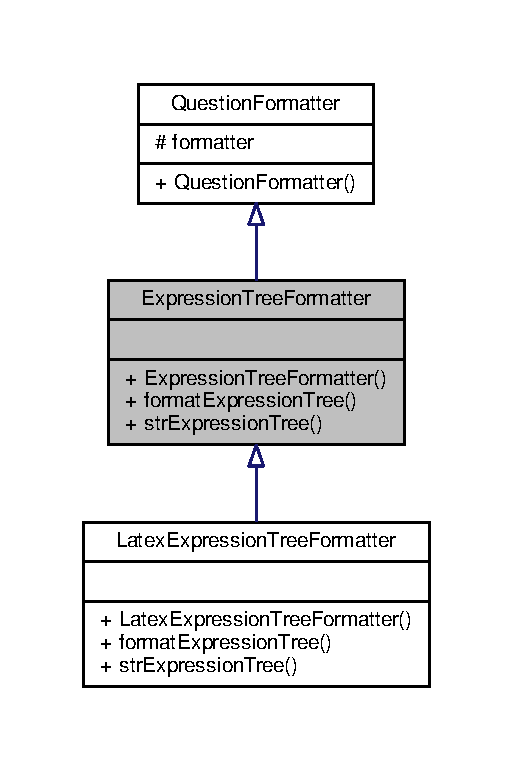
\includegraphics[width=246pt]{classExpressionTreeFormatter__inherit__graph}
\end{center}
\end{figure}


Collaboration diagram for Expression\+Tree\+Formatter\+:
\nopagebreak
\begin{figure}[H]
\begin{center}
\leavevmode
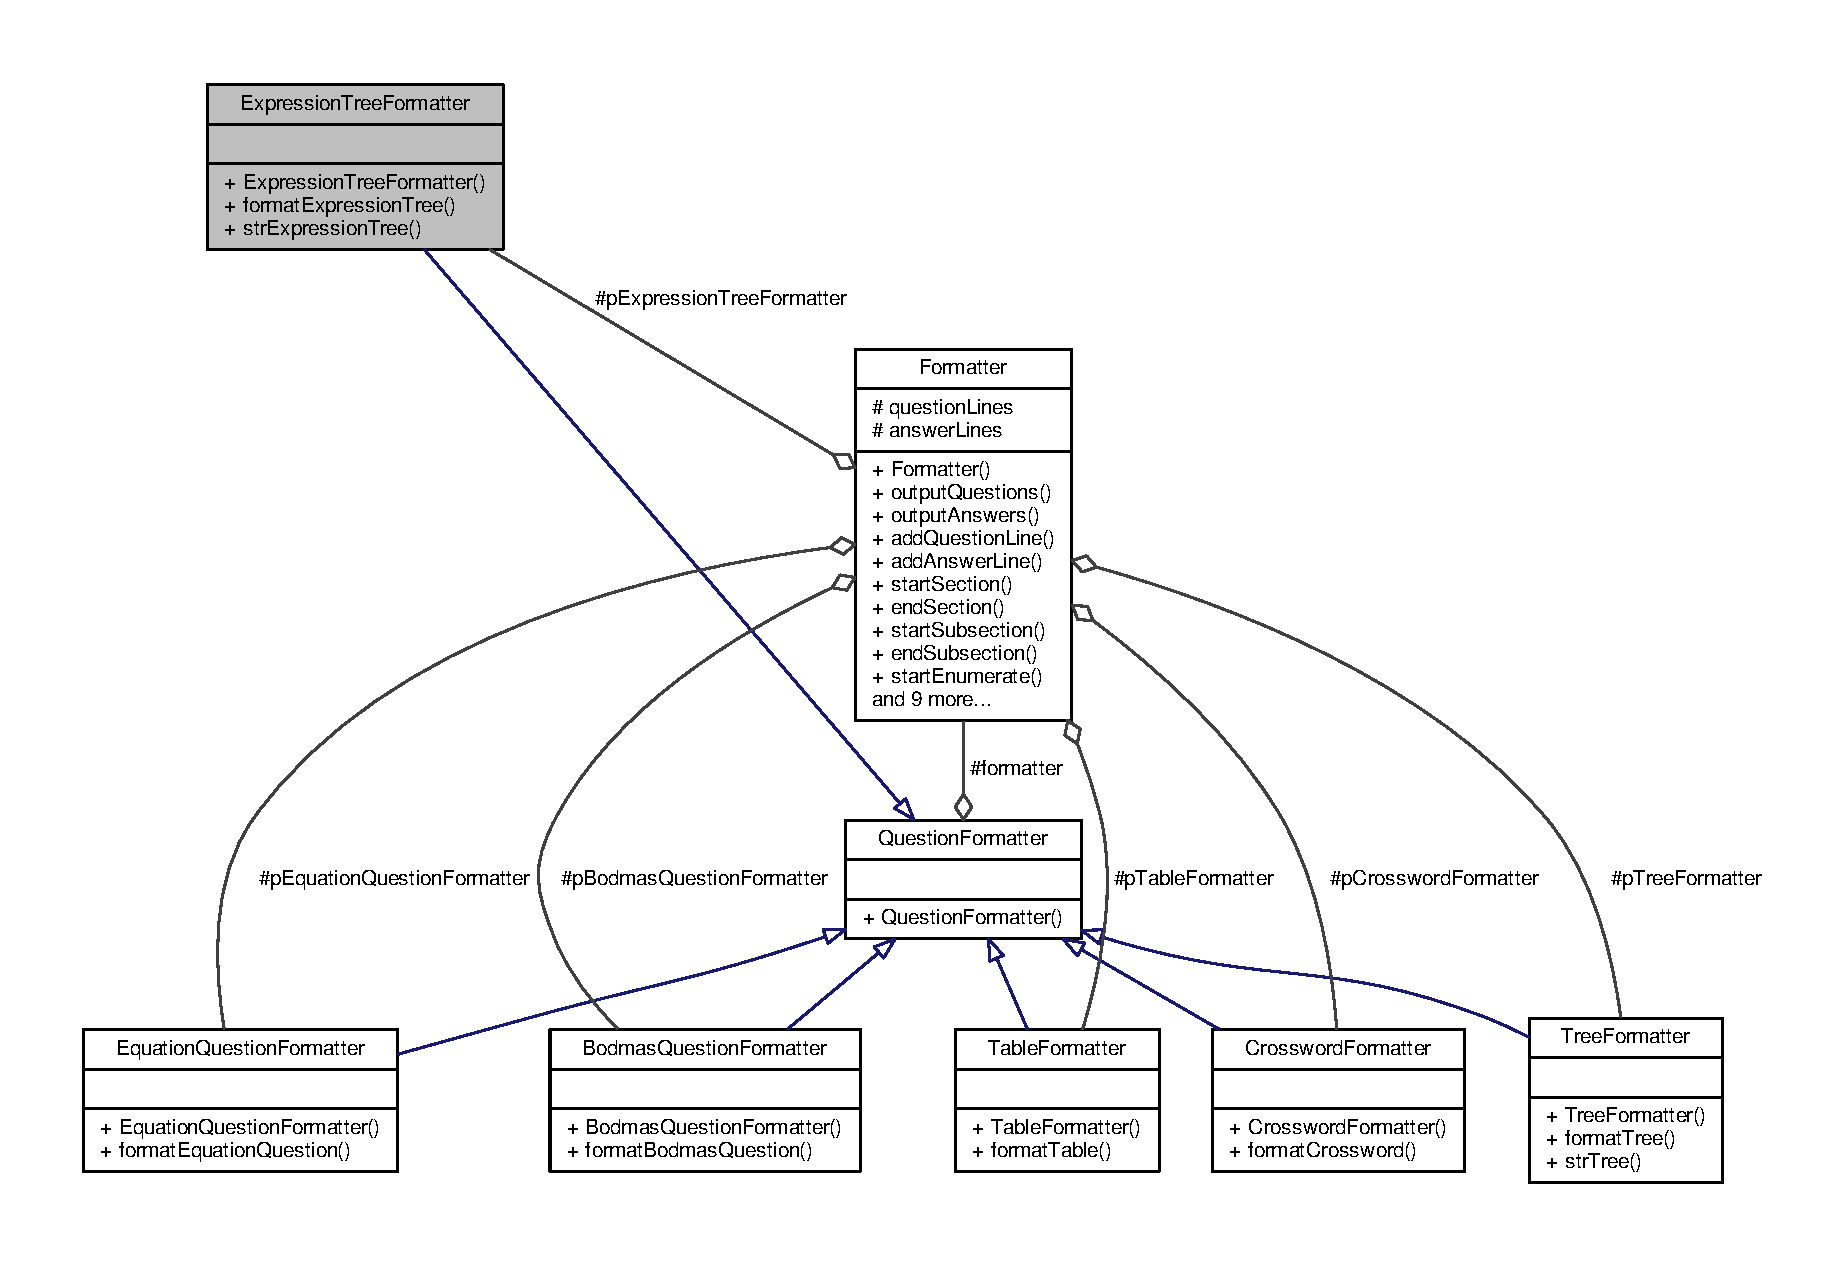
\includegraphics[width=350pt]{classExpressionTreeFormatter__coll__graph}
\end{center}
\end{figure}
\subsection*{Public Member Functions}
\begin{DoxyCompactItemize}
\item 
{\bfseries Expression\+Tree\+Formatter} (\hyperlink{classFormatter}{Formatter} $\ast$formatter)\hypertarget{classExpressionTreeFormatter_a5fc08300c831caac6e2a3194ef78d9c9}{}\label{classExpressionTreeFormatter_a5fc08300c831caac6e2a3194ef78d9c9}

\item 
virtual void {\bfseries format\+Expression\+Tree} (\hyperlink{classExpressionTree}{Expression\+Tree} $\ast$expression\+Tree)=0\hypertarget{classExpressionTreeFormatter_aeadc86b321a5ee4eac522cd8ebe04b00}{}\label{classExpressionTreeFormatter_aeadc86b321a5ee4eac522cd8ebe04b00}

\item 
virtual std\+::string {\bfseries str\+Expression\+Tree} (\hyperlink{classExpressionTree}{Expression\+Tree} $\ast$tree)=0\hypertarget{classExpressionTreeFormatter_a5e832a625b7c58016c76377d2ad9b9c5}{}\label{classExpressionTreeFormatter_a5e832a625b7c58016c76377d2ad9b9c5}

\end{DoxyCompactItemize}
\subsection*{Additional Inherited Members}


The documentation for this class was generated from the following files\+:\begin{DoxyCompactItemize}
\item 
/home/douglas/generator2/expressiontreeformatter.\+h\item 
/home/douglas/generator2/expressiontreeformatter.\+cpp\end{DoxyCompactItemize}

\hypertarget{classFactorFinder}{}\section{Factor\+Finder Class Reference}
\label{classFactorFinder}\index{Factor\+Finder@{Factor\+Finder}}


Collaboration diagram for Factor\+Finder\+:
\nopagebreak
\begin{figure}[H]
\begin{center}
\leavevmode
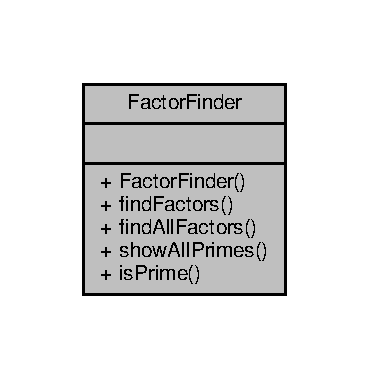
\includegraphics[width=177pt]{classFactorFinder__coll__graph}
\end{center}
\end{figure}
\subsection*{Public Member Functions}
\begin{DoxyCompactItemize}
\item 
void {\bfseries find\+Factors} (int number, int \&out\+FactorA, int \&out\+FactorB)\hypertarget{classFactorFinder_aab480bdfe42adc80d00390b10f453665}{}\label{classFactorFinder_aab480bdfe42adc80d00390b10f453665}

\item 
void {\bfseries find\+All\+Factors} (int number, std\+::vector$<$ int $>$ \&out\+Factor\+List)\hypertarget{classFactorFinder_a3482682d018ac13f6d67a5c35649dd5e}{}\label{classFactorFinder_a3482682d018ac13f6d67a5c35649dd5e}

\item 
void {\bfseries show\+All\+Primes} ()\hypertarget{classFactorFinder_af4530a2fc1067443eb4425867cc6c781}{}\label{classFactorFinder_af4530a2fc1067443eb4425867cc6c781}

\item 
bool {\bfseries is\+Prime} (int number)\hypertarget{classFactorFinder_a056c479dacb381b63cfd2a6e429219c1}{}\label{classFactorFinder_a056c479dacb381b63cfd2a6e429219c1}

\end{DoxyCompactItemize}


The documentation for this class was generated from the following files\+:\begin{DoxyCompactItemize}
\item 
/home/douglas/generator2/factorfinder.\+h\item 
/home/douglas/generator2/factorfinder.\+cpp\end{DoxyCompactItemize}

\hypertarget{classFileReader}{}\section{File\+Reader Class Reference}
\label{classFileReader}\index{File\+Reader@{File\+Reader}}


Collaboration diagram for File\+Reader\+:
\nopagebreak
\begin{figure}[H]
\begin{center}
\leavevmode
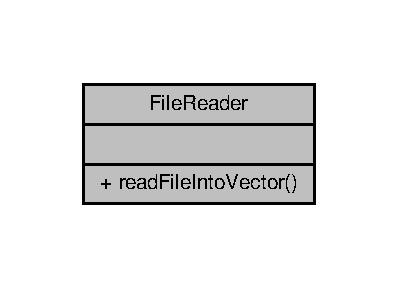
\includegraphics[width=191pt]{classFileReader__coll__graph}
\end{center}
\end{figure}
\subsection*{Public Member Functions}
\begin{DoxyCompactItemize}
\item 
void {\bfseries read\+File\+Into\+Vector} (const std\+::string filename, std\+::vector$<$ std\+::string $>$ \&string\+Vector)\hypertarget{classFileReader_a2479df28a04c08d003295a5dd0f698d3}{}\label{classFileReader_a2479df28a04c08d003295a5dd0f698d3}

\end{DoxyCompactItemize}


The documentation for this class was generated from the following files\+:\begin{DoxyCompactItemize}
\item 
/home/douglas/generator2/filereader.\+h\item 
/home/douglas/generator2/filereader.\+cpp\end{DoxyCompactItemize}

\hypertarget{classFormatter}{}\section{Formatter Class Reference}
\label{classFormatter}\index{Formatter@{Formatter}}


Inheritance diagram for Formatter\+:
\nopagebreak
\begin{figure}[H]
\begin{center}
\leavevmode
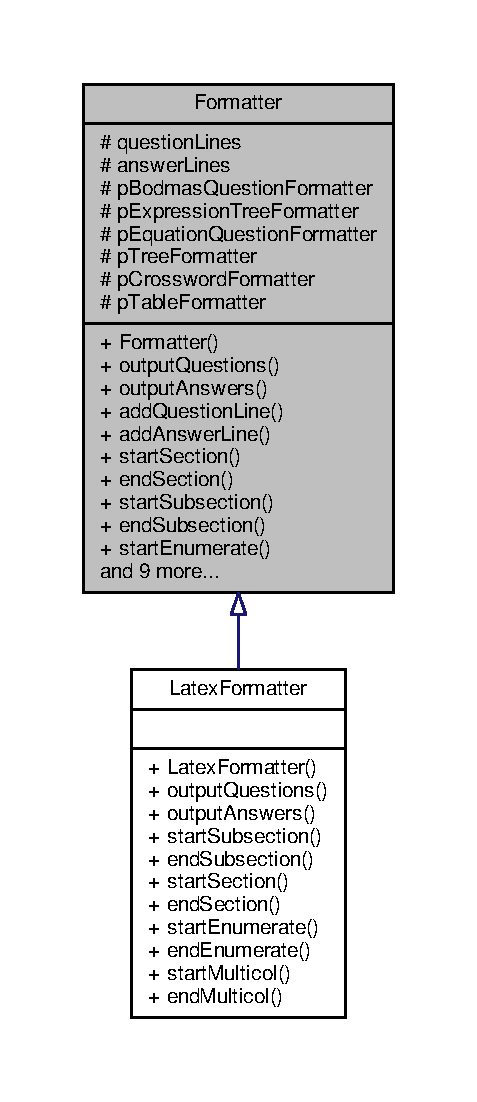
\includegraphics[width=229pt]{classFormatter__inherit__graph}
\end{center}
\end{figure}


Collaboration diagram for Formatter\+:
\nopagebreak
\begin{figure}[H]
\begin{center}
\leavevmode
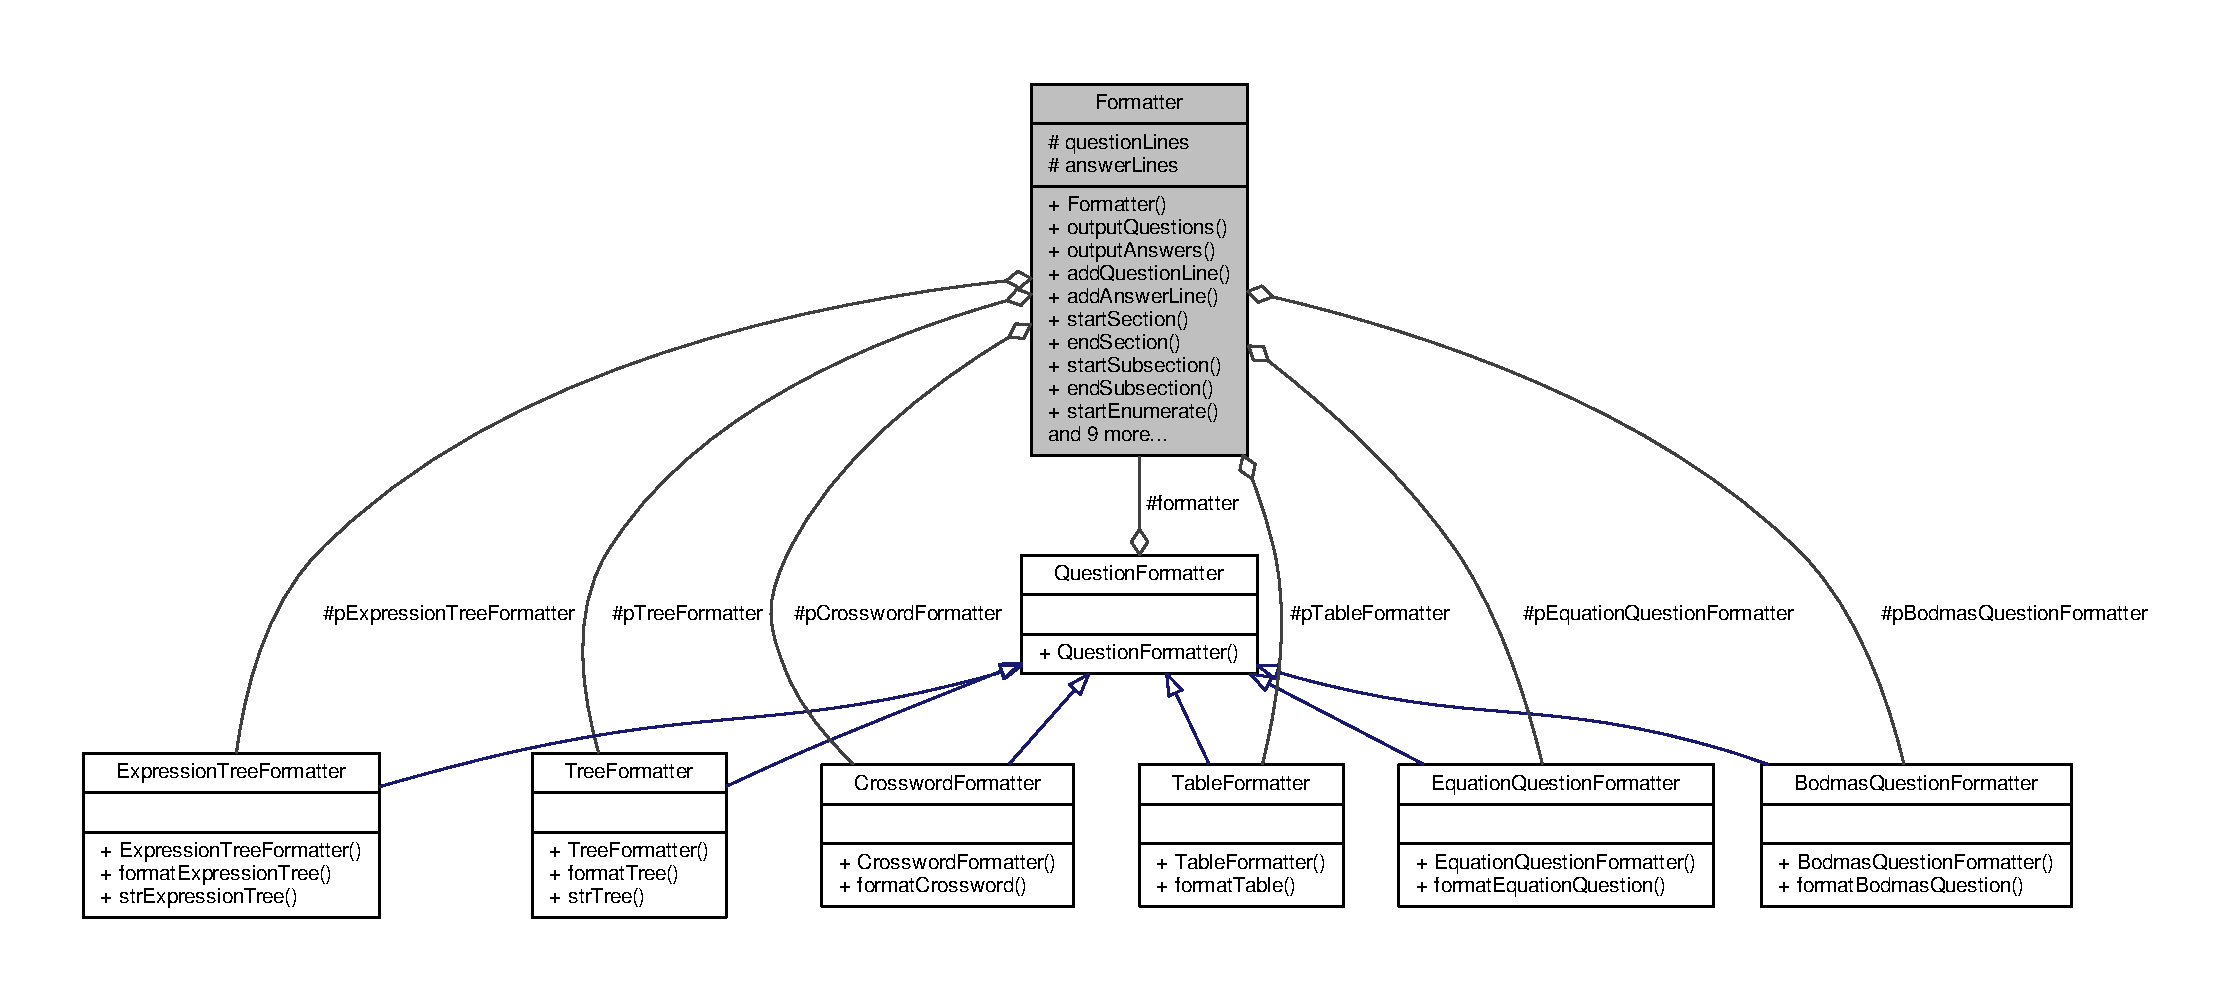
\includegraphics[width=350pt]{classFormatter__coll__graph}
\end{center}
\end{figure}
\subsection*{Public Member Functions}
\begin{DoxyCompactItemize}
\item 
virtual void {\bfseries output\+Questions} (std\+::ostream \&stream)=0\hypertarget{classFormatter_a98ff09fa6b041b352b11f52d314b0410}{}\label{classFormatter_a98ff09fa6b041b352b11f52d314b0410}

\item 
virtual void {\bfseries output\+Answers} (std\+::ostream \&stream)=0\hypertarget{classFormatter_a0fdcbe54f426fe453161682200e9bf48}{}\label{classFormatter_a0fdcbe54f426fe453161682200e9bf48}

\item 
void {\bfseries add\+Question\+Line} (const std\+::string line)\hypertarget{classFormatter_aba80ae3dd4e98f9e277977ef7ef61774}{}\label{classFormatter_aba80ae3dd4e98f9e277977ef7ef61774}

\item 
void {\bfseries add\+Answer\+Line} (const std\+::string line)\hypertarget{classFormatter_adebd4aa432d008191ef03b475a267056}{}\label{classFormatter_adebd4aa432d008191ef03b475a267056}

\item 
virtual void {\bfseries start\+Section} (const std\+::string section\+Name)=0\hypertarget{classFormatter_afadeabc0c5b4b6bd048ef3f730a695ca}{}\label{classFormatter_afadeabc0c5b4b6bd048ef3f730a695ca}

\item 
virtual void {\bfseries end\+Section} ()=0\hypertarget{classFormatter_a2004debe52f66791be806d07e701bbc4}{}\label{classFormatter_a2004debe52f66791be806d07e701bbc4}

\item 
virtual void {\bfseries start\+Subsection} (const std\+::string section\+Name)=0\hypertarget{classFormatter_a8a6e1379a7d2ecb4e44901afc08a5323}{}\label{classFormatter_a8a6e1379a7d2ecb4e44901afc08a5323}

\item 
virtual void {\bfseries end\+Subsection} ()=0\hypertarget{classFormatter_ae91cf6f493111f5bc6fc9ffbf6d4e6f2}{}\label{classFormatter_ae91cf6f493111f5bc6fc9ffbf6d4e6f2}

\item 
virtual void {\bfseries start\+Enumerate} ()=0\hypertarget{classFormatter_aba4c98ea2a0a7613bd15bd279a7509e5}{}\label{classFormatter_aba4c98ea2a0a7613bd15bd279a7509e5}

\item 
virtual void {\bfseries end\+Enumerate} ()=0\hypertarget{classFormatter_ae618eab17049dee40305b2d989828e8c}{}\label{classFormatter_ae618eab17049dee40305b2d989828e8c}

\item 
virtual void {\bfseries start\+Multicol} (int num\+Columns)=0\hypertarget{classFormatter_a7cf2ea87ddf2bf145e0b1aab77783b9f}{}\label{classFormatter_a7cf2ea87ddf2bf145e0b1aab77783b9f}

\item 
virtual void {\bfseries end\+Multicol} ()=0\hypertarget{classFormatter_a54f2ad368afbd1ebe2756ff2b3c1dc07}{}\label{classFormatter_a54f2ad368afbd1ebe2756ff2b3c1dc07}

\item 
\hyperlink{classBodmasQuestionFormatter}{Bodmas\+Question\+Formatter} $\ast$ {\bfseries get\+Bodmas\+Question\+Formatter} ()\hypertarget{classFormatter_a98e1fd8588a6f54f0d5f0d0ce13e2960}{}\label{classFormatter_a98e1fd8588a6f54f0d5f0d0ce13e2960}

\item 
\hyperlink{classExpressionTreeFormatter}{Expression\+Tree\+Formatter} $\ast$ {\bfseries get\+Expression\+Tree\+Formatter} ()\hypertarget{classFormatter_ab5aecec4b4cbe567ca208f355d546115}{}\label{classFormatter_ab5aecec4b4cbe567ca208f355d546115}

\item 
\hyperlink{classEquationQuestionFormatter}{Equation\+Question\+Formatter} $\ast$ {\bfseries get\+Equation\+Question\+Formatter} ()\hypertarget{classFormatter_a3a2f3fb9176ec9b50d86822381c06a64}{}\label{classFormatter_a3a2f3fb9176ec9b50d86822381c06a64}

\item 
\hyperlink{classTreeFormatter}{Tree\+Formatter} $\ast$ {\bfseries get\+Tree\+Formatter} ()\hypertarget{classFormatter_ac5f9b6234b04f0017a80fd4e74a812d9}{}\label{classFormatter_ac5f9b6234b04f0017a80fd4e74a812d9}

\item 
\hyperlink{classCrosswordFormatter}{Crossword\+Formatter} $\ast$ {\bfseries get\+Crossword\+Formatter} ()\hypertarget{classFormatter_a513014a14b51125c6440dcf46de5386d}{}\label{classFormatter_a513014a14b51125c6440dcf46de5386d}

\item 
\hyperlink{classTableFormatter}{Table\+Formatter} $\ast$ {\bfseries get\+Table\+Formatter} ()\hypertarget{classFormatter_a52ef285118fe34628af60c5ff55cfafc}{}\label{classFormatter_a52ef285118fe34628af60c5ff55cfafc}

\end{DoxyCompactItemize}
\subsection*{Protected Attributes}
\begin{DoxyCompactItemize}
\item 
std\+::vector$<$ std\+::string $>$ {\bfseries question\+Lines}\hypertarget{classFormatter_abe848f063503f3587b1a83ad82df7c1e}{}\label{classFormatter_abe848f063503f3587b1a83ad82df7c1e}

\item 
std\+::vector$<$ std\+::string $>$ {\bfseries answer\+Lines}\hypertarget{classFormatter_ab2cdeb8cdcad98582233117f071d559e}{}\label{classFormatter_ab2cdeb8cdcad98582233117f071d559e}

\item 
\hyperlink{classBodmasQuestionFormatter}{Bodmas\+Question\+Formatter} $\ast$ {\bfseries p\+Bodmas\+Question\+Formatter}\hypertarget{classFormatter_a310eae52988f88652fc6f5dbf663e6d4}{}\label{classFormatter_a310eae52988f88652fc6f5dbf663e6d4}

\item 
\hyperlink{classExpressionTreeFormatter}{Expression\+Tree\+Formatter} $\ast$ {\bfseries p\+Expression\+Tree\+Formatter}\hypertarget{classFormatter_a31bd119c1109ccfdec1024775414094e}{}\label{classFormatter_a31bd119c1109ccfdec1024775414094e}

\item 
\hyperlink{classEquationQuestionFormatter}{Equation\+Question\+Formatter} $\ast$ {\bfseries p\+Equation\+Question\+Formatter}\hypertarget{classFormatter_a1d44637895cb280cc04e12cfebeb2b0a}{}\label{classFormatter_a1d44637895cb280cc04e12cfebeb2b0a}

\item 
\hyperlink{classTreeFormatter}{Tree\+Formatter} $\ast$ {\bfseries p\+Tree\+Formatter}\hypertarget{classFormatter_a7a0449140b074f4918f1235657eca242}{}\label{classFormatter_a7a0449140b074f4918f1235657eca242}

\item 
\hyperlink{classCrosswordFormatter}{Crossword\+Formatter} $\ast$ {\bfseries p\+Crossword\+Formatter}\hypertarget{classFormatter_ae3237e47677e1ed9da3dea4d912b4a3c}{}\label{classFormatter_ae3237e47677e1ed9da3dea4d912b4a3c}

\item 
\hyperlink{classTableFormatter}{Table\+Formatter} $\ast$ {\bfseries p\+Table\+Formatter}\hypertarget{classFormatter_a7919aa24002409a139d7b6730630ab86}{}\label{classFormatter_a7919aa24002409a139d7b6730630ab86}

\end{DoxyCompactItemize}


The documentation for this class was generated from the following files\+:\begin{DoxyCompactItemize}
\item 
/home/douglas/generator2/formatter.\+h\item 
/home/douglas/generator2/formatter.\+cpp\end{DoxyCompactItemize}

\hypertarget{classFormula}{}\section{Formula Class Reference}
\label{classFormula}\index{Formula@{Formula}}


Collaboration diagram for Formula\+:
\nopagebreak
\begin{figure}[H]
\begin{center}
\leavevmode
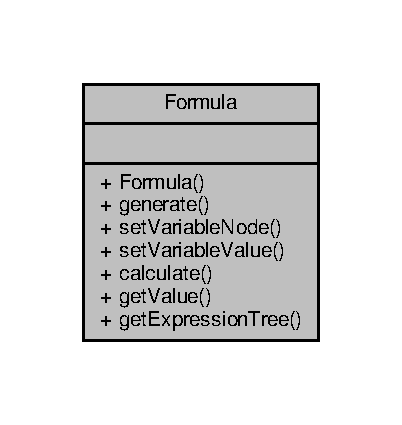
\includegraphics[width=193pt]{classFormula__coll__graph}
\end{center}
\end{figure}
\subsection*{Public Member Functions}
\begin{DoxyCompactItemize}
\item 
void {\bfseries generate} (std\+::vector$<$ std\+::string $>$ \&args)\hypertarget{classFormula_aae68f090a158b164ddbb46158e411c54}{}\label{classFormula_aae68f090a158b164ddbb46158e411c54}

\item 
void {\bfseries set\+Variable\+Node} (\hyperlink{classExpressionNode}{Expression\+Node} $\ast$node, char variable)\hypertarget{classFormula_ac6bbb91048c27c3aa69aa8731459b6fd}{}\label{classFormula_ac6bbb91048c27c3aa69aa8731459b6fd}

\item 
void {\bfseries set\+Variable\+Value} (char variable, int value)\hypertarget{classFormula_acc23e4da57c36e2ed75e698ddf77a409}{}\label{classFormula_acc23e4da57c36e2ed75e698ddf77a409}

\item 
void {\bfseries calculate} ()\hypertarget{classFormula_a031a0080a041ebf11c7364059decceca}{}\label{classFormula_a031a0080a041ebf11c7364059decceca}

\item 
int {\bfseries get\+Value} ()\hypertarget{classFormula_a00d976580373a7b44ca0ce4304e404db}{}\label{classFormula_a00d976580373a7b44ca0ce4304e404db}

\item 
\hyperlink{classExpressionTree}{Expression\+Tree} \& {\bfseries get\+Expression\+Tree} ()\hypertarget{classFormula_a2ba89fba606ca10a22f3936601da2f60}{}\label{classFormula_a2ba89fba606ca10a22f3936601da2f60}

\end{DoxyCompactItemize}


The documentation for this class was generated from the following files\+:\begin{DoxyCompactItemize}
\item 
/home/douglas/generator2/formula.\+h\item 
/home/douglas/generator2/formula.\+cpp\end{DoxyCompactItemize}

\hypertarget{classLatexBodmasQuestionFormatter}{}\section{Latex\+Bodmas\+Question\+Formatter Class Reference}
\label{classLatexBodmasQuestionFormatter}\index{Latex\+Bodmas\+Question\+Formatter@{Latex\+Bodmas\+Question\+Formatter}}


Inheritance diagram for Latex\+Bodmas\+Question\+Formatter\+:
\nopagebreak
\begin{figure}[H]
\begin{center}
\leavevmode
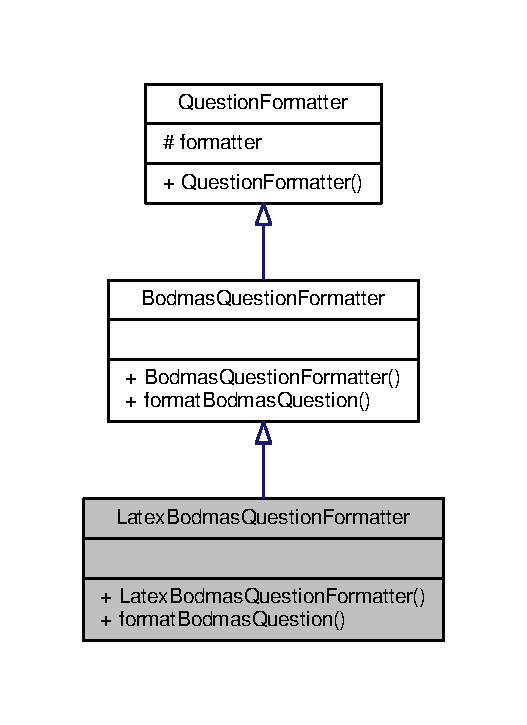
\includegraphics[width=253pt]{classLatexBodmasQuestionFormatter__inherit__graph}
\end{center}
\end{figure}


Collaboration diagram for Latex\+Bodmas\+Question\+Formatter\+:
\nopagebreak
\begin{figure}[H]
\begin{center}
\leavevmode
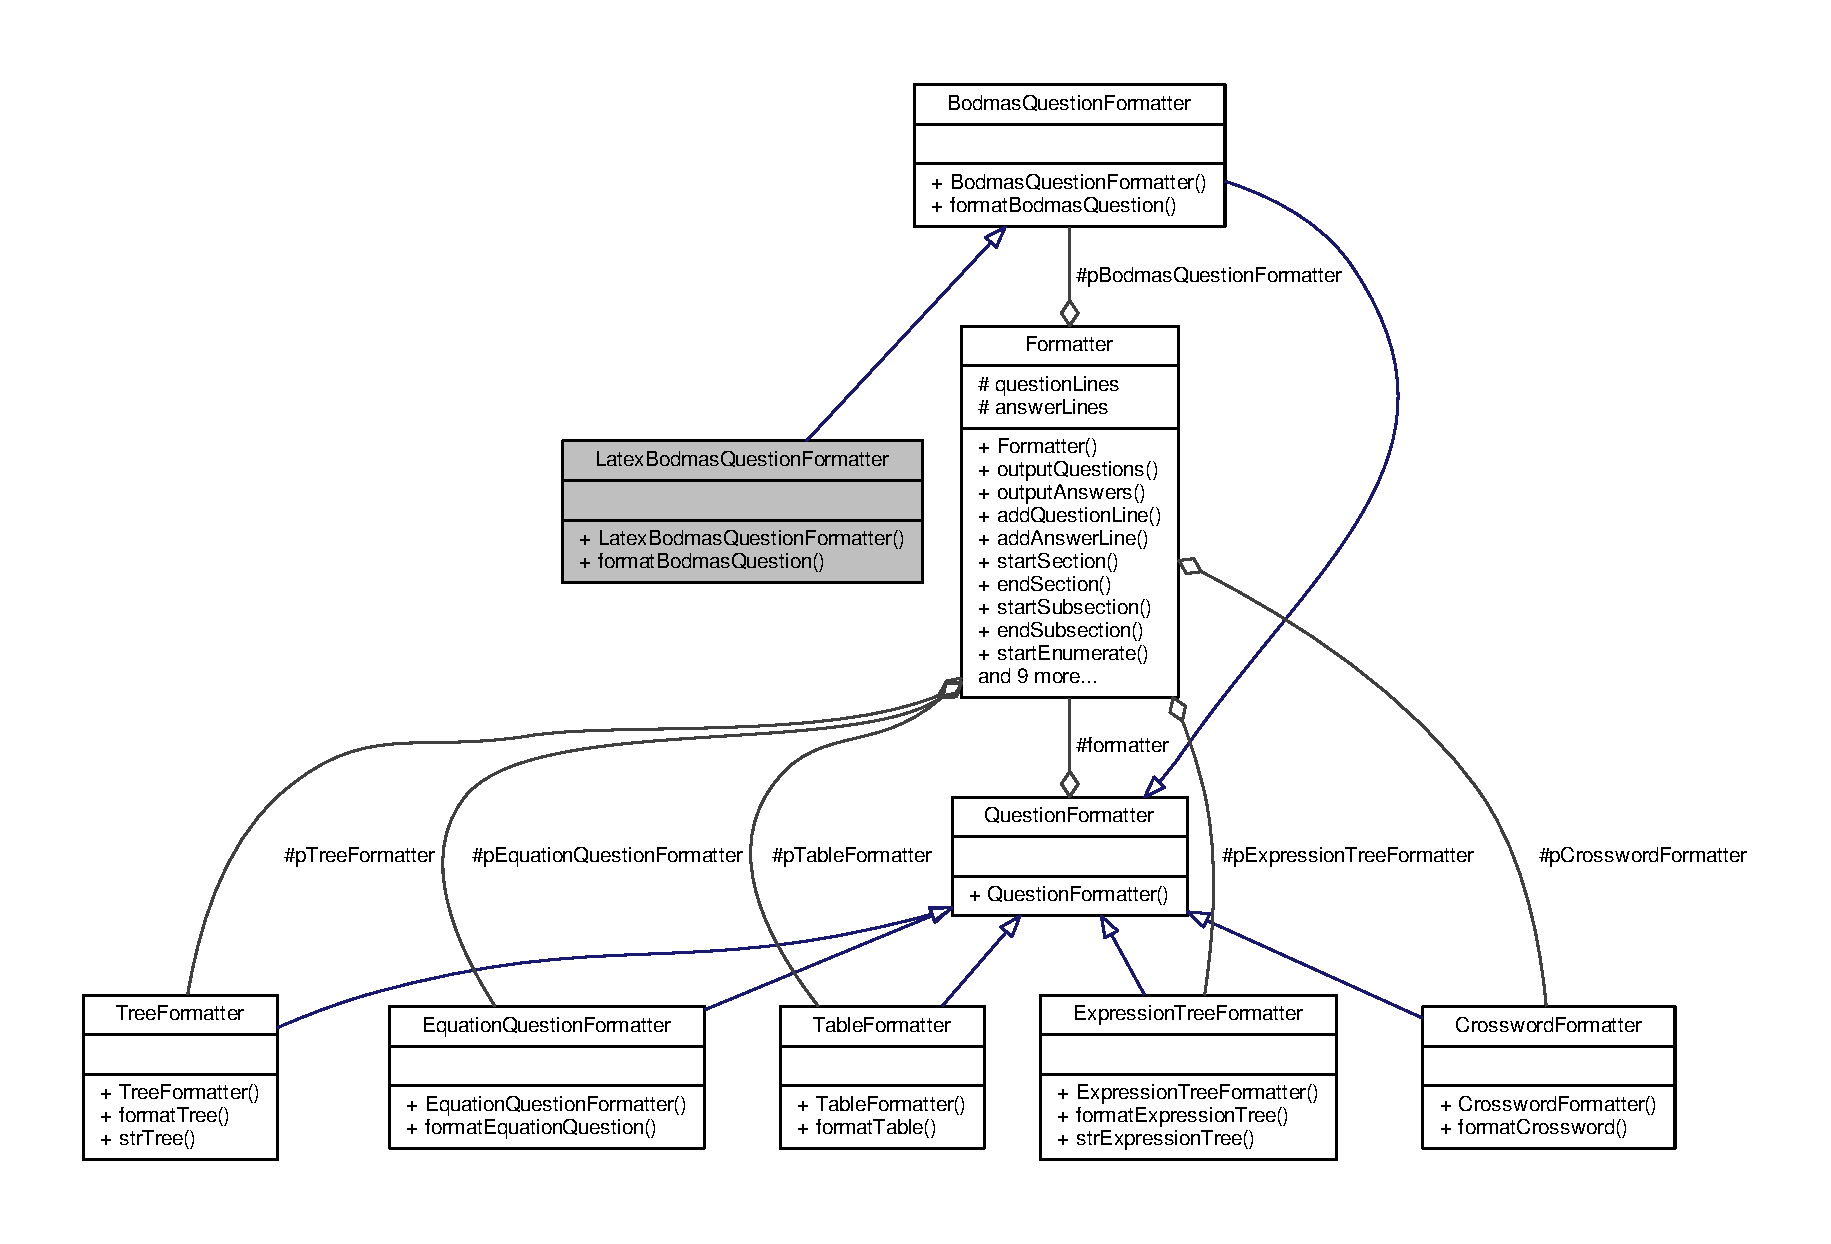
\includegraphics[width=350pt]{classLatexBodmasQuestionFormatter__coll__graph}
\end{center}
\end{figure}
\subsection*{Public Member Functions}
\begin{DoxyCompactItemize}
\item 
{\bfseries Latex\+Bodmas\+Question\+Formatter} (\hyperlink{classFormatter}{Formatter} $\ast$formatter)\hypertarget{classLatexBodmasQuestionFormatter_add7c9fceefb8c9e4aaf48c814199e3b8}{}\label{classLatexBodmasQuestionFormatter_add7c9fceefb8c9e4aaf48c814199e3b8}

\item 
virtual void {\bfseries format\+Bodmas\+Question} (\hyperlink{classBodmasQuestion}{Bodmas\+Question} $\ast$question)\hypertarget{classLatexBodmasQuestionFormatter_a0728ef69d83fa548ed4f3084bb1c5897}{}\label{classLatexBodmasQuestionFormatter_a0728ef69d83fa548ed4f3084bb1c5897}

\end{DoxyCompactItemize}
\subsection*{Additional Inherited Members}


The documentation for this class was generated from the following files\+:\begin{DoxyCompactItemize}
\item 
/home/douglas/generator2/latexbodmasquestionformatter.\+h\item 
/home/douglas/generator2/latexbodmasquestionformatter.\+cpp\end{DoxyCompactItemize}

\hypertarget{classLatexCrosswordFormatter}{}\section{Latex\+Crossword\+Formatter Class Reference}
\label{classLatexCrosswordFormatter}\index{Latex\+Crossword\+Formatter@{Latex\+Crossword\+Formatter}}


Inheritance diagram for Latex\+Crossword\+Formatter\+:
\nopagebreak
\begin{figure}[H]
\begin{center}
\leavevmode
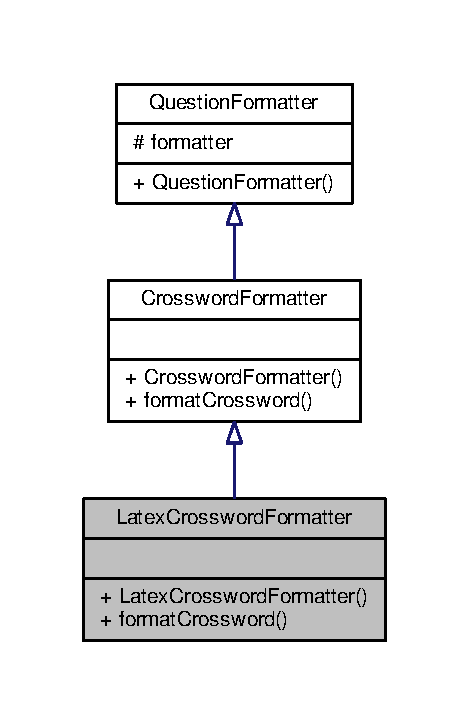
\includegraphics[width=225pt]{classLatexCrosswordFormatter__inherit__graph}
\end{center}
\end{figure}


Collaboration diagram for Latex\+Crossword\+Formatter\+:
\nopagebreak
\begin{figure}[H]
\begin{center}
\leavevmode
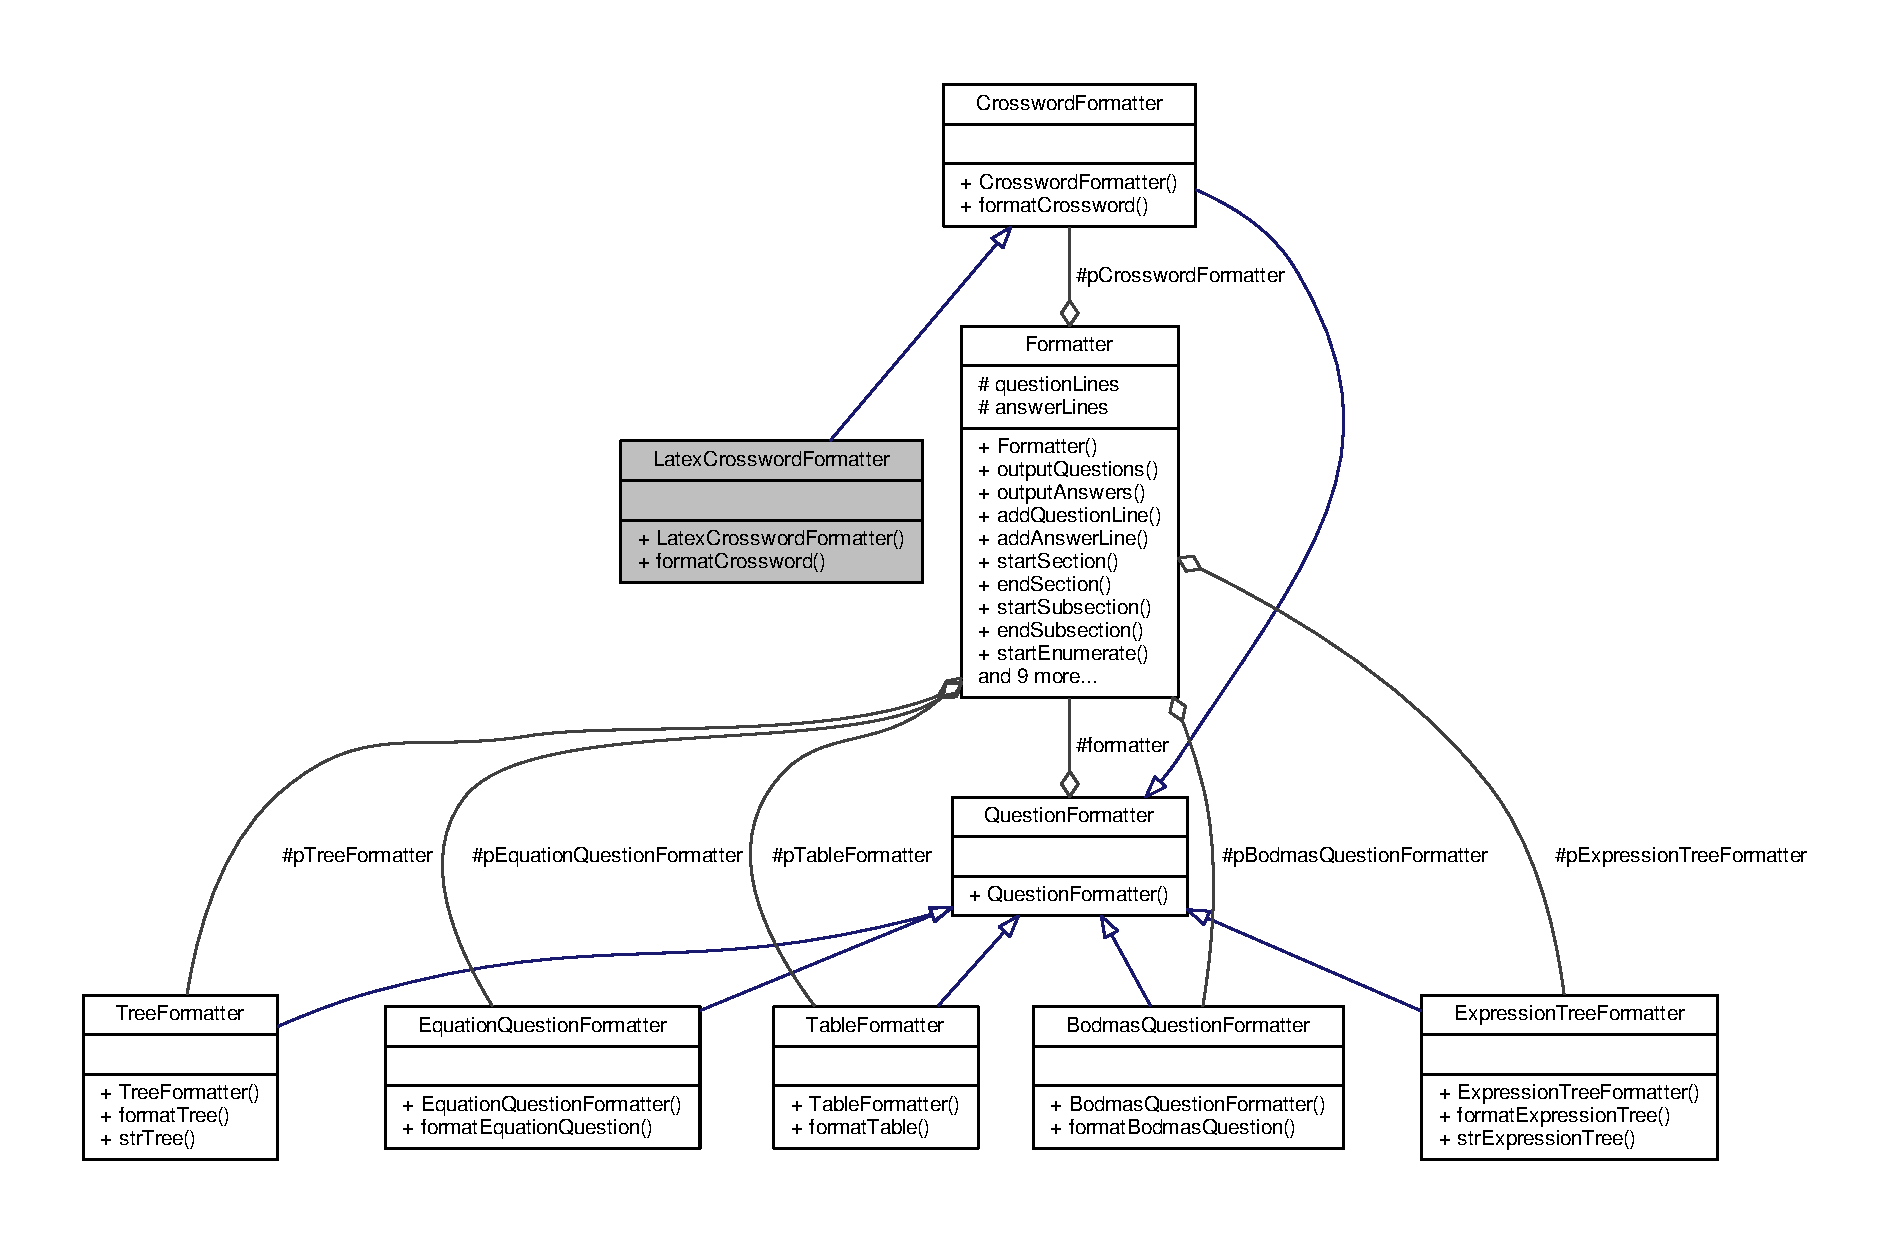
\includegraphics[width=350pt]{classLatexCrosswordFormatter__coll__graph}
\end{center}
\end{figure}
\subsection*{Public Member Functions}
\begin{DoxyCompactItemize}
\item 
{\bfseries Latex\+Crossword\+Formatter} (\hyperlink{classFormatter}{Formatter} $\ast$formatter)\hypertarget{classLatexCrosswordFormatter_a7cdcf1ef94e921bed033a3cc56131ee9}{}\label{classLatexCrosswordFormatter_a7cdcf1ef94e921bed033a3cc56131ee9}

\item 
virtual void {\bfseries format\+Crossword} (\hyperlink{classCrossword}{Crossword} $\ast$crossword)\hypertarget{classLatexCrosswordFormatter_a91a60b95a134485842962bac1f4b8753}{}\label{classLatexCrosswordFormatter_a91a60b95a134485842962bac1f4b8753}

\end{DoxyCompactItemize}
\subsection*{Additional Inherited Members}


The documentation for this class was generated from the following files\+:\begin{DoxyCompactItemize}
\item 
/home/douglas/generator2/latexcrosswordformatter.\+h\item 
/home/douglas/generator2/latexcrosswordformatter.\+cpp\end{DoxyCompactItemize}

\hypertarget{classLatexEquationQuestionFormatter}{}\section{Latex\+Equation\+Question\+Formatter Class Reference}
\label{classLatexEquationQuestionFormatter}\index{Latex\+Equation\+Question\+Formatter@{Latex\+Equation\+Question\+Formatter}}


Inheritance diagram for Latex\+Equation\+Question\+Formatter\+:
\nopagebreak
\begin{figure}[H]
\begin{center}
\leavevmode
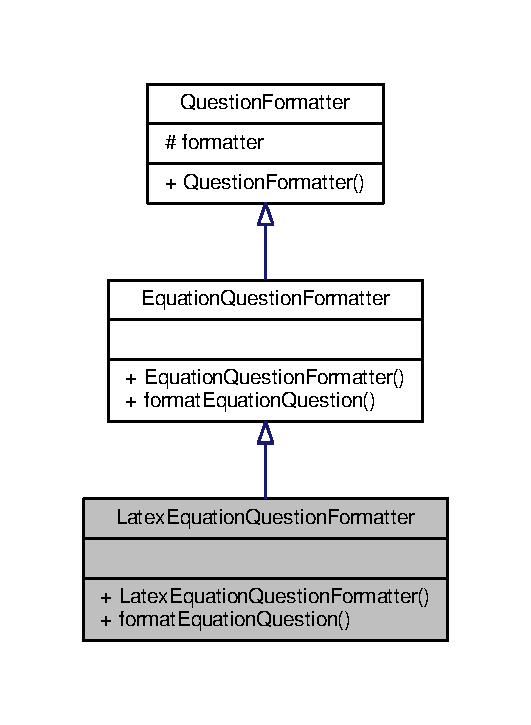
\includegraphics[width=255pt]{classLatexEquationQuestionFormatter__inherit__graph}
\end{center}
\end{figure}


Collaboration diagram for Latex\+Equation\+Question\+Formatter\+:
\nopagebreak
\begin{figure}[H]
\begin{center}
\leavevmode
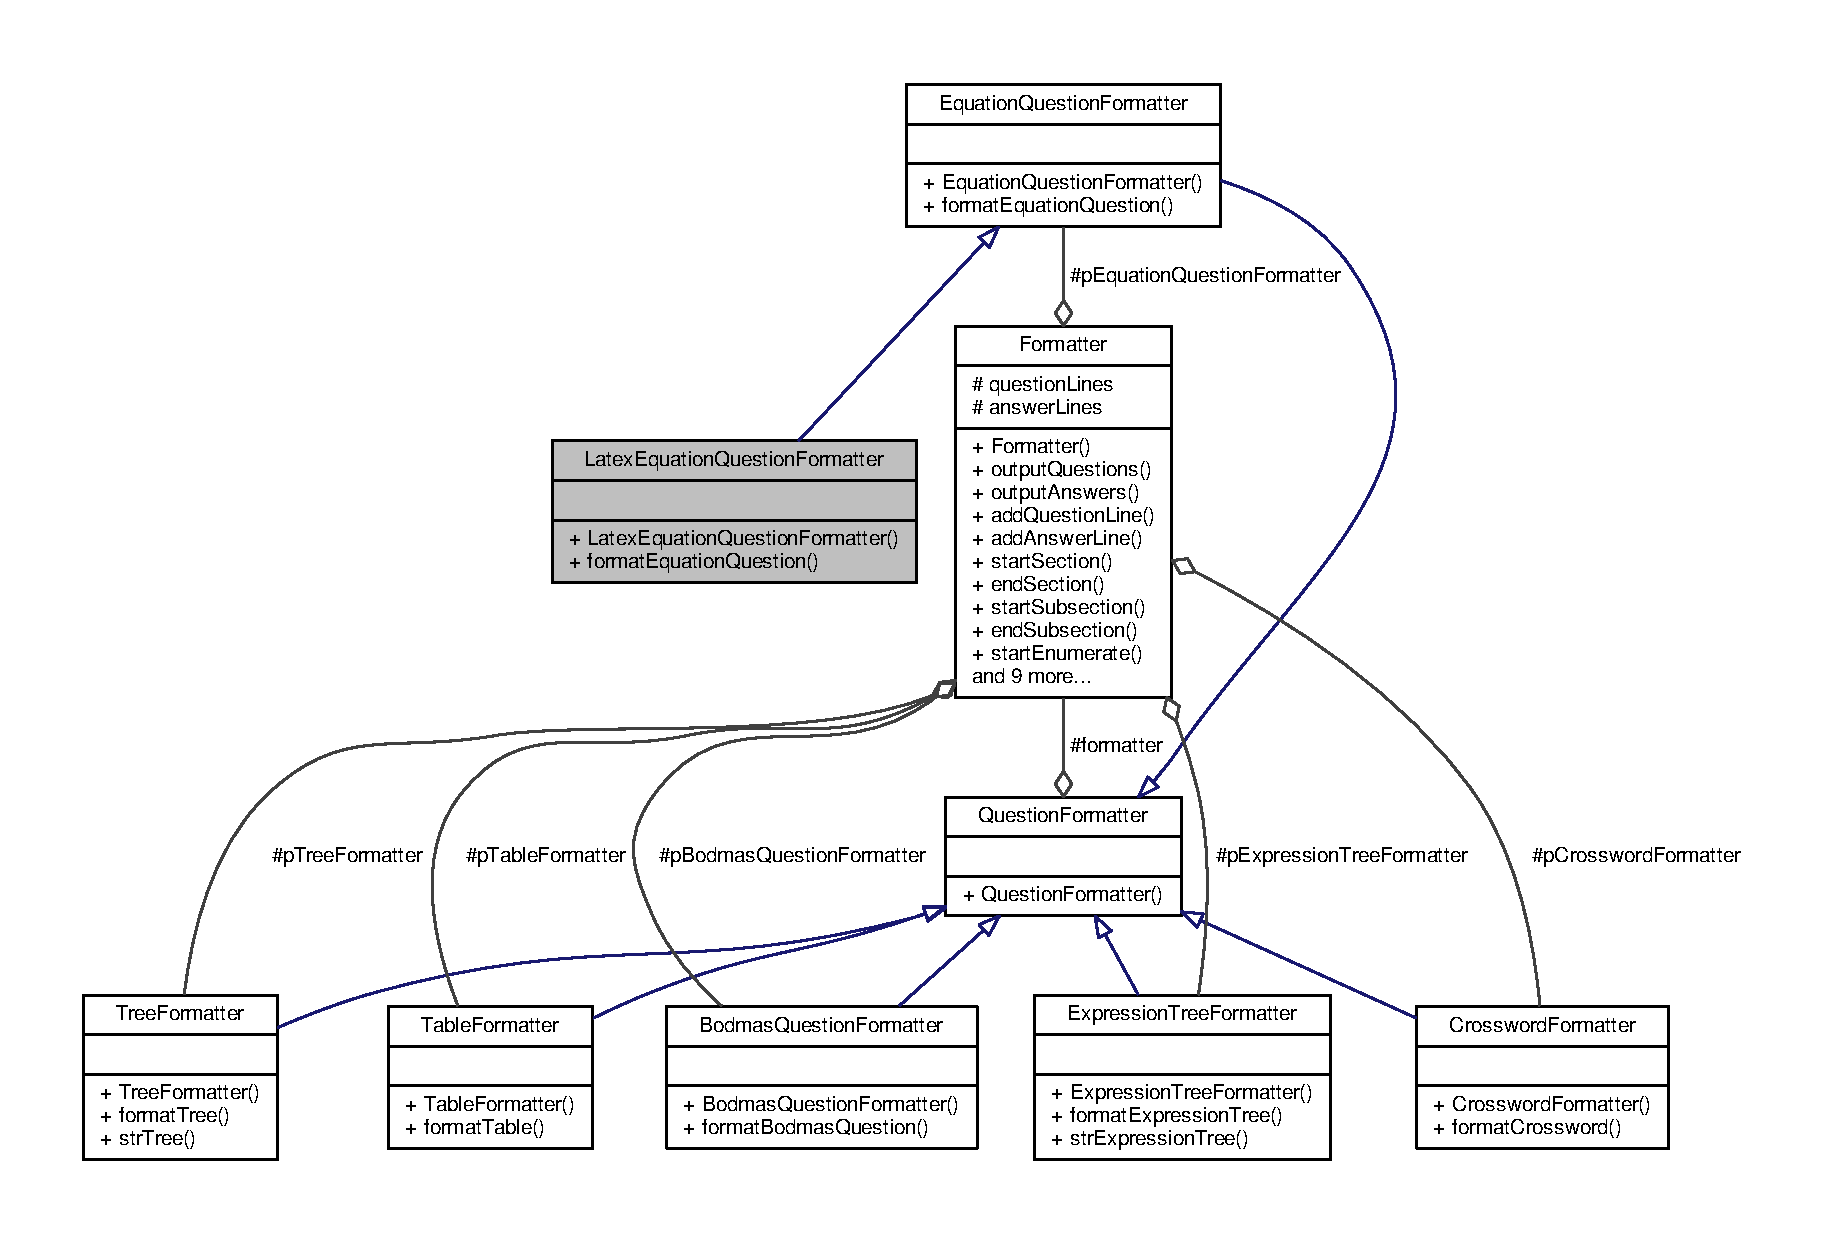
\includegraphics[width=350pt]{classLatexEquationQuestionFormatter__coll__graph}
\end{center}
\end{figure}
\subsection*{Public Member Functions}
\begin{DoxyCompactItemize}
\item 
{\bfseries Latex\+Equation\+Question\+Formatter} (\hyperlink{classFormatter}{Formatter} $\ast$formatter)\hypertarget{classLatexEquationQuestionFormatter_abfc56460ec6befbb189b57f338513a4d}{}\label{classLatexEquationQuestionFormatter_abfc56460ec6befbb189b57f338513a4d}

\item 
virtual void {\bfseries format\+Equation\+Question} (\hyperlink{classEquationQuestion}{Equation\+Question} $\ast$question)\hypertarget{classLatexEquationQuestionFormatter_a8051f09e7bf9a8aeb732a49f7299c9cf}{}\label{classLatexEquationQuestionFormatter_a8051f09e7bf9a8aeb732a49f7299c9cf}

\end{DoxyCompactItemize}
\subsection*{Additional Inherited Members}


The documentation for this class was generated from the following files\+:\begin{DoxyCompactItemize}
\item 
/home/douglas/generator2/latexequationquestionformatter.\+h\item 
/home/douglas/generator2/latexequationquestionformatter.\+cpp\end{DoxyCompactItemize}

\hypertarget{classLatexExpressionTreeFormatter}{}\section{Latex\+Expression\+Tree\+Formatter Class Reference}
\label{classLatexExpressionTreeFormatter}\index{Latex\+Expression\+Tree\+Formatter@{Latex\+Expression\+Tree\+Formatter}}


Inheritance diagram for Latex\+Expression\+Tree\+Formatter\+:
\nopagebreak
\begin{figure}[H]
\begin{center}
\leavevmode
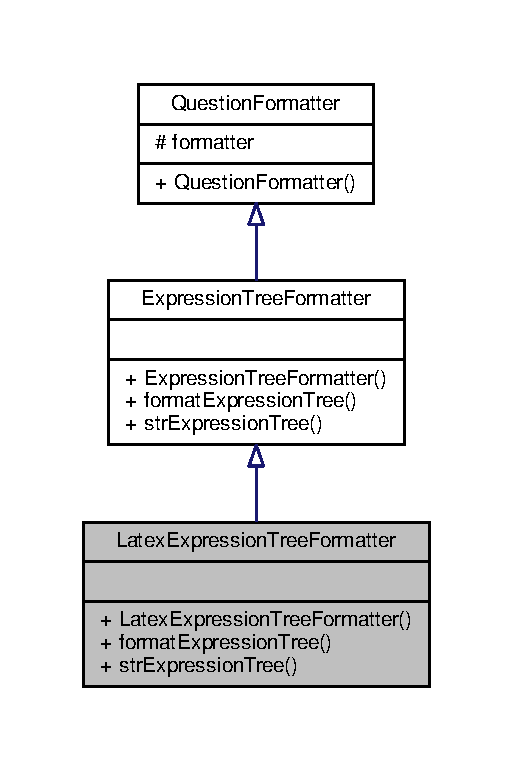
\includegraphics[width=246pt]{classLatexExpressionTreeFormatter__inherit__graph}
\end{center}
\end{figure}


Collaboration diagram for Latex\+Expression\+Tree\+Formatter\+:
\nopagebreak
\begin{figure}[H]
\begin{center}
\leavevmode
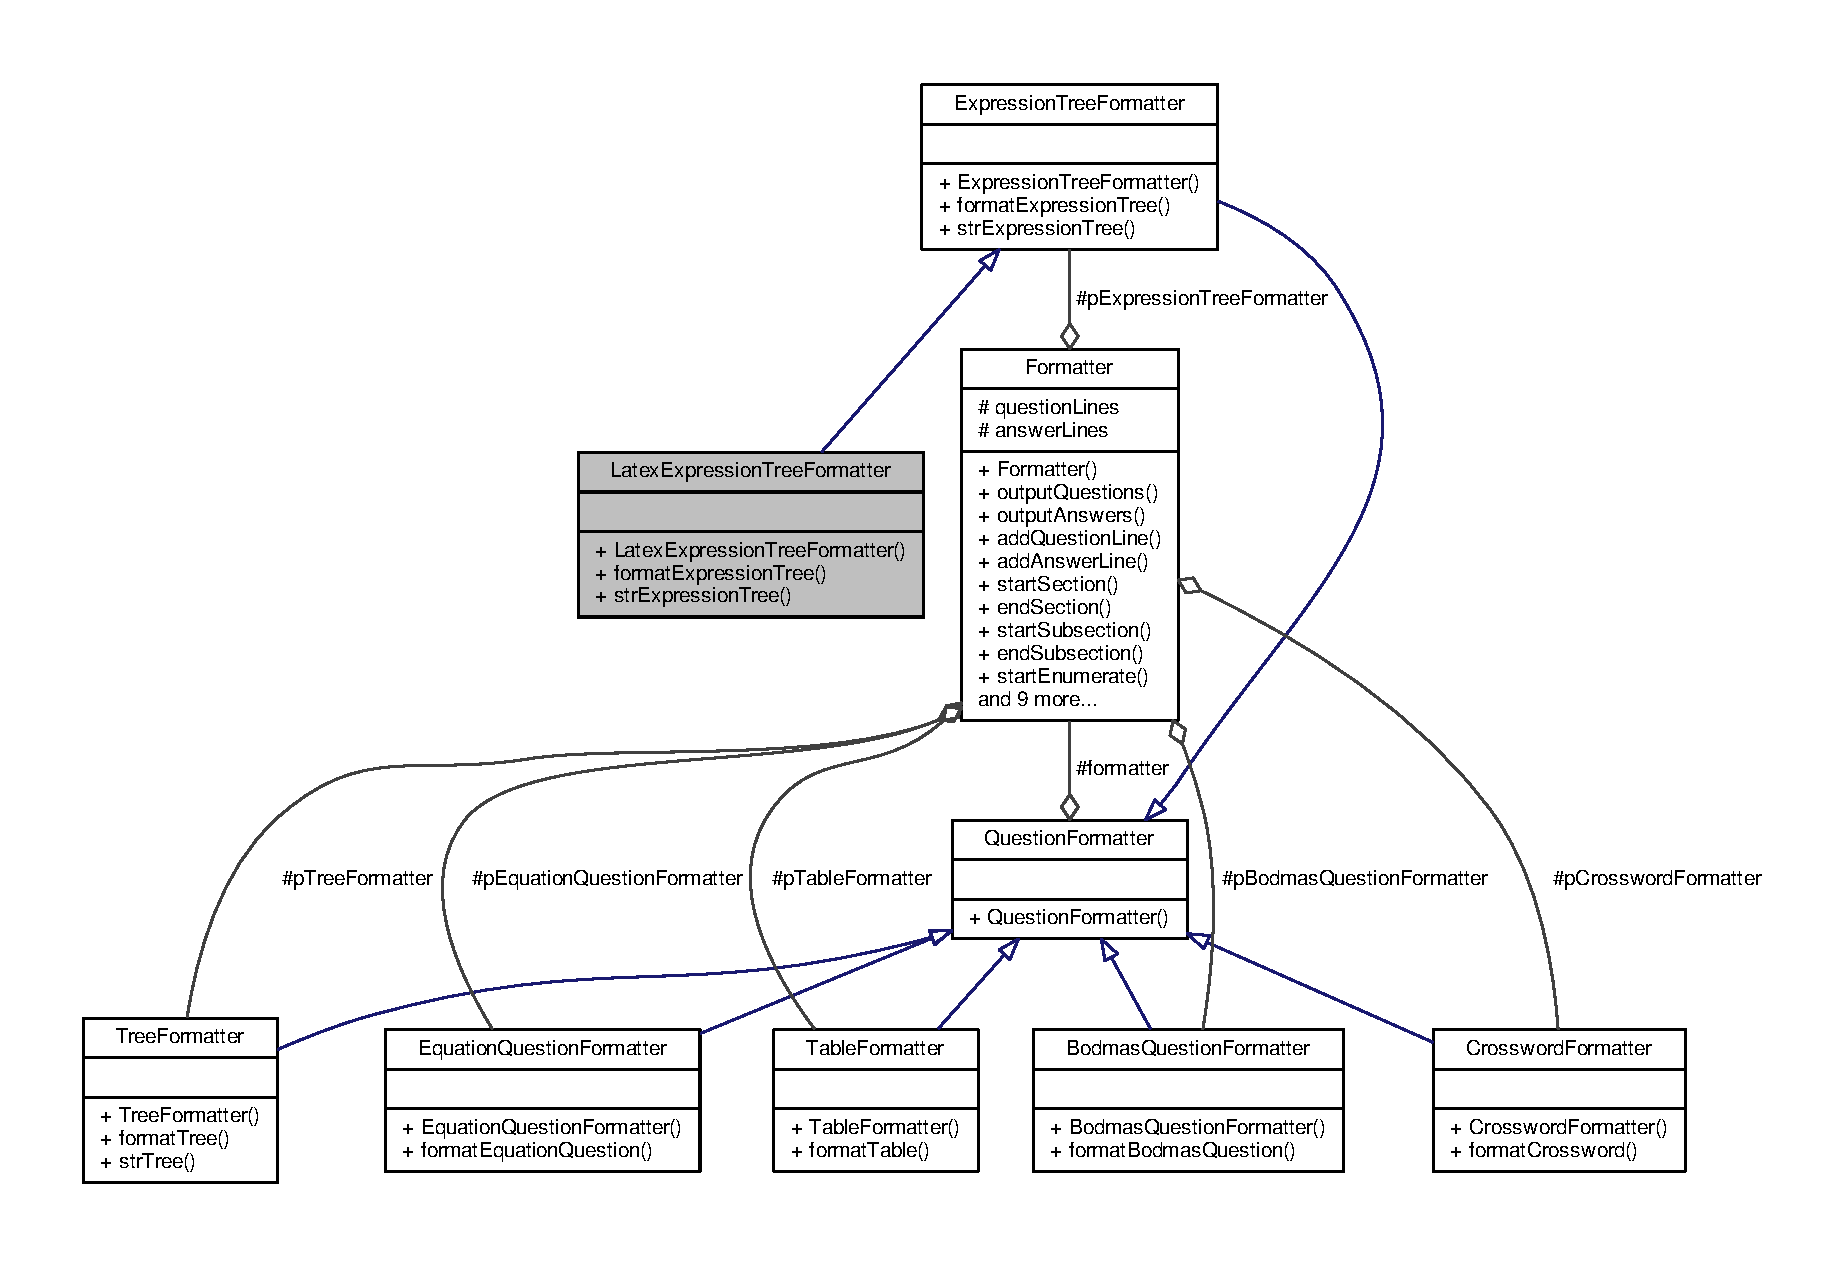
\includegraphics[width=350pt]{classLatexExpressionTreeFormatter__coll__graph}
\end{center}
\end{figure}
\subsection*{Public Member Functions}
\begin{DoxyCompactItemize}
\item 
{\bfseries Latex\+Expression\+Tree\+Formatter} (\hyperlink{classFormatter}{Formatter} $\ast$formatter)\hypertarget{classLatexExpressionTreeFormatter_a549a011e2c44606febeefe6f180ba49d}{}\label{classLatexExpressionTreeFormatter_a549a011e2c44606febeefe6f180ba49d}

\item 
virtual void {\bfseries format\+Expression\+Tree} (\hyperlink{classExpressionTree}{Expression\+Tree} $\ast$tree)\hypertarget{classLatexExpressionTreeFormatter_a124d90415c9f34aaf6f9960c199481ec}{}\label{classLatexExpressionTreeFormatter_a124d90415c9f34aaf6f9960c199481ec}

\item 
std\+::string {\bfseries str\+Expression\+Tree} (\hyperlink{classExpressionTree}{Expression\+Tree} $\ast$tree)\hypertarget{classLatexExpressionTreeFormatter_a1f51232d495926c065c0ace87dadad5b}{}\label{classLatexExpressionTreeFormatter_a1f51232d495926c065c0ace87dadad5b}

\end{DoxyCompactItemize}
\subsection*{Additional Inherited Members}


The documentation for this class was generated from the following files\+:\begin{DoxyCompactItemize}
\item 
/home/douglas/generator2/latexexpressiontreeformatter.\+h\item 
/home/douglas/generator2/latexexpressiontreeformatter.\+cpp\end{DoxyCompactItemize}

\hypertarget{classLatexFormatter}{}\section{Latex\+Formatter Class Reference}
\label{classLatexFormatter}\index{Latex\+Formatter@{Latex\+Formatter}}


Inheritance diagram for Latex\+Formatter\+:
\nopagebreak
\begin{figure}[H]
\begin{center}
\leavevmode
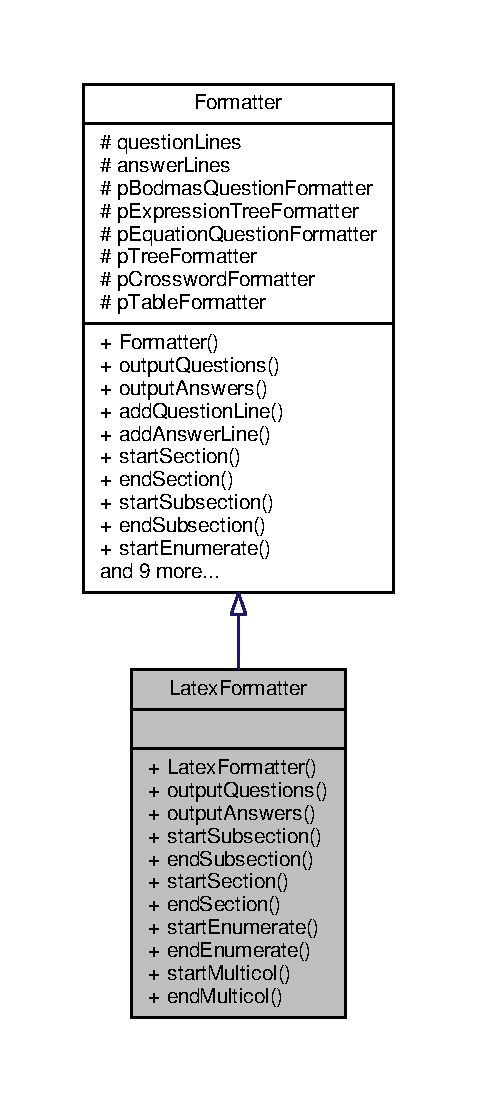
\includegraphics[width=229pt]{classLatexFormatter__inherit__graph}
\end{center}
\end{figure}


Collaboration diagram for Latex\+Formatter\+:
\nopagebreak
\begin{figure}[H]
\begin{center}
\leavevmode
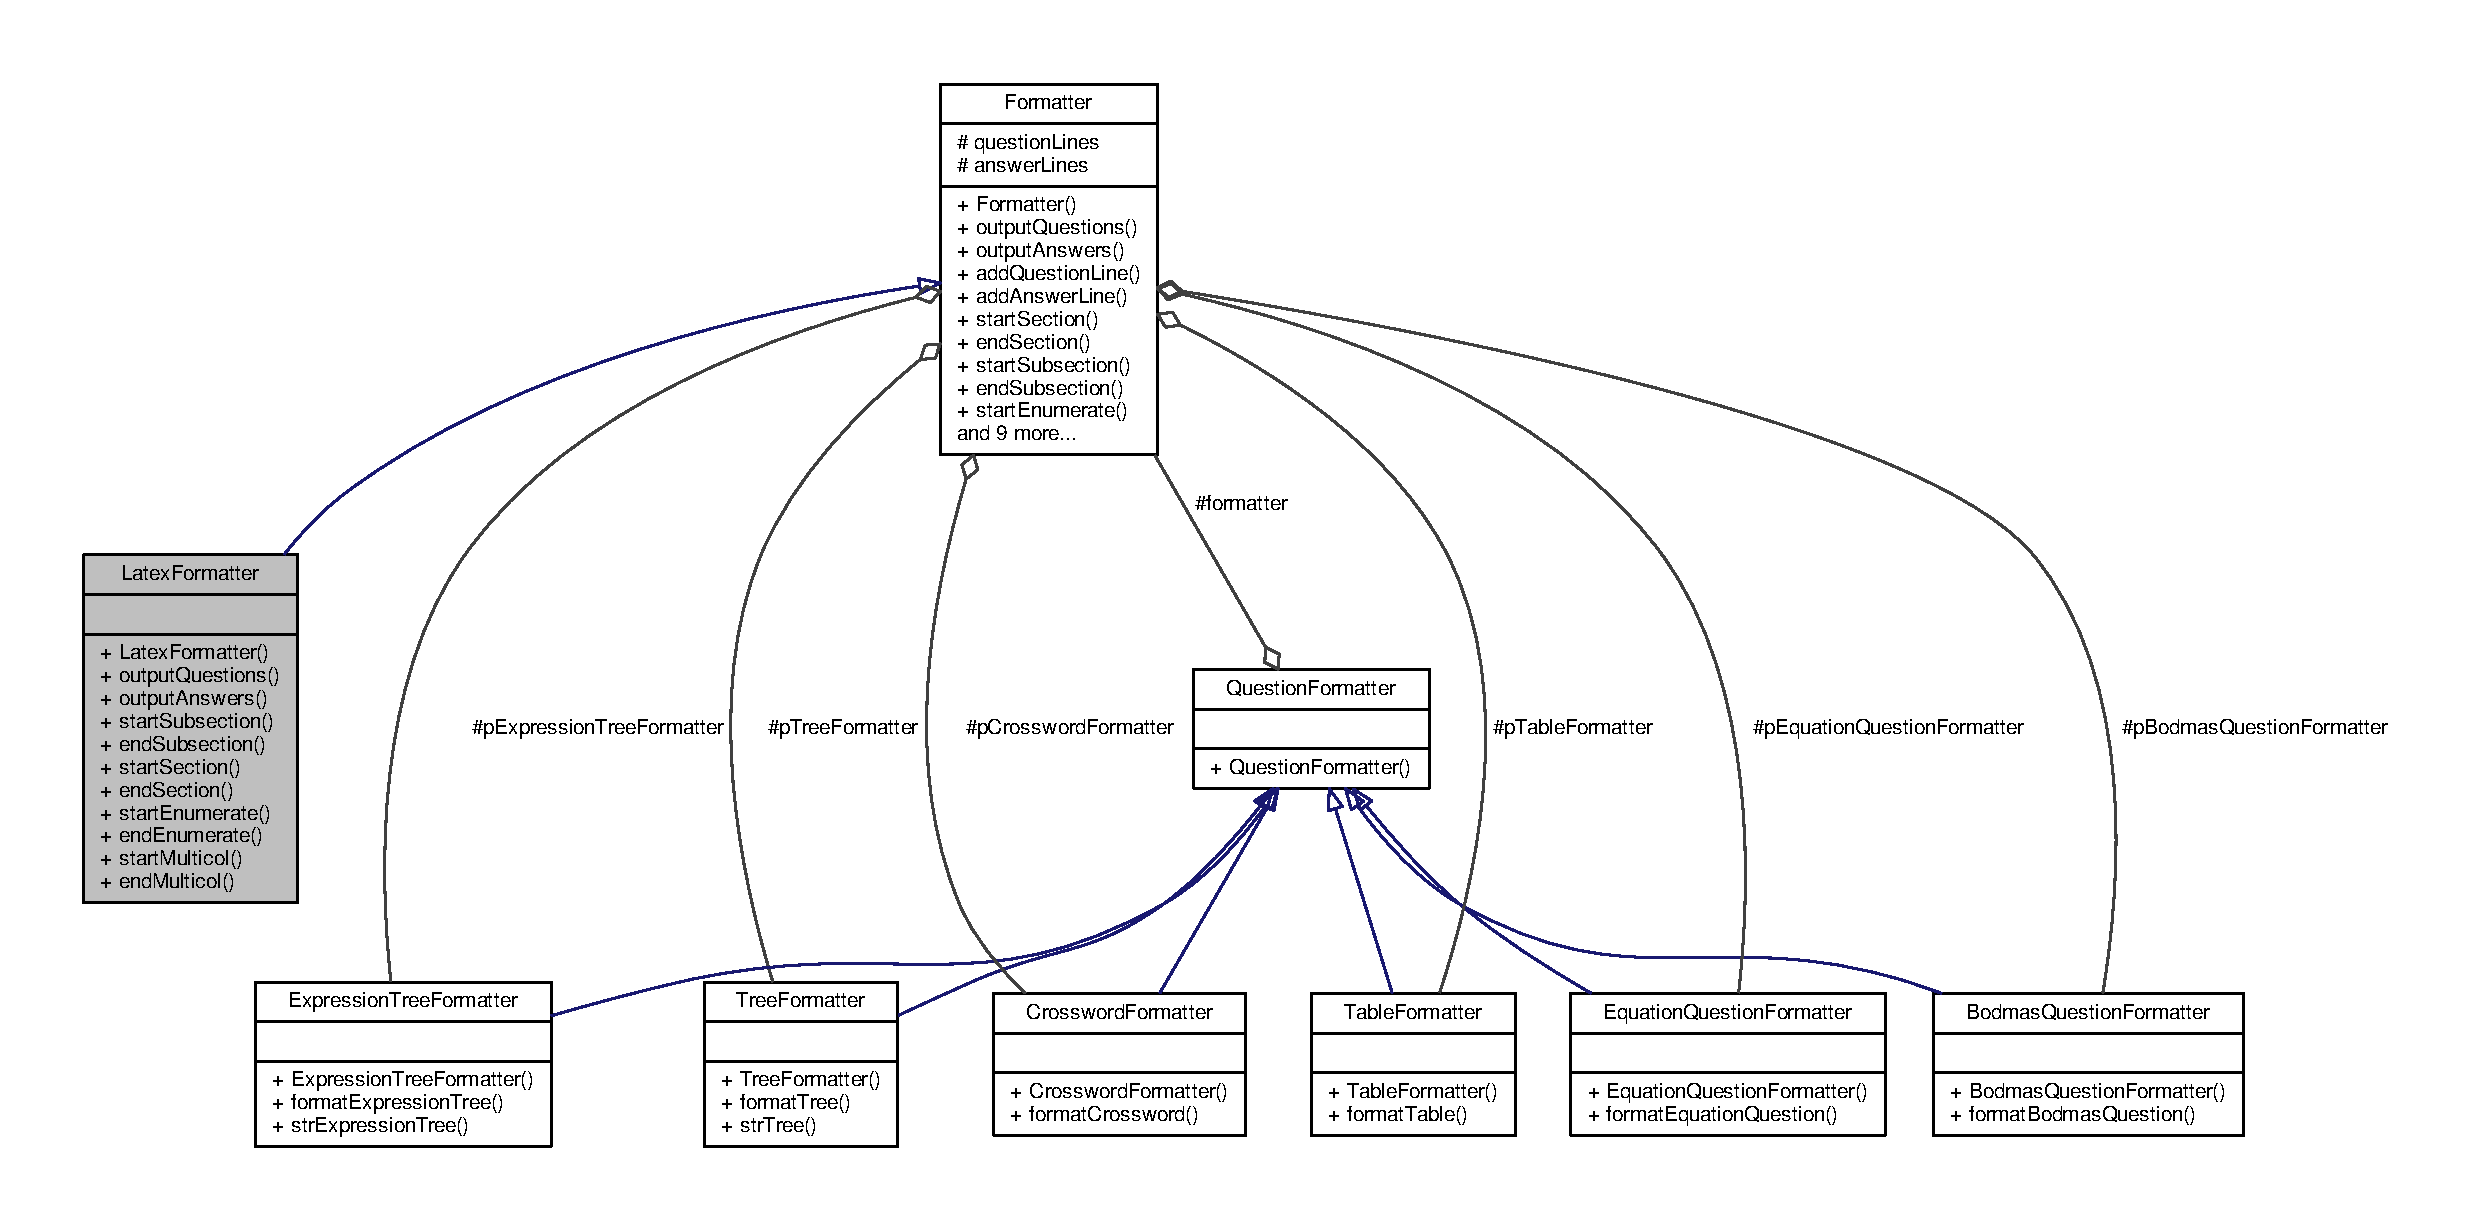
\includegraphics[width=350pt]{classLatexFormatter__coll__graph}
\end{center}
\end{figure}
\subsection*{Public Member Functions}
\begin{DoxyCompactItemize}
\item 
virtual void {\bfseries output\+Questions} (std\+::ostream \&stream)\hypertarget{classLatexFormatter_a23b1afa4afa66cce9da3b5f6fa710aba}{}\label{classLatexFormatter_a23b1afa4afa66cce9da3b5f6fa710aba}

\item 
virtual void {\bfseries output\+Answers} (std\+::ostream \&stream)\hypertarget{classLatexFormatter_ab51c89a5df17ce203bb941b1ce9c8e13}{}\label{classLatexFormatter_ab51c89a5df17ce203bb941b1ce9c8e13}

\item 
virtual void {\bfseries start\+Subsection} (const std\+::string name)\hypertarget{classLatexFormatter_a22c697e684abe2e905ab56fd24b937ca}{}\label{classLatexFormatter_a22c697e684abe2e905ab56fd24b937ca}

\item 
virtual void {\bfseries end\+Subsection} ()\hypertarget{classLatexFormatter_ad5b3f325dad0606582d0b035bb183a7b}{}\label{classLatexFormatter_ad5b3f325dad0606582d0b035bb183a7b}

\item 
virtual void {\bfseries start\+Section} (const std\+::string name)\hypertarget{classLatexFormatter_ac6f15873968fb1eebd6174b3ced286dc}{}\label{classLatexFormatter_ac6f15873968fb1eebd6174b3ced286dc}

\item 
virtual void {\bfseries end\+Section} ()\hypertarget{classLatexFormatter_a029082cd3679671d4e495729b1d61937}{}\label{classLatexFormatter_a029082cd3679671d4e495729b1d61937}

\item 
virtual void {\bfseries start\+Enumerate} ()\hypertarget{classLatexFormatter_a6022104c77fa63e6f2e24358332680d6}{}\label{classLatexFormatter_a6022104c77fa63e6f2e24358332680d6}

\item 
virtual void {\bfseries end\+Enumerate} ()\hypertarget{classLatexFormatter_a748169a459f18cad265869eb78695573}{}\label{classLatexFormatter_a748169a459f18cad265869eb78695573}

\item 
virtual void {\bfseries start\+Multicol} (int num\+Columns)\hypertarget{classLatexFormatter_a116a899aed65c94e4c947ae4a84f7f17}{}\label{classLatexFormatter_a116a899aed65c94e4c947ae4a84f7f17}

\item 
virtual void {\bfseries end\+Multicol} ()\hypertarget{classLatexFormatter_abbb50fd475c80e682baf0364e28ae82b}{}\label{classLatexFormatter_abbb50fd475c80e682baf0364e28ae82b}

\end{DoxyCompactItemize}
\subsection*{Additional Inherited Members}


The documentation for this class was generated from the following files\+:\begin{DoxyCompactItemize}
\item 
/home/douglas/generator2/latexformatter.\+h\item 
/home/douglas/generator2/latexformatter.\+cpp\end{DoxyCompactItemize}

\hypertarget{classLatexTableFormatter}{}\section{Latex\+Table\+Formatter Class Reference}
\label{classLatexTableFormatter}\index{Latex\+Table\+Formatter@{Latex\+Table\+Formatter}}


Inheritance diagram for Latex\+Table\+Formatter\+:
\nopagebreak
\begin{figure}[H]
\begin{center}
\leavevmode
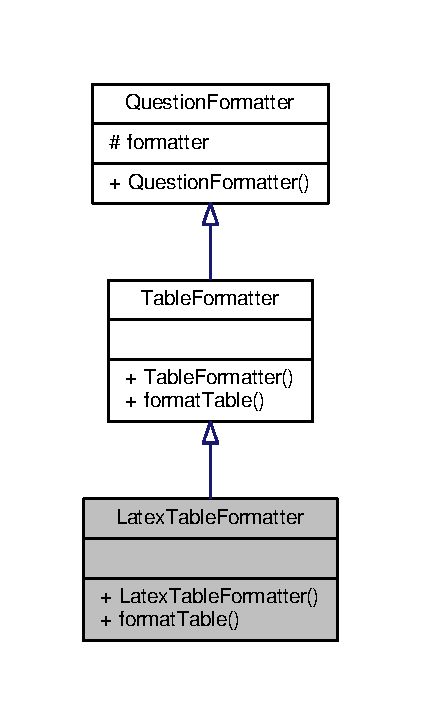
\includegraphics[width=202pt]{classLatexTableFormatter__inherit__graph}
\end{center}
\end{figure}


Collaboration diagram for Latex\+Table\+Formatter\+:
\nopagebreak
\begin{figure}[H]
\begin{center}
\leavevmode
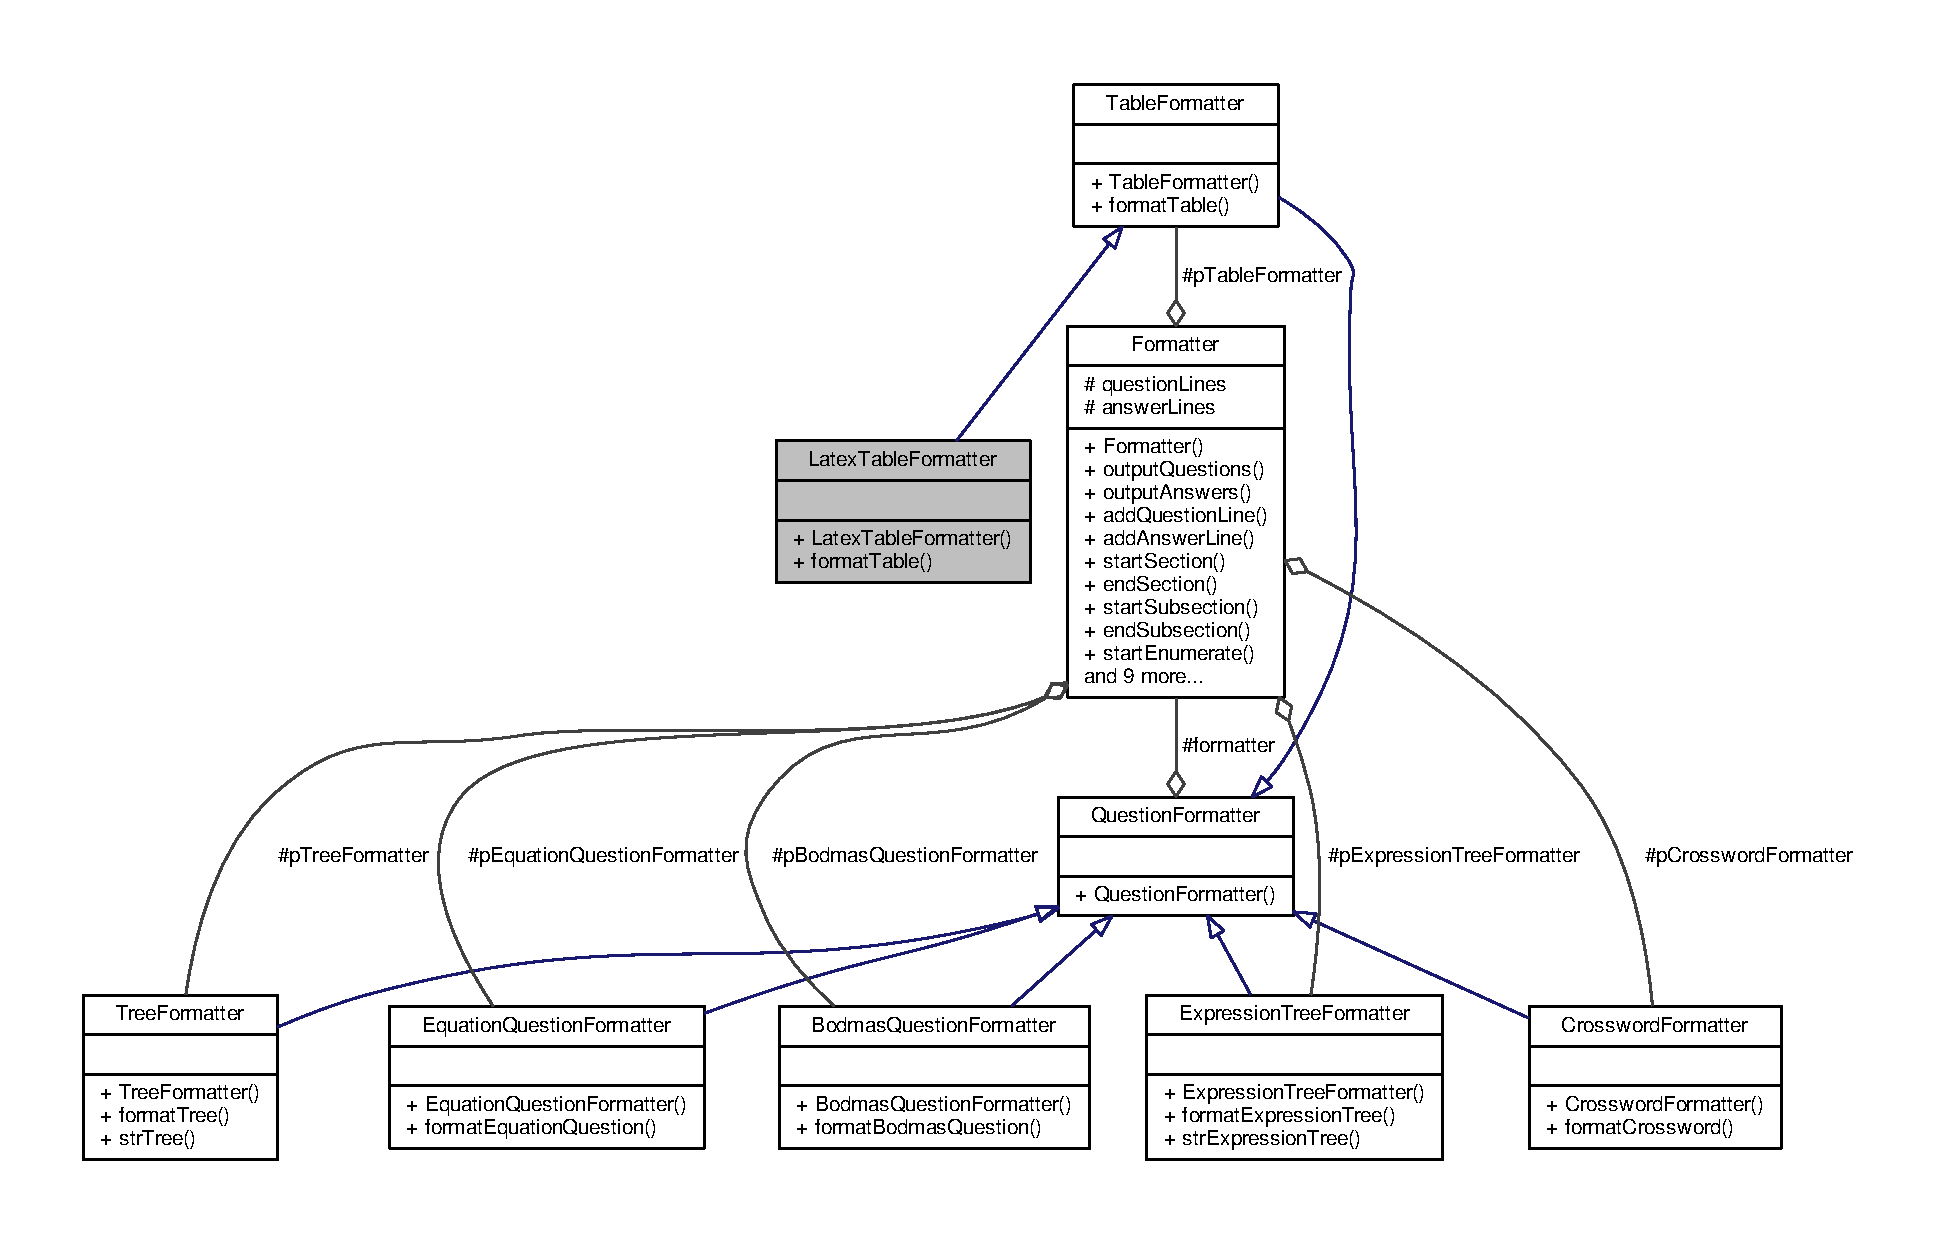
\includegraphics[width=350pt]{classLatexTableFormatter__coll__graph}
\end{center}
\end{figure}
\subsection*{Public Member Functions}
\begin{DoxyCompactItemize}
\item 
{\bfseries Latex\+Table\+Formatter} (\hyperlink{classFormatter}{Formatter} $\ast$formatter)\hypertarget{classLatexTableFormatter_a18735d8bf6647149ac69f923129d70a7}{}\label{classLatexTableFormatter_a18735d8bf6647149ac69f923129d70a7}

\item 
virtual void {\bfseries format\+Table} (\hyperlink{classTable}{Table} $\ast$table)\hypertarget{classLatexTableFormatter_ad2bd549da8ca3463ef668cf7b92a2b3d}{}\label{classLatexTableFormatter_ad2bd549da8ca3463ef668cf7b92a2b3d}

\end{DoxyCompactItemize}
\subsection*{Additional Inherited Members}


The documentation for this class was generated from the following files\+:\begin{DoxyCompactItemize}
\item 
/home/douglas/generator2/latextableformatter.\+h\item 
/home/douglas/generator2/latextableformatter.\+cpp\end{DoxyCompactItemize}

\hypertarget{classLatexTreeFormatter}{}\section{Latex\+Tree\+Formatter Class Reference}
\label{classLatexTreeFormatter}\index{Latex\+Tree\+Formatter@{Latex\+Tree\+Formatter}}


Inheritance diagram for Latex\+Tree\+Formatter\+:
\nopagebreak
\begin{figure}[H]
\begin{center}
\leavevmode
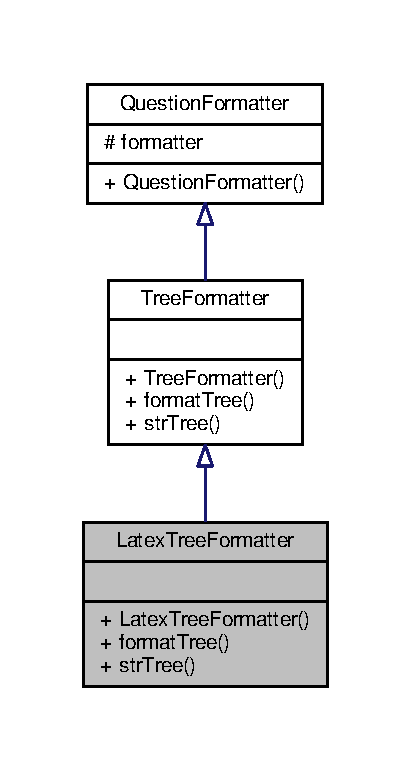
\includegraphics[width=197pt]{classLatexTreeFormatter__inherit__graph}
\end{center}
\end{figure}


Collaboration diagram for Latex\+Tree\+Formatter\+:
\nopagebreak
\begin{figure}[H]
\begin{center}
\leavevmode
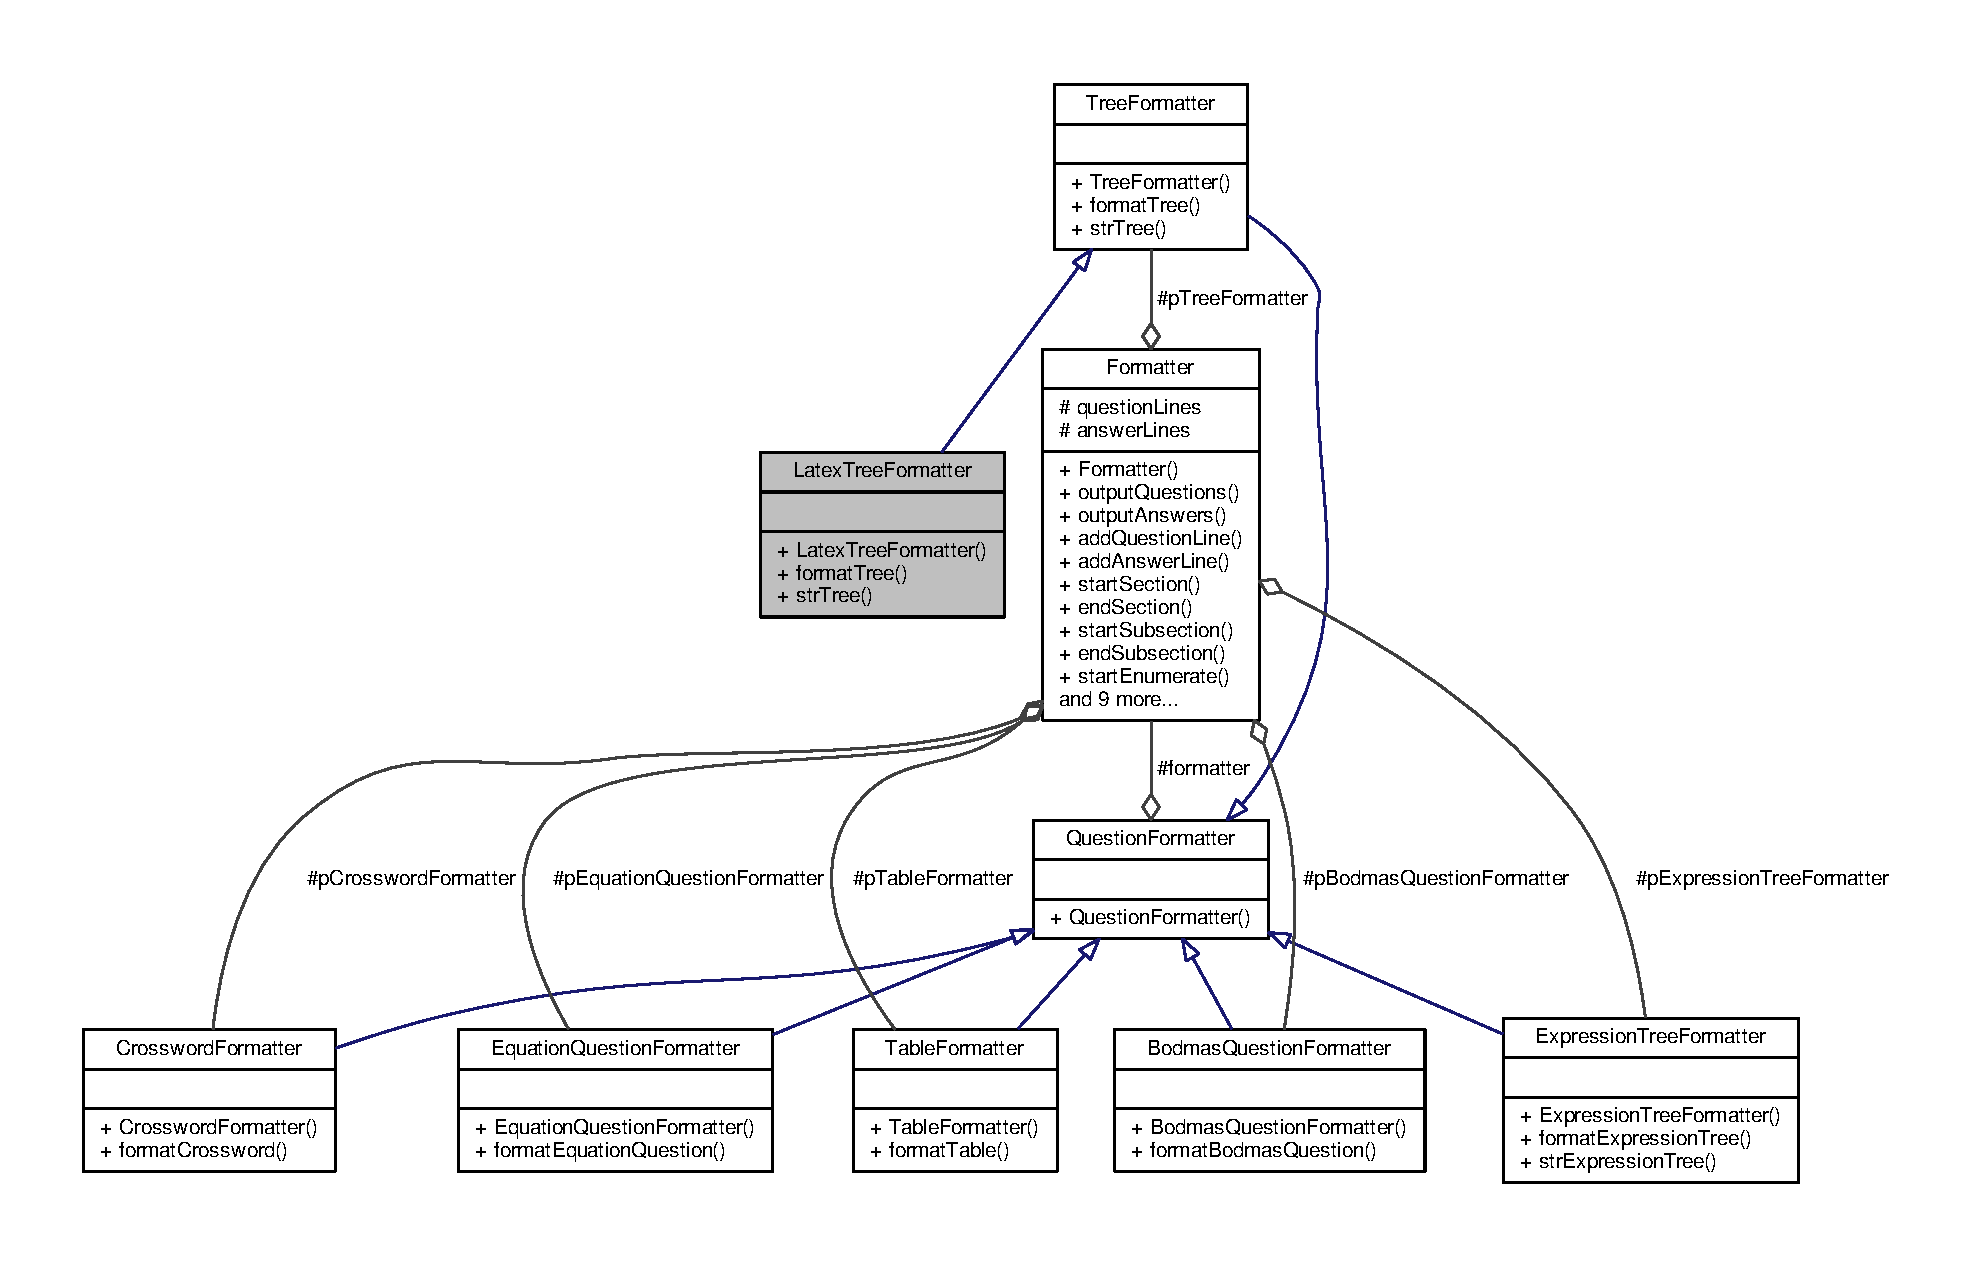
\includegraphics[width=350pt]{classLatexTreeFormatter__coll__graph}
\end{center}
\end{figure}
\subsection*{Public Member Functions}
\begin{DoxyCompactItemize}
\item 
{\bfseries Latex\+Tree\+Formatter} (\hyperlink{classFormatter}{Formatter} $\ast$formatter)\hypertarget{classLatexTreeFormatter_aa294bd613ea6eeb42a75a52f940845a0}{}\label{classLatexTreeFormatter_aa294bd613ea6eeb42a75a52f940845a0}

\item 
virtual void {\bfseries format\+Tree} (\hyperlink{classTree}{Tree} $\ast$tree)\hypertarget{classLatexTreeFormatter_a603cfc39967f65d5f7a54f324266d7e4}{}\label{classLatexTreeFormatter_a603cfc39967f65d5f7a54f324266d7e4}

\item 
virtual std\+::string {\bfseries str\+Tree} (\hyperlink{classTree}{Tree} $\ast$tree)\hypertarget{classLatexTreeFormatter_a4109b73d13c361da7d69668f7a83560b}{}\label{classLatexTreeFormatter_a4109b73d13c361da7d69668f7a83560b}

\end{DoxyCompactItemize}
\subsection*{Additional Inherited Members}


The documentation for this class was generated from the following files\+:\begin{DoxyCompactItemize}
\item 
/home/douglas/generator2/latextreeformatter.\+h\item 
/home/douglas/generator2/latextreeformatter.\+cpp\end{DoxyCompactItemize}

\hypertarget{classMenu}{}\section{Menu Class Reference}
\label{classMenu}\index{Menu@{Menu}}


Collaboration diagram for Menu\+:
\nopagebreak
\begin{figure}[H]
\begin{center}
\leavevmode
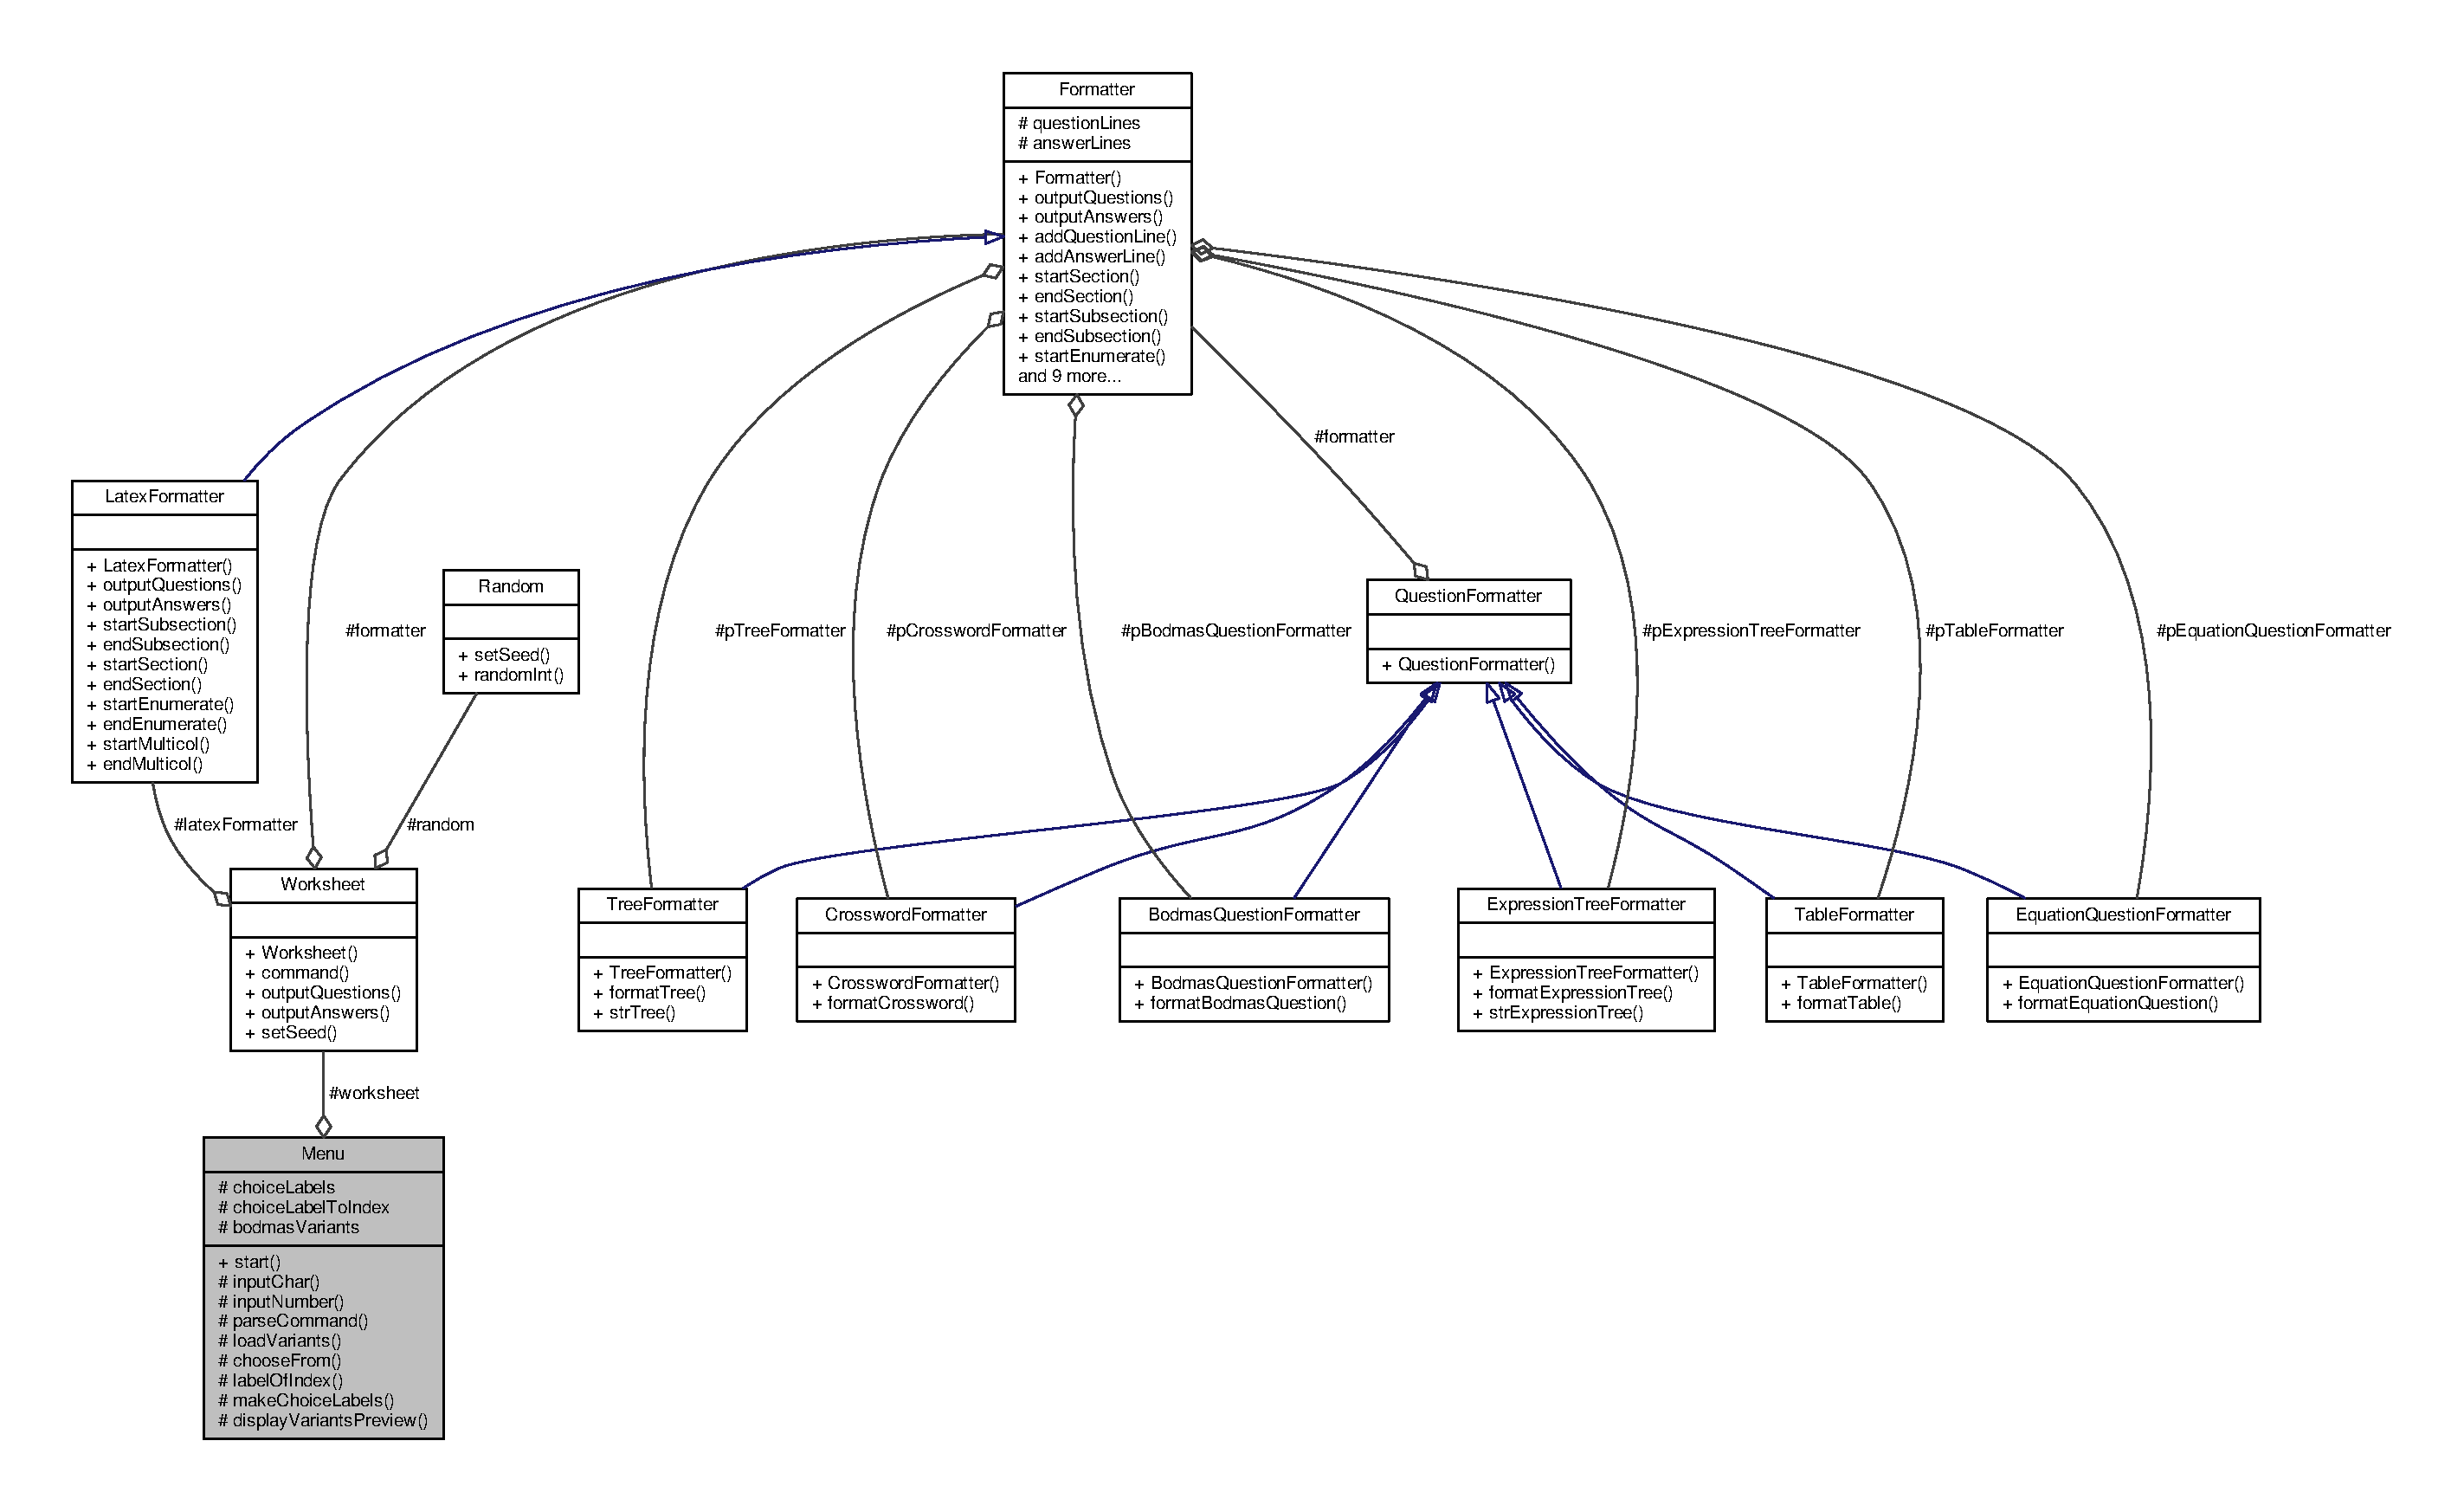
\includegraphics[width=350pt]{classMenu__coll__graph}
\end{center}
\end{figure}
\subsection*{Public Member Functions}
\begin{DoxyCompactItemize}
\item 
void {\bfseries start} ()\hypertarget{classMenu_ae1ec62e738dda7faaaec850bd0b58ffe}{}\label{classMenu_ae1ec62e738dda7faaaec850bd0b58ffe}

\end{DoxyCompactItemize}
\subsection*{Protected Member Functions}
\begin{DoxyCompactItemize}
\item 
char {\bfseries input\+Char} ()\hypertarget{classMenu_a63f7d79414924fa83dceeb160cb3f615}{}\label{classMenu_a63f7d79414924fa83dceeb160cb3f615}

\item 
int {\bfseries input\+Number} ()\hypertarget{classMenu_a8cf9c74ebfcca2a689f9930b238d8633}{}\label{classMenu_a8cf9c74ebfcca2a689f9930b238d8633}

\item 
void {\bfseries parse\+Command} (const std\+::string \&command, std\+::vector$<$ std\+::string $>$ \&args)\hypertarget{classMenu_a4a68d5462687cb599e35b63ae38e7b88}{}\label{classMenu_a4a68d5462687cb599e35b63ae38e7b88}

\item 
void {\bfseries load\+Variants} ()\hypertarget{classMenu_a31523662e2b9d252716aa92cd0de4fa8}{}\label{classMenu_a31523662e2b9d252716aa92cd0de4fa8}

\item 
std\+::string \& {\bfseries choose\+From} (std\+::vector$<$ std\+::string $>$ \&choices)\hypertarget{classMenu_ac3405aa5b352ac8703b9ffa96c491863}{}\label{classMenu_ac3405aa5b352ac8703b9ffa96c491863}

\item 
char {\bfseries label\+Of\+Index} (int index)\hypertarget{classMenu_aef05b36518c368c8cc09fe8b7f936d45}{}\label{classMenu_aef05b36518c368c8cc09fe8b7f936d45}

\item 
void {\bfseries make\+Choice\+Labels} ()\hypertarget{classMenu_a48c9d012d1929fd523231a2fcba114a9}{}\label{classMenu_a48c9d012d1929fd523231a2fcba114a9}

\item 
void {\bfseries display\+Variants\+Preview} (std\+::vector$<$ std\+::string $>$ \&variants)\hypertarget{classMenu_aef06601147fe4e258b855b3e9df9e165}{}\label{classMenu_aef06601147fe4e258b855b3e9df9e165}

\end{DoxyCompactItemize}
\subsection*{Protected Attributes}
\begin{DoxyCompactItemize}
\item 
std\+::string {\bfseries choice\+Labels}\hypertarget{classMenu_a672f60ceacb5575bae40420833c6ec5c}{}\label{classMenu_a672f60ceacb5575bae40420833c6ec5c}

\item 
std\+::map$<$ char, int $>$ {\bfseries choice\+Label\+To\+Index}\hypertarget{classMenu_af532dd3049db66e1685446259f23a9d8}{}\label{classMenu_af532dd3049db66e1685446259f23a9d8}

\item 
std\+::vector$<$ std\+::string $>$ {\bfseries bodmas\+Variants}\hypertarget{classMenu_ac57df072a5c984cc013f96e6dc7e37f7}{}\label{classMenu_ac57df072a5c984cc013f96e6dc7e37f7}

\item 
\hyperlink{classWorksheet}{Worksheet} {\bfseries worksheet}\hypertarget{classMenu_a34d304dccfe737f272d9f1c7be00bda0}{}\label{classMenu_a34d304dccfe737f272d9f1c7be00bda0}

\end{DoxyCompactItemize}


The documentation for this class was generated from the following files\+:\begin{DoxyCompactItemize}
\item 
/home/douglas/generator2/menu.\+h\item 
/home/douglas/generator2/menu.\+cpp\end{DoxyCompactItemize}

\hypertarget{classNode}{}\section{Node Class Reference}
\label{classNode}\index{Node@{Node}}


Collaboration diagram for Node\+:
\nopagebreak
\begin{figure}[H]
\begin{center}
\leavevmode
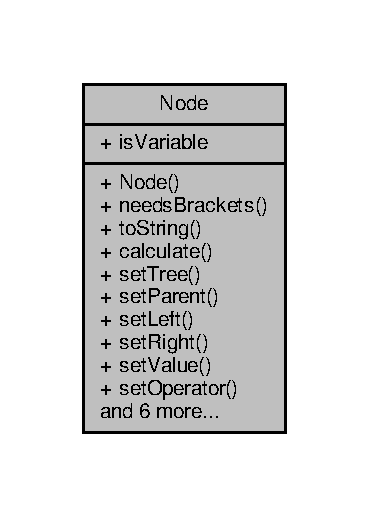
\includegraphics[width=177pt]{classNode__coll__graph}
\end{center}
\end{figure}
\subsection*{Public Member Functions}
\begin{DoxyCompactItemize}
\item 
bool {\bfseries needs\+Brackets} ()\hypertarget{classNode_a261c181a5903859426230097c9733441}{}\label{classNode_a261c181a5903859426230097c9733441}

\item 
std\+::string {\bfseries to\+String} ()\hypertarget{classNode_ab68ba2e4b8b4b4aa5cd9cdcfe03277f3}{}\label{classNode_ab68ba2e4b8b4b4aa5cd9cdcfe03277f3}

\item 
void {\bfseries calculate} ()\hypertarget{classNode_afef1e95a8f3a2056feec47a44ce0007c}{}\label{classNode_afef1e95a8f3a2056feec47a44ce0007c}

\item 
void {\bfseries set\+Tree} (\hyperlink{classTree}{Tree} $\ast$tree)\hypertarget{classNode_aafb43f6bd3ce1e8d0a6e339ce33afec7}{}\label{classNode_aafb43f6bd3ce1e8d0a6e339ce33afec7}

\item 
void {\bfseries set\+Parent} (\hyperlink{classNode}{Node} $\ast$parent)\hypertarget{classNode_ab5f0786bcb59591c528efb0b776797fc}{}\label{classNode_ab5f0786bcb59591c528efb0b776797fc}

\item 
void {\bfseries set\+Left} (\hyperlink{classNode}{Node} $\ast$left)\hypertarget{classNode_a9022102d755b999dc0f6ed97142b80f2}{}\label{classNode_a9022102d755b999dc0f6ed97142b80f2}

\item 
void {\bfseries set\+Right} (\hyperlink{classNode}{Node} $\ast$right)\hypertarget{classNode_ab93f8f7d56241bc2b978595b208604dc}{}\label{classNode_ab93f8f7d56241bc2b978595b208604dc}

\item 
void {\bfseries set\+Value} (int value)\hypertarget{classNode_a9e337c1790152faf945a87207d7e1125}{}\label{classNode_a9e337c1790152faf945a87207d7e1125}

\item 
void {\bfseries set\+Operator} (int op)\hypertarget{classNode_a9e474c9df32b49bd241b0057c35cd91d}{}\label{classNode_a9e474c9df32b49bd241b0057c35cd91d}

\item 
\hyperlink{classTree}{Tree} $\ast$ {\bfseries get\+Tree} ()\hypertarget{classNode_ab1ca8e497b3c925507a36b4988cd6161}{}\label{classNode_ab1ca8e497b3c925507a36b4988cd6161}

\item 
\hyperlink{classNode}{Node} $\ast$ {\bfseries get\+Parent} ()\hypertarget{classNode_a220a8d64cb0df1cce083ed38c1260615}{}\label{classNode_a220a8d64cb0df1cce083ed38c1260615}

\item 
\hyperlink{classNode}{Node} $\ast$ {\bfseries get\+Left} ()\hypertarget{classNode_ac73b72f9a1fbdb23cc5c031afaccb415}{}\label{classNode_ac73b72f9a1fbdb23cc5c031afaccb415}

\item 
\hyperlink{classNode}{Node} $\ast$ {\bfseries get\+Right} ()\hypertarget{classNode_a47f547ea1e8703057e6d345f238104d1}{}\label{classNode_a47f547ea1e8703057e6d345f238104d1}

\item 
int {\bfseries get\+Value} ()\hypertarget{classNode_affbe7f986fd7ed645c5bc361363e96ec}{}\label{classNode_affbe7f986fd7ed645c5bc361363e96ec}

\item 
int {\bfseries get\+Operator} ()\hypertarget{classNode_a705ad4b608cfd4d03d0127021979517b}{}\label{classNode_a705ad4b608cfd4d03d0127021979517b}

\end{DoxyCompactItemize}
\subsection*{Public Attributes}
\begin{DoxyCompactItemize}
\item 
bool {\bfseries is\+Variable}\hypertarget{classNode_a2ef8b6435d78a530427cb1b19e72971f}{}\label{classNode_a2ef8b6435d78a530427cb1b19e72971f}

\end{DoxyCompactItemize}


The documentation for this class was generated from the following files\+:\begin{DoxyCompactItemize}
\item 
/home/douglas/generator2/node.\+h\item 
/home/douglas/generator2/node.\+cpp\end{DoxyCompactItemize}

\hypertarget{classQuestion}{}\section{Question Class Reference}
\label{classQuestion}\index{Question@{Question}}


Inheritance diagram for Question\+:
\nopagebreak
\begin{figure}[H]
\begin{center}
\leavevmode
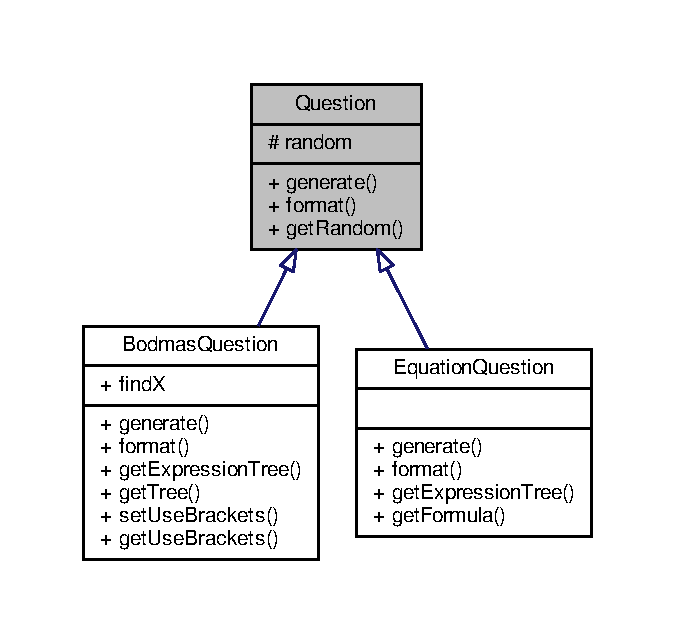
\includegraphics[width=324pt]{classQuestion__inherit__graph}
\end{center}
\end{figure}


Collaboration diagram for Question\+:
\nopagebreak
\begin{figure}[H]
\begin{center}
\leavevmode
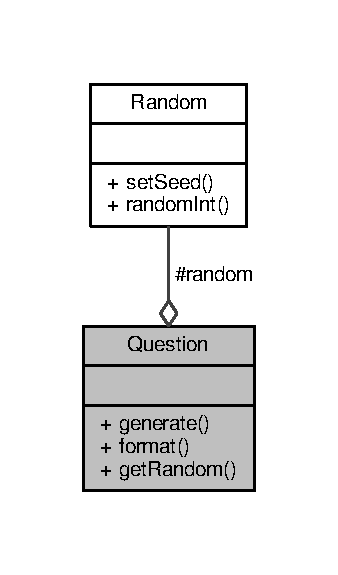
\includegraphics[width=162pt]{classQuestion__coll__graph}
\end{center}
\end{figure}
\subsection*{Public Member Functions}
\begin{DoxyCompactItemize}
\item 
virtual void {\bfseries generate} (std\+::vector$<$ std\+::string $>$ \&args)=0\hypertarget{classQuestion_a8d918509068d607a936cdd1e697a210a}{}\label{classQuestion_a8d918509068d607a936cdd1e697a210a}

\item 
virtual void {\bfseries format} (\hyperlink{classFormatter}{Formatter} $\ast$formatter)=0\hypertarget{classQuestion_a6e71cfa6da8779cf2f7e294c6250647e}{}\label{classQuestion_a6e71cfa6da8779cf2f7e294c6250647e}

\item 
\hyperlink{classRandom}{Random} \& {\bfseries get\+Random} ()\hypertarget{classQuestion_a445fff50c6662c095b0bf2585c3d14fe}{}\label{classQuestion_a445fff50c6662c095b0bf2585c3d14fe}

\end{DoxyCompactItemize}
\subsection*{Protected Attributes}
\begin{DoxyCompactItemize}
\item 
\hyperlink{classRandom}{Random} {\bfseries random}\hypertarget{classQuestion_ab5cc8c4214739c66c418155c338bfeac}{}\label{classQuestion_ab5cc8c4214739c66c418155c338bfeac}

\end{DoxyCompactItemize}


The documentation for this class was generated from the following files\+:\begin{DoxyCompactItemize}
\item 
/home/douglas/generator2/question.\+h\item 
/home/douglas/generator2/question.\+cpp\end{DoxyCompactItemize}

\hypertarget{classQuestionFormatter}{}\section{Question\+Formatter Class Reference}
\label{classQuestionFormatter}\index{Question\+Formatter@{Question\+Formatter}}


Inheritance diagram for Question\+Formatter\+:
\nopagebreak
\begin{figure}[H]
\begin{center}
\leavevmode
\includegraphics[width=350pt]{classQuestionFormatter__inherit__graph}
\end{center}
\end{figure}


Collaboration diagram for Question\+Formatter\+:
\nopagebreak
\begin{figure}[H]
\begin{center}
\leavevmode
\includegraphics[width=350pt]{classQuestionFormatter__coll__graph}
\end{center}
\end{figure}
\subsection*{Public Member Functions}
\begin{DoxyCompactItemize}
\item 
{\bfseries Question\+Formatter} (\hyperlink{classFormatter}{Formatter} $\ast$formatter)\hypertarget{classQuestionFormatter_acfe7d87dff4ef32b73d2b6145a174dd9}{}\label{classQuestionFormatter_acfe7d87dff4ef32b73d2b6145a174dd9}

\end{DoxyCompactItemize}
\subsection*{Protected Attributes}
\begin{DoxyCompactItemize}
\item 
\hyperlink{classFormatter}{Formatter} $\ast$ {\bfseries formatter}\hypertarget{classQuestionFormatter_a87b39e5c6907234f40e418bee3031051}{}\label{classQuestionFormatter_a87b39e5c6907234f40e418bee3031051}

\end{DoxyCompactItemize}


The documentation for this class was generated from the following files\+:\begin{DoxyCompactItemize}
\item 
/home/douglas/generator2/questionformatter.\+h\item 
/home/douglas/generator2/questionformatter.\+cpp\end{DoxyCompactItemize}

\hypertarget{classRandom}{}\section{Random Class Reference}
\label{classRandom}\index{Random@{Random}}


Collaboration diagram for Random\+:
\nopagebreak
\begin{figure}[H]
\begin{center}
\leavevmode
\includegraphics[width=155pt]{classRandom__coll__graph}
\end{center}
\end{figure}
\subsection*{Public Member Functions}
\begin{DoxyCompactItemize}
\item 
void {\bfseries set\+Seed} (int seed)\hypertarget{classRandom_a84f6d30f1cf64ef0cfe6d4ddd60269e9}{}\label{classRandom_a84f6d30f1cf64ef0cfe6d4ddd60269e9}

\item 
int {\bfseries random\+Int} (int min, int max)\hypertarget{classRandom_a6a9dfc13b6af6788018738bb132656c7}{}\label{classRandom_a6a9dfc13b6af6788018738bb132656c7}

\end{DoxyCompactItemize}


The documentation for this class was generated from the following files\+:\begin{DoxyCompactItemize}
\item 
/home/douglas/generator2/random.\+h\item 
/home/douglas/generator2/random.\+cpp\end{DoxyCompactItemize}

\hypertarget{classSwapper}{}\section{Swapper Class Reference}
\label{classSwapper}\index{Swapper@{Swapper}}


Inheritance diagram for Swapper\+:
\nopagebreak
\begin{figure}[H]
\begin{center}
\leavevmode
\includegraphics[width=350pt]{classSwapper__inherit__graph}
\end{center}
\end{figure}


Collaboration diagram for Swapper\+:
\nopagebreak
\begin{figure}[H]
\begin{center}
\leavevmode
\includegraphics[width=161pt]{classSwapper__coll__graph}
\end{center}
\end{figure}
\subsection*{Public Member Functions}
\begin{DoxyCompactItemize}
\item 
virtual bool {\bfseries can\+Swap} (\hyperlink{classNode}{Node} $\ast$node)=0\hypertarget{classSwapper_a3e40c0156db41717004af48a98c97bee}{}\label{classSwapper_a3e40c0156db41717004af48a98c97bee}

\item 
virtual void {\bfseries swap} (\hyperlink{classNode}{Node} $\ast$node)=0\hypertarget{classSwapper_a0c9f16ac8a863050245d3307d4ab3aea}{}\label{classSwapper_a0c9f16ac8a863050245d3307d4ab3aea}

\item 
void {\bfseries set\+Enabled} (bool b)\hypertarget{classSwapper_a11aab095194ce84106c45142e5952c9a}{}\label{classSwapper_a11aab095194ce84106c45142e5952c9a}

\end{DoxyCompactItemize}
\subsection*{Protected Member Functions}
\begin{DoxyCompactItemize}
\item 
void {\bfseries replace} (\hyperlink{classNode}{Node} $\ast$node, \hyperlink{classNode}{Node} $\ast$other)\hypertarget{classSwapper_a8d100df849fafafb520235999c838c02}{}\label{classSwapper_a8d100df849fafafb520235999c838c02}

\end{DoxyCompactItemize}
\subsection*{Protected Attributes}
\begin{DoxyCompactItemize}
\item 
\hyperlink{classRandom}{Random} {\bfseries random}\hypertarget{classSwapper_aaa71eb757ba363865f1d9e39fe9c6732}{}\label{classSwapper_aaa71eb757ba363865f1d9e39fe9c6732}

\item 
bool {\bfseries enabled}\hypertarget{classSwapper_ab13ddb9c1f01cb9cd18d5ecfcac6b37a}{}\label{classSwapper_ab13ddb9c1f01cb9cd18d5ecfcac6b37a}

\end{DoxyCompactItemize}


The documentation for this class was generated from the following files\+:\begin{DoxyCompactItemize}
\item 
/home/douglas/generator2/swapper.\+h\item 
/home/douglas/generator2/swapper.\+cpp\end{DoxyCompactItemize}

\hypertarget{classSwapperDivide}{}\section{Swapper\+Divide Class Reference}
\label{classSwapperDivide}\index{Swapper\+Divide@{Swapper\+Divide}}


Inheritance diagram for Swapper\+Divide\+:
\nopagebreak
\begin{figure}[H]
\begin{center}
\leavevmode
\includegraphics[width=163pt]{classSwapperDivide__inherit__graph}
\end{center}
\end{figure}


Collaboration diagram for Swapper\+Divide\+:
\nopagebreak
\begin{figure}[H]
\begin{center}
\leavevmode
\includegraphics[width=163pt]{classSwapperDivide__coll__graph}
\end{center}
\end{figure}
\subsection*{Public Member Functions}
\begin{DoxyCompactItemize}
\item 
virtual bool {\bfseries can\+Swap} (\hyperlink{classNode}{Node} $\ast$node)\hypertarget{classSwapperDivide_aa50ae3351ddc3917bcbeb1b22728cc63}{}\label{classSwapperDivide_aa50ae3351ddc3917bcbeb1b22728cc63}

\item 
virtual void {\bfseries swap} (\hyperlink{classNode}{Node} $\ast$node)\hypertarget{classSwapperDivide_af0816de678e18182316321fb93c7c033}{}\label{classSwapperDivide_af0816de678e18182316321fb93c7c033}

\end{DoxyCompactItemize}
\subsection*{Additional Inherited Members}


The documentation for this class was generated from the following files\+:\begin{DoxyCompactItemize}
\item 
/home/douglas/generator2/swapperdivide.\+h\item 
/home/douglas/generator2/swapperdivide.\+cpp\end{DoxyCompactItemize}

\hypertarget{classSwapperMinus}{}\section{Swapper\+Minus Class Reference}
\label{classSwapperMinus}\index{Swapper\+Minus@{Swapper\+Minus}}


Inheritance diagram for Swapper\+Minus\+:
\nopagebreak
\begin{figure}[H]
\begin{center}
\leavevmode
\includegraphics[width=161pt]{classSwapperMinus__inherit__graph}
\end{center}
\end{figure}


Collaboration diagram for Swapper\+Minus\+:
\nopagebreak
\begin{figure}[H]
\begin{center}
\leavevmode
\includegraphics[width=162pt]{classSwapperMinus__coll__graph}
\end{center}
\end{figure}
\subsection*{Public Member Functions}
\begin{DoxyCompactItemize}
\item 
virtual bool {\bfseries can\+Swap} (\hyperlink{classNode}{Node} $\ast$node)\hypertarget{classSwapperMinus_a8beb0fa80bd22b934af250d7b073b265}{}\label{classSwapperMinus_a8beb0fa80bd22b934af250d7b073b265}

\item 
virtual void {\bfseries swap} (\hyperlink{classNode}{Node} $\ast$node)\hypertarget{classSwapperMinus_a11efab75180cc3f0195f4f30309219f3}{}\label{classSwapperMinus_a11efab75180cc3f0195f4f30309219f3}

\end{DoxyCompactItemize}
\subsection*{Additional Inherited Members}


The documentation for this class was generated from the following files\+:\begin{DoxyCompactItemize}
\item 
/home/douglas/generator2/swapperminus.\+h\item 
/home/douglas/generator2/swapperminus.\+cpp\end{DoxyCompactItemize}

\hypertarget{classSwapperPlus}{}\section{Swapper\+Plus Class Reference}
\label{classSwapperPlus}\index{Swapper\+Plus@{Swapper\+Plus}}


Inheritance diagram for Swapper\+Plus\+:
\nopagebreak
\begin{figure}[H]
\begin{center}
\leavevmode
\includegraphics[width=160pt]{classSwapperPlus__inherit__graph}
\end{center}
\end{figure}


Collaboration diagram for Swapper\+Plus\+:
\nopagebreak
\begin{figure}[H]
\begin{center}
\leavevmode
\includegraphics[width=161pt]{classSwapperPlus__coll__graph}
\end{center}
\end{figure}
\subsection*{Public Member Functions}
\begin{DoxyCompactItemize}
\item 
virtual bool {\bfseries can\+Swap} (\hyperlink{classNode}{Node} $\ast$node)\hypertarget{classSwapperPlus_a827dd0ad5d25df7c4eca350d9d92fe50}{}\label{classSwapperPlus_a827dd0ad5d25df7c4eca350d9d92fe50}

\item 
virtual void {\bfseries swap} (\hyperlink{classNode}{Node} $\ast$node)\hypertarget{classSwapperPlus_ae5124c7b4793158d2fa5aba1cdf89c54}{}\label{classSwapperPlus_ae5124c7b4793158d2fa5aba1cdf89c54}

\end{DoxyCompactItemize}
\subsection*{Additional Inherited Members}


The documentation for this class was generated from the following files\+:\begin{DoxyCompactItemize}
\item 
/home/douglas/generator2/swapperplus.\+h\item 
/home/douglas/generator2/swapperplus.\+cpp\end{DoxyCompactItemize}

\hypertarget{classSwapperTimes}{}\section{Swapper\+Times Class Reference}
\label{classSwapperTimes}\index{Swapper\+Times@{Swapper\+Times}}


Inheritance diagram for Swapper\+Times\+:
\nopagebreak
\begin{figure}[H]
\begin{center}
\leavevmode
\includegraphics[width=162pt]{classSwapperTimes__inherit__graph}
\end{center}
\end{figure}


Collaboration diagram for Swapper\+Times\+:
\nopagebreak
\begin{figure}[H]
\begin{center}
\leavevmode
\includegraphics[width=162pt]{classSwapperTimes__coll__graph}
\end{center}
\end{figure}
\subsection*{Public Member Functions}
\begin{DoxyCompactItemize}
\item 
virtual bool {\bfseries can\+Swap} (\hyperlink{classNode}{Node} $\ast$node)\hypertarget{classSwapperTimes_a58ef0e5a1df11303f6292ac0a5e5f548}{}\label{classSwapperTimes_a58ef0e5a1df11303f6292ac0a5e5f548}

\item 
virtual void {\bfseries swap} (\hyperlink{classNode}{Node} $\ast$node)\hypertarget{classSwapperTimes_ab9e3aa678acdfccd5e00cd16cc6eec0d}{}\label{classSwapperTimes_ab9e3aa678acdfccd5e00cd16cc6eec0d}

\end{DoxyCompactItemize}
\subsection*{Additional Inherited Members}


The documentation for this class was generated from the following files\+:\begin{DoxyCompactItemize}
\item 
/home/douglas/generator2/swappertimes.\+h\item 
/home/douglas/generator2/swappertimes.\+cpp\end{DoxyCompactItemize}

\hypertarget{classSwappingBuilder}{}\section{Swapping\+Builder Class Reference}
\label{classSwappingBuilder}\index{Swapping\+Builder@{Swapping\+Builder}}


Collaboration diagram for Swapping\+Builder\+:
\nopagebreak
\begin{figure}[H]
\begin{center}
\leavevmode
\includegraphics[width=184pt]{classSwappingBuilder__coll__graph}
\end{center}
\end{figure}
\subsection*{Public Member Functions}
\begin{DoxyCompactItemize}
\item 
void {\bfseries build} (\hyperlink{classTree}{Tree} $\ast$tree)\hypertarget{classSwappingBuilder_a813d17403b7e0d5bc073eafe8827955f}{}\label{classSwappingBuilder_a813d17403b7e0d5bc073eafe8827955f}

\item 
void {\bfseries enable\+Swapper} (std\+::string name)\hypertarget{classSwappingBuilder_a83eec69297b400b6255111c583c47961}{}\label{classSwappingBuilder_a83eec69297b400b6255111c583c47961}

\end{DoxyCompactItemize}


The documentation for this class was generated from the following files\+:\begin{DoxyCompactItemize}
\item 
/home/douglas/generator2/swappingbuilder.\+h\item 
/home/douglas/generator2/swappingbuilder.\+cpp\end{DoxyCompactItemize}

\hypertarget{classTable}{}\section{Table Class Reference}
\label{classTable}\index{Table@{Table}}


Inheritance diagram for Table\+:
\nopagebreak
\begin{figure}[H]
\begin{center}
\leavevmode
\includegraphics[width=180pt]{classTable__inherit__graph}
\end{center}
\end{figure}


Collaboration diagram for Table\+:
\nopagebreak
\begin{figure}[H]
\begin{center}
\leavevmode
\includegraphics[width=180pt]{classTable__coll__graph}
\end{center}
\end{figure}
\subsection*{Public Member Functions}
\begin{DoxyCompactItemize}
\item 
void {\bfseries append} (const std\+::string element1, const std\+::string element2)\hypertarget{classTable_a5b098915e07452e5f68b7e7f8c8bd016}{}\label{classTable_a5b098915e07452e5f68b7e7f8c8bd016}

\item 
std\+::string \& {\bfseries element\+In\+Row1} (int index)\hypertarget{classTable_ae1cbac8c672ef6f9dc9e63ff830c7207}{}\label{classTable_ae1cbac8c672ef6f9dc9e63ff830c7207}

\item 
std\+::string \& {\bfseries element\+In\+Row2} (int index)\hypertarget{classTable_a801db729dc71b2b8a8a3e8c2662c1e0d}{}\label{classTable_a801db729dc71b2b8a8a3e8c2662c1e0d}

\item 
int {\bfseries get\+Size} ()\hypertarget{classTable_a5376bbd02299c39a0372e6c8eddc88bc}{}\label{classTable_a5376bbd02299c39a0372e6c8eddc88bc}

\end{DoxyCompactItemize}
\subsection*{Protected Attributes}
\begin{DoxyCompactItemize}
\item 
std\+::vector$<$ std\+::string $>$ {\bfseries row1}\hypertarget{classTable_a29a426e05effd465738028efbb523907}{}\label{classTable_a29a426e05effd465738028efbb523907}

\item 
std\+::vector$<$ std\+::string $>$ {\bfseries row2}\hypertarget{classTable_a7714297b056e58e8b0fef9e1c963a684}{}\label{classTable_a7714297b056e58e8b0fef9e1c963a684}

\item 
int {\bfseries size}\hypertarget{classTable_ac187aaf2e5d8b52fdad9e4ce3403b099}{}\label{classTable_ac187aaf2e5d8b52fdad9e4ce3403b099}

\end{DoxyCompactItemize}


The documentation for this class was generated from the following files\+:\begin{DoxyCompactItemize}
\item 
/home/douglas/generator2/table.\+h\item 
/home/douglas/generator2/table.\+cpp\end{DoxyCompactItemize}

\hypertarget{classTableFormatter}{}\section{Table\+Formatter Class Reference}
\label{classTableFormatter}\index{Table\+Formatter@{Table\+Formatter}}


Inheritance diagram for Table\+Formatter\+:
\nopagebreak
\begin{figure}[H]
\begin{center}
\leavevmode
\includegraphics[width=202pt]{classTableFormatter__inherit__graph}
\end{center}
\end{figure}


Collaboration diagram for Table\+Formatter\+:
\nopagebreak
\begin{figure}[H]
\begin{center}
\leavevmode
\includegraphics[width=350pt]{classTableFormatter__coll__graph}
\end{center}
\end{figure}
\subsection*{Public Member Functions}
\begin{DoxyCompactItemize}
\item 
{\bfseries Table\+Formatter} (\hyperlink{classFormatter}{Formatter} $\ast$formatter)\hypertarget{classTableFormatter_a7bd88106f0ecdd30198dcdf400ee1292}{}\label{classTableFormatter_a7bd88106f0ecdd30198dcdf400ee1292}

\item 
virtual void {\bfseries format\+Table} (\hyperlink{classTable}{Table} $\ast$table)=0\hypertarget{classTableFormatter_ac91863d9905a4b97a09b042ba0196d99}{}\label{classTableFormatter_ac91863d9905a4b97a09b042ba0196d99}

\end{DoxyCompactItemize}
\subsection*{Additional Inherited Members}


The documentation for this class was generated from the following files\+:\begin{DoxyCompactItemize}
\item 
/home/douglas/generator2/tableformatter.\+h\item 
/home/douglas/generator2/tableformatter.\+cpp\end{DoxyCompactItemize}

\hypertarget{classTree}{}\section{Tree Class Reference}
\label{classTree}\index{Tree@{Tree}}


Collaboration diagram for Tree\+:
\nopagebreak
\begin{figure}[H]
\begin{center}
\leavevmode
\includegraphics[width=159pt]{classTree__coll__graph}
\end{center}
\end{figure}
\subsection*{Public Member Functions}
\begin{DoxyCompactItemize}
\item 
{\bfseries Tree} (int value)\hypertarget{classTree_a2068d6ddb603a69ee8a2976f82484418}{}\label{classTree_a2068d6ddb603a69ee8a2976f82484418}

\item 
void {\bfseries set\+Head} (\hyperlink{classNode}{Node} $\ast$head)\hypertarget{classTree_a7c5433dae85048c5dd6851a60aed0687}{}\label{classTree_a7c5433dae85048c5dd6851a60aed0687}

\item 
std\+::string {\bfseries to\+String} ()\hypertarget{classTree_a76777bde24db9b08189070447705edf0}{}\label{classTree_a76777bde24db9b08189070447705edf0}

\item 
\hyperlink{classNode}{Node} $\ast$ {\bfseries make\+Node} ()\hypertarget{classTree_aa419af982fdbd7f4fa51ded766021d13}{}\label{classTree_aa419af982fdbd7f4fa51ded766021d13}

\item 
\hyperlink{classNode}{Node} $\ast$ {\bfseries get\+Head} ()\hypertarget{classTree_a7ab8f60625a239abe00480f2d3e59750}{}\label{classTree_a7ab8f60625a239abe00480f2d3e59750}

\end{DoxyCompactItemize}


The documentation for this class was generated from the following files\+:\begin{DoxyCompactItemize}
\item 
/home/douglas/generator2/tree.\+h\item 
/home/douglas/generator2/tree.\+cpp\end{DoxyCompactItemize}

\hypertarget{classTreeFormatter}{}\section{Tree\+Formatter Class Reference}
\label{classTreeFormatter}\index{Tree\+Formatter@{Tree\+Formatter}}


Inheritance diagram for Tree\+Formatter\+:
\nopagebreak
\begin{figure}[H]
\begin{center}
\leavevmode
\includegraphics[width=197pt]{classTreeFormatter__inherit__graph}
\end{center}
\end{figure}


Collaboration diagram for Tree\+Formatter\+:
\nopagebreak
\begin{figure}[H]
\begin{center}
\leavevmode
\includegraphics[width=350pt]{classTreeFormatter__coll__graph}
\end{center}
\end{figure}
\subsection*{Public Member Functions}
\begin{DoxyCompactItemize}
\item 
{\bfseries Tree\+Formatter} (\hyperlink{classFormatter}{Formatter} $\ast$formatter)\hypertarget{classTreeFormatter_af0a3718db3882f4c068938a46bea34d0}{}\label{classTreeFormatter_af0a3718db3882f4c068938a46bea34d0}

\item 
virtual void {\bfseries format\+Tree} (\hyperlink{classTree}{Tree} $\ast$tree)=0\hypertarget{classTreeFormatter_a69bffd6b58f945925e3259663bf40e95}{}\label{classTreeFormatter_a69bffd6b58f945925e3259663bf40e95}

\item 
virtual std\+::string {\bfseries str\+Tree} (\hyperlink{classTree}{Tree} $\ast$tree)=0\hypertarget{classTreeFormatter_a5c49dc030f66b7ca024fa640c3fc46e6}{}\label{classTreeFormatter_a5c49dc030f66b7ca024fa640c3fc46e6}

\end{DoxyCompactItemize}
\subsection*{Additional Inherited Members}


The documentation for this class was generated from the following files\+:\begin{DoxyCompactItemize}
\item 
/home/douglas/generator2/treeformatter.\+h\item 
/home/douglas/generator2/treeformatter.\+cpp\end{DoxyCompactItemize}

\hypertarget{structVec2}{}\section{Vec2 Struct Reference}
\label{structVec2}\index{Vec2@{Vec2}}


Collaboration diagram for Vec2\+:
\nopagebreak
\begin{figure}[H]
\begin{center}
\leavevmode
\includegraphics[width=153pt]{structVec2__coll__graph}
\end{center}
\end{figure}
\subsection*{Public Member Functions}
\begin{DoxyCompactItemize}
\item 
{\bfseries Vec2} (int x, int y)\hypertarget{structVec2_a46bd710d890041d8063e87023dff1d41}{}\label{structVec2_a46bd710d890041d8063e87023dff1d41}

\item 
bool {\bfseries operator$<$} (const \hyperlink{structVec2}{Vec2} \&other) const \hypertarget{structVec2_aa61184ba99938e8bb2908ca67a95b36a}{}\label{structVec2_aa61184ba99938e8bb2908ca67a95b36a}

\end{DoxyCompactItemize}
\subsection*{Public Attributes}
\begin{DoxyCompactItemize}
\item 
int {\bfseries x}\hypertarget{structVec2_ae76e144847d9ef65bd288df4dc83f8a3}{}\label{structVec2_ae76e144847d9ef65bd288df4dc83f8a3}

\item 
int {\bfseries y}\hypertarget{structVec2_af8c49fd3e96353c332024c4c48057539}{}\label{structVec2_af8c49fd3e96353c332024c4c48057539}

\end{DoxyCompactItemize}


The documentation for this struct was generated from the following files\+:\begin{DoxyCompactItemize}
\item 
/home/douglas/generator2/crossword.\+h\item 
/home/douglas/generator2/crossword.\+cpp\end{DoxyCompactItemize}

\hypertarget{structWordPosition}{}\section{Word\+Position Struct Reference}
\label{structWordPosition}\index{Word\+Position@{Word\+Position}}


Collaboration diagram for Word\+Position\+:
\nopagebreak
\begin{figure}[H]
\begin{center}
\leavevmode
\includegraphics[width=170pt]{structWordPosition__coll__graph}
\end{center}
\end{figure}
\subsection*{Public Member Functions}
\begin{DoxyCompactItemize}
\item 
{\bfseries Word\+Position} (int, int, bool)\hypertarget{structWordPosition_a38c95017c377ad16651c97b10b0dcede}{}\label{structWordPosition_a38c95017c377ad16651c97b10b0dcede}

\end{DoxyCompactItemize}
\subsection*{Public Attributes}
\begin{DoxyCompactItemize}
\item 
int {\bfseries x}\hypertarget{structWordPosition_a2890fdea644169f37ba1e7c912457067}{}\label{structWordPosition_a2890fdea644169f37ba1e7c912457067}

\item 
int {\bfseries y}\hypertarget{structWordPosition_ab9bc9609c0fb99a32e28b11682058afe}{}\label{structWordPosition_ab9bc9609c0fb99a32e28b11682058afe}

\item 
bool {\bfseries across}\hypertarget{structWordPosition_a05977e4582ba1572a64c59ac9394bcb4}{}\label{structWordPosition_a05977e4582ba1572a64c59ac9394bcb4}

\end{DoxyCompactItemize}


The documentation for this struct was generated from the following files\+:\begin{DoxyCompactItemize}
\item 
/home/douglas/generator2/crossword.\+h\item 
/home/douglas/generator2/crossword.\+cpp\end{DoxyCompactItemize}

\hypertarget{classWorksheet}{}\section{Worksheet Class Reference}
\label{classWorksheet}\index{Worksheet@{Worksheet}}


Inheritance diagram for Worksheet\+:
\nopagebreak
\begin{figure}[H]
\begin{center}
\leavevmode
\includegraphics[width=227pt]{classWorksheet__inherit__graph}
\end{center}
\end{figure}


Collaboration diagram for Worksheet\+:
\nopagebreak
\begin{figure}[H]
\begin{center}
\leavevmode
\includegraphics[width=350pt]{classWorksheet__coll__graph}
\end{center}
\end{figure}
\subsection*{Public Member Functions}
\begin{DoxyCompactItemize}
\item 
void {\bfseries command} (std\+::vector$<$ std\+::string $>$ args)\hypertarget{classWorksheet_ad401426530bff351d40adc7ec73784a2}{}\label{classWorksheet_ad401426530bff351d40adc7ec73784a2}

\item 
void {\bfseries output\+Questions} (std\+::ostream \&stream)\hypertarget{classWorksheet_a1ff6cfb77a4111904f38bcf1db7ec4f5}{}\label{classWorksheet_a1ff6cfb77a4111904f38bcf1db7ec4f5}

\item 
void {\bfseries output\+Answers} (std\+::ostream \&stream)\hypertarget{classWorksheet_a876ec2465c624ef1de3f802eb1232d54}{}\label{classWorksheet_a876ec2465c624ef1de3f802eb1232d54}

\item 
void {\bfseries set\+Seed} (int s)\hypertarget{classWorksheet_a9507a0e1d20c522b4a9937ed6442b6ca}{}\label{classWorksheet_a9507a0e1d20c522b4a9937ed6442b6ca}

\end{DoxyCompactItemize}
\subsection*{Protected Attributes}
\begin{DoxyCompactItemize}
\item 
\hyperlink{classFormatter}{Formatter} $\ast$ {\bfseries formatter}\hypertarget{classWorksheet_abcf8886331c80095aacc580026c52e3f}{}\label{classWorksheet_abcf8886331c80095aacc580026c52e3f}

\item 
\hyperlink{classLatexFormatter}{Latex\+Formatter} {\bfseries latex\+Formatter}\hypertarget{classWorksheet_a71b24ac8eed1df4e2928a7cdb433f849}{}\label{classWorksheet_a71b24ac8eed1df4e2928a7cdb433f849}

\item 
\hyperlink{classRandom}{Random} {\bfseries random}\hypertarget{classWorksheet_ac45fc8dc79a8da9d2d6dcc6f4d4e121e}{}\label{classWorksheet_ac45fc8dc79a8da9d2d6dcc6f4d4e121e}

\end{DoxyCompactItemize}


The documentation for this class was generated from the following files\+:\begin{DoxyCompactItemize}
\item 
/home/douglas/generator2/worksheet.\+h\item 
/home/douglas/generator2/worksheet.\+cpp\end{DoxyCompactItemize}

%--- End generated contents ---

% Index
\backmatter
\newpage
\phantomsection
\clearemptydoublepage
\addcontentsline{toc}{chapter}{Index}
\printindex

\end{document}
